 %%%%%%%%%%%%%%%%%%%%%%%%%%%%%%%%%%%%%%%%%%%%%%%%%%%%%%%%%
 %
 %	Name			:: 	The official template for the typesetting of diploma theses at the Faculty of Computer Science of AGH University of Krakow
 %	Author			:: 	Stanisław Polak (polak[aT]icsr[DoT]agh[DoT]edu[DoT]pl)
 %	Created			::	2024-02-14
 %	Modified	    ::	2024-06-13
 %	Version			:: 	1.3.2
 %	Email			:: 	polak[aT]icsr[DoT]agh[DoT]edu[DoT]pl
 %	Website			:: 	http://www.icsr.agh.edu.pl/~polak/
 %   Youtube         ::  https://www.youtube.com/user/spolak69
 %   Github          ::  https://github.com/polaksta
 %	License			:: 	This work may be distributed and/or modified under the
 %                       conditions of the LaTeX Project Public License, either version 1.3
 %                       of this license or (at your option) any later version.
 %                       The latest version of this license is in
 %                       http://www.latex-project.org/lppl.txt
 %                       and version 1.3 or later is part of all distributions of LaTeX
 %                       version 2005/12/01 or later.
 %
 %	Description		::	This document is a demonstration of the template
 %
 %%%%%%%%%%%%%%%%%%%%%%%%%%%%%%%%%%%%%%%%%%%%%%%%%%%%%%%%%
 % Niniejszy dokument — szkielet pracy dyplomowej — prezentuje przykłady użycia klasy 'agh-wi' oraz pakietów tradycyjnie używanych w pracach
 % dyplomowych z informatyki. Dla kilku z nich, wartości początkowe parametrów konfiguracyjnych są zdefiniowane 
 % w klasie  — wartości te uwzględniają uwagi osób prowadzących przedmiot "Pracownia Dyplomowa". 
 % Oczywiście możesz używać dowolnych pakietów, niekoniecznie tych, które są pokazane w tym dokumencie
 %%%%%%%%%%%%%%%%%%%%%%%%%%%%%%%%%%%%%%%%%%%%%%%%%%%%%%%%%
 % Poniższe uwagi NIE DOTYCZĄ Overleaf-a
 %%%%%%%%%%%%%%%%%%%%%%%%%%%%%%%%%%%%%%%%%%%%%%%%%%%%%%%%%
 % W tej przykładowej pracy dyplomowej użyto, między innymi, pakietów:
 %   - "minted", co oznacza, że musisz uruchomić kompilator z opcją '-shell-escape'
 %   - "biblatex", co oznacza, że po kompilacji (dokumentu) musisz, jeszcze, wygenerować plik '.bbl'
 %   - "nomencl", co oznacza, że za pomocą komendy 'makeindex' musisz wygenerować wykaz symboli
 %
 % Tak więc, w celu wygenerowania wynikowego dokumentu PDF, musisz wykonać następujące komendy:
 %       pdflatex -shell-escape example
 %       biber example
 %       makeindex example.nlo  -s nomencl.ist -o example.nls
 %       pdflatex -shell-escape example
 %       pdflatex -shell-escape example
 %
 % Dodatkowo musisz mieć zainstalowany program 'pygmentize', który jest częścią pakietu "Pygments" (https://pygments.org/)
 % Ww. programy powinny zainstalować się automatycznie podczas instalacji pakietów LaTeX
 %
 % Jeżeli masz zainstalowany program 'latexmk', to możesz wygenerować dokument PDF następująco:
 %       latexmk example
 %       makeindex example.nlo  -s nomencl.ist -o example.nls
 %       latexmk example
 %
 % Do edycji (oraz komplilacji) dokumentów LaTeX polecam program 'TeXstudio' (https://www.texstudio.org/)
 %
 % Autor: Stanisław Polak <polak[aT]agh[DoT]edu[DoT]pl>
 %%%%%%%%%%%%%%%%%%%%%%%%%%%%%%%%%%%%%%%%%%%%%%%%%%%%%%%%%
\documentclass[english]{agh-wi} % Praca po polsku; na stronie tytułowej, najpierw jest widoczny polskojęzyczny tytuł, a potem angielskojęzyczny.
                       % Kierunek 'Informatyka'.
                       % Przeznaczona do oglądania przy użyciu przeglądarki PDF.
 %%%%%%%%%%%%%%%%%%%%%%%%%%%%%%%%%
 % Inne, przykładowe, użycia klasy
 %%%%%%%%%%%%%%%%%%%%%%%%%%%%%%%%%
 % \documentclass[english]{agh-wi}     % Praca po angielsku; 
                                       %     strona tytułowa po polsku, ale najpierw jest widoczny angielskojęzyczny tytuł, a potem polskojęzyczny.  
                                       % Kierunek 'Informatyka'.
                                       % Przeznaczona do oglądania przy użyciu przeglądarki PDF.
 % \documentclass[english, ds]{agh-wi} % Praca po angielsku; ...
                                       % Kierunek 'Informatyka - Data Science'.
                                       % Przeznaczona do oglądania przy użyciu przeglądarki PDF.
 % \documentclass[umisi]{agh-wi}       % Praca po polsku; ...
                                       % Kierunek 'Informatyka - Uczenie Maszynowe i Sztuczna Inteligencja'.
                                       % Przeznaczona do oglądania przy użyciu przeglądarki PDF.
 % \documentclass[print]{agh-wi}       % Praca po polsku; ...
                                       % Kierunek 'Informatyka'.
                                       % Przeznaczona do drukowania - każda strona posiada,
                                       %    dodatkowy (2cm), margines na oprawę.
 %%%%%%%%%%%%%%%%%%%%%%%%%%%%%%%%%%%%%
 % Parametry dla strony tytułowej
 %%%%%%%%%%%%%%%%%%%%%%%%%%%%%%%%%%%%%
\titlePL{Silnik wykonawczy Maszyn Tsetlina dla urządzeń o ograniczonych zasobach}  % Tytuł po polsku
\titleEN{Tsetlin Machines Execution Engine for Embedded Devices} % Tytuł po angielsku
\author{Robert Mesek, Igor Sikora}
\supervisor{dr hab.\ inż.\ Bartłomiej Śnieżyński, prof.\ AGH\\dr hab.\ inż.\ Tomasz Szydło, prof.\ AGH}
 %%%%%%%%%%%%%%%%%%%%%%%%%%%%%%%%%%%%%
 % Pakiety
 %%%%%%%%%%%%%%%%%%%%%%%%%%%%%%%%%%%%%
 % Podstawowe — na pewno będziesz ich potrzebował(a) w swojej wersji pracy dyplomowej
 %%%%%%%%%%%%%%%%%%%%%%%%%%%%%%%%%%%%%
\usepackage{polski} % Obsługa języka polskiego
\usepackage[T1]{fontenc}
\usepackage{lmodern}
 %%%%%%%%%%%%%%%%%%%%%%%%%%%%%%%%%%%%%
 % Dodatkowe — niekoniecznie będziesz ich potrzebował(a) w swojej wersji pracy dyplomowej
 %%%%%%%%%%%%%%%%%%%%%%%%%%%%%%%%%%%%%
\usepackage[sorting=none]{biblatex}           % Spis literatury ma być tworzony na podstawie zawartości bibliograficznej bazy danych
\usepackage{amsmath}                          % Dodatkowe środowiska matematyczne
\usepackage{amssymb}                          % Dodatkowe symbole matematyczne
\usepackage[polish, intoc]{nomencl}           % Definiowanie symboli
\usepackage{graphicx}                         % Wstawianie grafik zewnętrznych
\usepackage{xcolor}                           % Kolorowy tekst
\usepackage{tabularx}                         % Rozszerzona wersja środowiska 'tabular'
\usepackage{longtable}                        % Skład "długich" tabel
\usepackage[ruled,linesnumbered]{algorithm2e} % Algorytmy w formie pseudokodu
% \usepackage{listings}                         % Formatowanie kodów źródłowych programów
\usepackage[newfloat]{minted}                 % Formatowanie kodów źródłowych programów
\usepackage{hyperref}                         % Obsługa adresów URL — zbędny jeżeli używasz 'biblatex'
\usepackage{csquotes}                         % Polskie cudzysłowy — rekomendowany jeżeli używasz 'biblatex'
%%%
\usepackage{paralist}
\usepackage{booktabs}
\usepackage{makecell}
\usepackage{rotating}
\usepackage{float}
\usepackage[section]{placeins}
\usepackage{subcaption}
 %%%%%%%%%%%%%%%%%%%%%%%%%%%%%%%%%%%%
 %  % Konfiguracja rysunków TikZ
 %%%%%%%%%%%%%%%%%%%%%%%%%%%%%%%%%%%%
\usetikzlibrary{shapes.geometric,arrows.meta,positioning,arrows,fit,backgrounds} 
\tikzstyle{every picture}+=[remember picture]
\tikzstyle{na} = [baseline=-.5ex]
 %%%%%%%%%%%%%%%%%%%%%%%%%%%%%%%%%%%%
 % Ładowanie danych bibliograficznych
 %%%%%%%%%%%%%%%%%%%%%%%%%%%%%%%%%%%%
\addbibresource{bibliography.bib}
 %%%%%%%%%%%%%%%%%%%%%%%%%%%%%%%%%%%%%
 % Opcje konfiguracyjne pakietów
 %%%%%%%%%%%%%%%%%%%%%%%%%%%%%%%%%%%%%
 % Pakiet 'framed'
\definecolor{shadecolor}{gray}{0.9}
 % Pakiet 'nomencl'
\makenomenclature % Otwórz plik 'example.nlo'
% Pakiet 'minted'
\setminted{breaklines=true}
 %%%%%%%%%%%%%%%%%%%%%%%%%%%%%%%%%%%%%
 % Definicje komend
 %%%%%%%%%%%%%%%%%%%%%%%%%%%%%%%%%%%%%
\newcommand{\alert}[1]{\colorbox{red!50}{#1}}
%%%
\newcommand*{\LibraryName}{\emph{tsetlin\_machine\_c }}
\newcommand*{\GreenTsetlinName}{\emph{green\_tsetlin}~\cite{glimsdal2024greentsetlin} }
\newcolumntype{L}{>{\raggedright\arraybackslash}X}
 %%%%%%%%%%%%%%%%%%%%%%%%%%%%%%%%%%%%%
 % Twierdzenia i podobne struktury
 %%%%%%%%%%%%%%%%%%%%%%%%%%%%%%%%%%%%%
\newtheorem{theorem}{Twierdzenie}
\newtheorem{definition}{Definicja}

\newcounter{comment}[chapter]
\newenvironment{comment}[1][]{\begin{shaded}\refstepcounter{comment}
   \noindent \textbf{Uwaga~\thechapter.\thecomment. #1} \rmfamily}{\end{shaded}}
 %%%%%%%%%%%%%%%%%%%%%%%%%%%%%%%%%%%%%
 % Treść poszczególnych rozdziałów tej, przykładowej, pracy dyplomowej 
 %   znajduje się w osobnych plikach (patrz  katalog 'tex') 
 %   i jest dołączana, do bieżącego pliku, komendą \include. 
 % Tworząc pracę, z reguły, zajmujesz się edycją 
 %   tylko jednego rozdziału. 
 % Aby skrócić czas kompilacji warto, za pomocą komendy \includeonly, 
 %   włączyć kompilację tylko tego pliku (rozdziału) nad którym, aktualnie, pracujesz
 %%%%%%%%%%%%%%%%%%%%%%%%%%%%%%%%%%%%%
 % \includeonly{tex/example,tex/notes} % Kompiluj, tylko, treść wymienionych plików, tj. 'tex/example.tex' oraz 'tex/notes.tex'.
 %%%%%%%%%%%%%%%%%%%%%%%%%%%%%%%%%%%%%
 %%%%%%%%%%%%%%%%%%%%%%%%%%%%%%%%%%%%%
\begin{document}
 %%%%%%%%%%%%%%%%%%%%%%%%%%%%%%%%%%%%%
\frontmatter % Część wstępna
 %%%%%%%%%%%%%%%%%%%%%%%%%%%%%%%%%%%%%
\maketitle % Dodaj stronę tytułową
 %%%%%%%%%%%%%%%%%%%%%%%
 % Jeżeli chcesz komuś podziękować, to możesz użyć poniższego kodu
\cleardoublepage
\thispagestyle{empty}
\vspace*{\fill}
\begin{flushright}
    \em
    \begin{minipage}{0.75\textwidth}
        In the preparation of this engineering thesis, AI-powered language tools were utilized to enhance the clarity, coherence, and overall quality of the written text. These tools assisted in tasks such as grammar correction, style refinement, and suggested phrasing. However, the content, ideas, research findings, and conclusions presented herein are solely the author's own. Any errors or omissions remain the responsibility of the author.
    \end{minipage}
\end{flushright}
 %%%%%%%%%%%%%%%%%%%%%%%
\begin{abstractPL}
\begin{otherlanguage}{polish}
    Niniejsza praca przedstawia projekt i implementację silnika wykonawczego Maszyny Tsetlina (TM) w języku programowania C, opracowanego z myślą o wymaganiach urządzeń wbudowanych. Głównym wkładem jest stworzenie od podstaw wariantów Coalesced TM oraz Sparse TM. Rozwiązanie to umożliwia zarówno inferencję, jak i uczenie bezpośrednio na urządzeniu, przy wykorzystaniu wydajnego formatu serializacji FlatBuffers. Ewaluacja na zbiorach danych Noisy-XOR oraz Digits demonstruje potencjał maszyn Tsetlina w środowiskach o ograniczonych zasobach. Wyniki podkreślają znaczenie doboru hiperparametrów oraz wyzwania związane z uczeniem przyrostowym, w szczególności potrzebę zachowania równowagi między retencją wiedzy a przyswajaniem nowych wzorców. Opracowane oprogramowanie wraz z narzędziami wspierającymi zostało udostępnione jako projekt otwartoźródłowy, aby ułatwić stosowanie teorii Maszyn Tsetlina w rzeczywistych scenariuszach.
\end{otherlanguage}
\end{abstractPL}
\begin{abstractEN}
    This work presents the design and implementation of a Tsetlin Machine (TM) execution engine in the C programming language, developed to meet the requirements of embedded devices. The main contribution is the development of Coalesced TM and Sparse TM variants from scratch. This solution enables both inference and on-device training while utilizing the efficient FlatBuffers serialization format. Evaluations on the Noisy-XOR and Digits datasets demonstrate the potential of TMs in resource-constrained environments. The results highlight the importance of hyperparameter selection and the challenges associated with incremental learning, specifically the need to balance knowledge retention with the acquisition of new patterns. The developed software and supporting tools have been released as an open-source project to simplify the application of TMs in real-world scenarios.
\end{abstractEN}
 %%%%%%%%%%%%%%%%%%%%%%%%%%%%%%%%%%%%%
 %%%%%%%%%%%%%%%%%%%%%%%%%%%%%%%%%%%%%
\tableofcontents   % Wygeneruj spis treści
% \begin{shaded}
%     Zawartość spisu treści \pauza tytuły rozdziałów oraz ich liczba zależą od tematyki pracy \pauza należy ustalić z opiekunem pracy.
% \end{shaded}
\listoffigures     % Wygeneruj listę rysunków
\listoftables      % Wygeneruj listę tabel
% \listofalgorithms  % Wygeneruj listę algorytmów
 % Wygeneruj listę kodów źródłowych
% \lstlistoflistings % Jeżeli do tworzenia listingów używasz pakietu 'listings'
\listoflistings % Jeżeli do tworzenia listingów używasz pakietu 'minted'
% \printnomenclature % Wyświetl listę symboli
 %%%%%%%%%%%%%%%%%%%%%%%%%%%%%%%%%%%%%
\mainmatter % Część główna
 %%%%%%%%%%%%%%%%%%%%%%%%%%%%%%%%%%%%%
 % Rozdziały części głównej
\chapter{Project Goals and Vision}
\label{chap:goals-vision}

Machine learning architectures are becoming a popular topic of research as they continue to show promise in various use cases. Recent years have shown rapid developments in this field, aimed especially to improve model accuracy and scaling. Not all applications can benefit from these advancements however, as they typically suffer from issues such as low model explainability, high computation power requirements and high energy usage. This project explores how an implementation of the Tsetlin Machine (TM) machine learning architecture could bridge these gaps and allow for an efficient, lightweight execution engine that can train and infer even on edge devices. To allow transferring a model to and from the edge device, a lightweight model serialization format was developed.

\vspace{10pt}
The Tsetlin Machine is a logic-based, interpretable machine learning model that builds propositional formulas (conjunctive clauses of literals) utilizing large collectives of simple finite-state Tsetlin Automata which learn via reward/penalty feedback. It offers a transparent, lighter alternative to neural networks and is notable for simple, hardware-friendly primitives that can yield competitive accuracy while making learned rules easy to inspect. 

\vspace{10pt}
Due to these properties, it is the most fitting choice for resource-limited environments. To utilise this technology in this scenario two things are needed however; a Tsetlin Machine execution engine capable of operating with limited resources, together with a supported, lightweight model serialization format.

\vspace{10pt}
The Tsetlin Machine execution engine, to be able to run on edge devices, is limited in a number of ways. Firstly, it has to be implemented in a low-level programming language - C was chosen for that purpose. Secondly, the choice of available libraries that can be utilized is severely limited. And finally, the implementation itself has to be optimized to avoid unnecessarily using too much resources.

\vspace{10pt}
The Tsetlin Machine model serialization format is another major topic of this project. Due to the many limitations, popular ML model serialization formats like ONNX or Protocol Buffers couldn't be used. Either the library itself is too big and resource-intensive, or the resulting model file is too large or can't be memory-mapped. In this case, the only fitting option was found to be a minimalist C implementation of FlatBuffers.

\newpage
\section{Competitive Solutions}
According to the authors' knowledge, \GreenTsetlinName is the only production-ready implementation of the TM. It is primarily a Python library with a C++ backend. A trained model can then be exported into a C header file and used for inference.  
This approach was found lacking in a number of ways;
\begin{compactenum}
    \item the exported model cannot be interpreted back to its previous form to perform modifications on it
    \item in particular, it makes training and fine-tuning the model impossible
    \item the model serialization is saved in a text format, which in this case allows inference without a separate interpreter, but otherwise means wasting a lot of storage space
\end{compactenum}

There are also numerous projects with far less mature implementations that were taken into consideration that did not classify for this reason. \cite{granmo2018tsetlinmachine, granmo2018tsetlinmachinec, granmo2020pytsetlinmachinecuda}

\section{Power Usage in Machine Learning}

\par Recent advances in machine learning have been accompanied by a significant increase in computational and energy demands. Large-scale models and complex training procedures often require substantial processing power, specialized hardware, and extended execution times, which directly translate into higher power consumption -- resulting in high costs, energy grid strain and environmental damages.\\

\par While such approaches are justified for problems that require high model capacity or large-scale data processing, not all tasks require the use of computationally intensive methods. For certain problem classes, simpler models or lightweight algorithms can achieve comparable performance with considerably lower energy and resource requirements.\\

\par Recognizing the trade-off between model complexity and power usage is therefore essential. Selecting an appropriately scaled solution can reduce energy consumption, improve efficiency and practical deployability without compromising the intended functionality.\\

\section{Thesis Structure}
This thesis is organized into several chapters that collectively describe the theoretical foundations, design decisions, implementation, and evaluation of the proposed work. \\

\par Chapter~\ref{chap:theoretical-background} -- the theoretical background relevant to this thesis. It introduces the fundamental concepts, models, and prior work required to understand the problem domain and motivates the chosen approach. \\

\par Chapter~\ref{chap:functional-scope} -- the functional scope of the system. It outlines the objectives, functional and non-functional requirements. \\

\par Chapter~\ref{chap:realization-aspects} -- selected realization aspects. This chapter focuses on key design and implementation decisions, including important architectural choices and algorithms. \\

\par Chapter~\ref{chap:work-organization} -- the organization of the work. It explains the task division and tooling, providing insight into how the project was structured and executed. \\

\par Chapter~\ref{chap:technical-documentation} -- the user documentation, detailing how the Tsetlin Machine execution engine is configured, operated, and extended. This chapter is intended to support practical use of the developed solution. \\

\par Chapter~\ref{chap:evaluation} -- the experimental setup and results. It describes the evaluation methodology, test scenarios, and measured outcomes used to assess performance and behavior. \\

\par Chapter~\ref{chap:conclusions} -- the results of the work. It summarizes the contributions of the thesis and outlines potential directions for future research and development. \\
\chapter{Theoretical Background}
\label{chap:theoretical-background}

This chapter introduces the Tsetlin Machine, a method for pattern recognition based on propositional logic and game theory. We briefly examine the ideas developed in the original research~\cite{granmo2021tsetlinmachinegame, glimsdal2021coalescedmultioutputtsetlinmachines} that were necessary for our work, explaining how the model is designed from the ground up. Finally, we discuss scenarios where this approach has the potential to be a viable alternative to neural networks. For a more extensive introduction to Tsetlin Machines, refer to~\cite{granmo2022tsetlinmachinebookchap1, granmo2022tsetlinmachinebookchap2}.

\section{Tsetlin Machine Overview}
The emergence of the TM is rooted in the development of a lesser-known, yet fundamental and versatile learning mechanism called the Tsetlin Automaton, developed by M.L. Tsetlin in the early 1960s~\cite{granmo2021tsetlinmachinegame, tsetlin1961behaviour}. Further research on this topic proposes a novel technique for complex large scale classification constructed using Tsetlin Automata~\cite{granmo2021tsetlinmachinegame}.

\paragraph{Pattern recognition}
The most important distinction of the TM lies in how it addresses pattern recognition problems. While the accuracy of a machine learning technique is related to its capability to represent patterns, the TM decomposes complex problems into self-contained sub-patterns~\cite{granmo2021tsetlinmachinegame}. Instead of using the complex arithmetic found in neural networks, this method utilizes Boolean algebra, which is the basis of how digital computers operate. As a result, the machine captures the structure of the data by expressing patterns as conjunctive clauses in propositional logic.

\paragraph{Logic-based approach}
The TM processes input features as bits to construct propositional logic expressed as ``If-Then'' rules, which offers both computational simplicity and interpretability. In short, given an input vector of propositional variables $X = (x_1, \dots, x_n) \in \{0,1\}^n$, we add their negated counterparts $\overline{x}_k = 1 - x_k$ to build a set of literals $L = \{l_1 \dots, l_{2n}\}$. From these literals, we construct conjunctive clauses that determine the output vector $Y = (y_1, \dots, y_m) \in \{0,1\}^m$. For example, clause $C(X) = x_1 \land x_2 = x_1 x_2$ consists of literals $\{x_1, x_2\}$ and outputs $1$ if and only if $x_1 = x_2 = 1$~\cite{granmo2021tsetlinmachinegame}. The simple inference structure of the TM can be seen in Figure \ref{fig:tsetlinmachinestructure}.

\begin{figure}[!htbp]
    \centering
    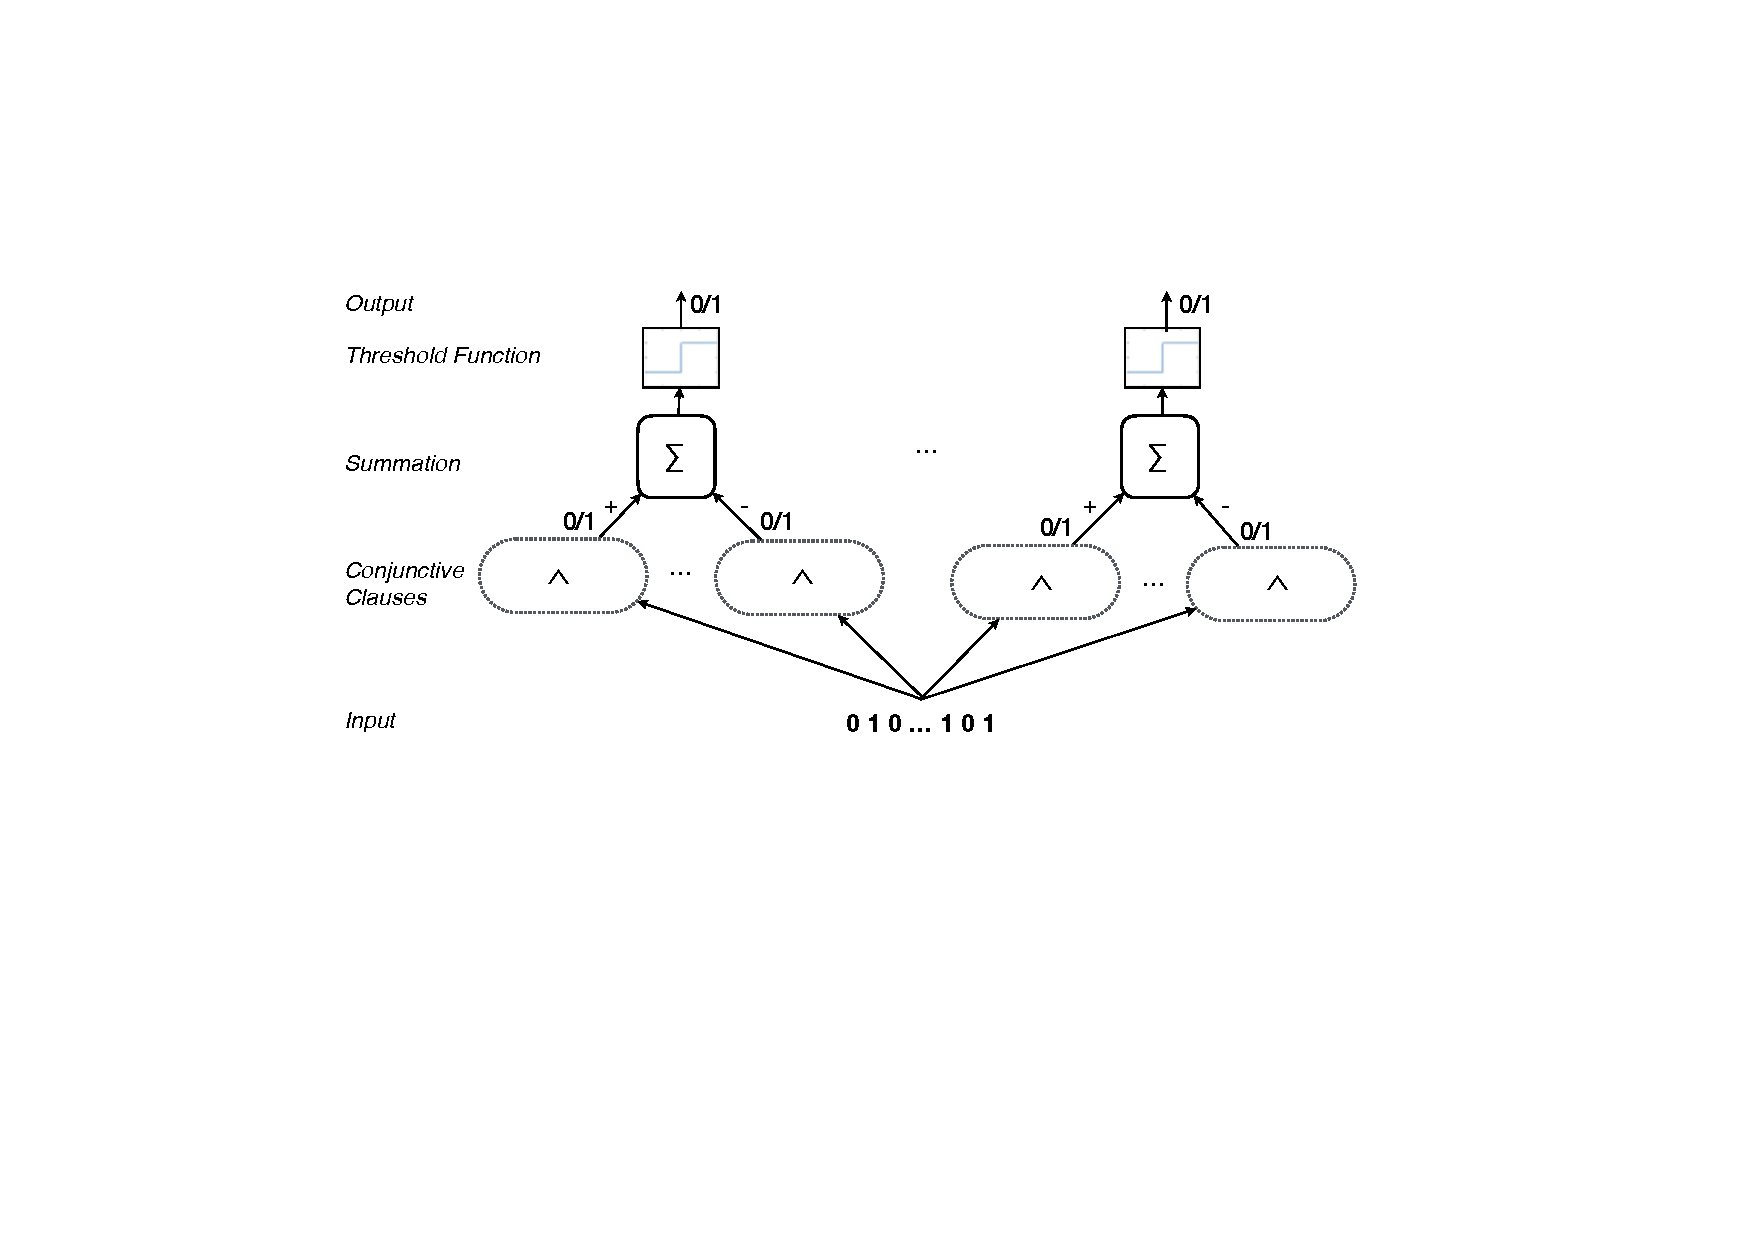
\includegraphics[width=.9\textwidth]{img/Overall_Architecture_Summation[1804.01508v15].pdf}
    \caption[The TM inference structure]{The TM inference structure (source: \cite{granmo2021tsetlinmachinegame})}
    \label{fig:tsetlinmachinestructure}
\end{figure}
\FloatBarrier

\section{Tsetlin Automaton}
The basic building block of a TM is the Tsetlin Automaton (Figure \ref{fig:tsetlinautomatongeneric}), recognized as one of the first solutions to the multi-armed bandit problem~\cite{granmo2021tsetlinmachinegame}. It is capable of learning the optimal action when operating in unknown stochastic environments and is considered the first Learning Automaton~\cite{narendra2012learning}.

\paragraph{Decision making}
The Tsetlin Automaton performs actions $\alpha_z, z \in \{1, 2\}$ sequentially in an environment. Each action $\alpha_z$ triggers a reward or a penalty. The action is rewarded with probability $p_z$, otherwise it is penalized. The reward probabilities are unknown to the automaton and may change over time. Under these conditions, the goal is to identify the action with the highest probability of reward using as few attempts as possible~\cite{granmo2021tsetlinmachinegame}.

\paragraph{State-based memory}
The Tsetlin Automaton operates as a finite-state machine with $2N$ states, as illustrated in Figure \ref{fig:tsetlinautomatongeneric}. The current state determines the action: action $\alpha_1$ is performed in states $1$ to $N$, while action $\alpha_2$ is performed in states $N+1$ to $2N$. State transitions control how the automaton learns. One set of state transitions is activated upon receiving a reward (solid lines in the figure), and another set of state transitions is activated upon receiving a penalty (dotted lines in the figure). This mechanism is designed to reinforce successful (reward producing) actions~\cite{granmo2021tsetlinmachinegame}.

\begin{figure}[!htbp]
    \centering
    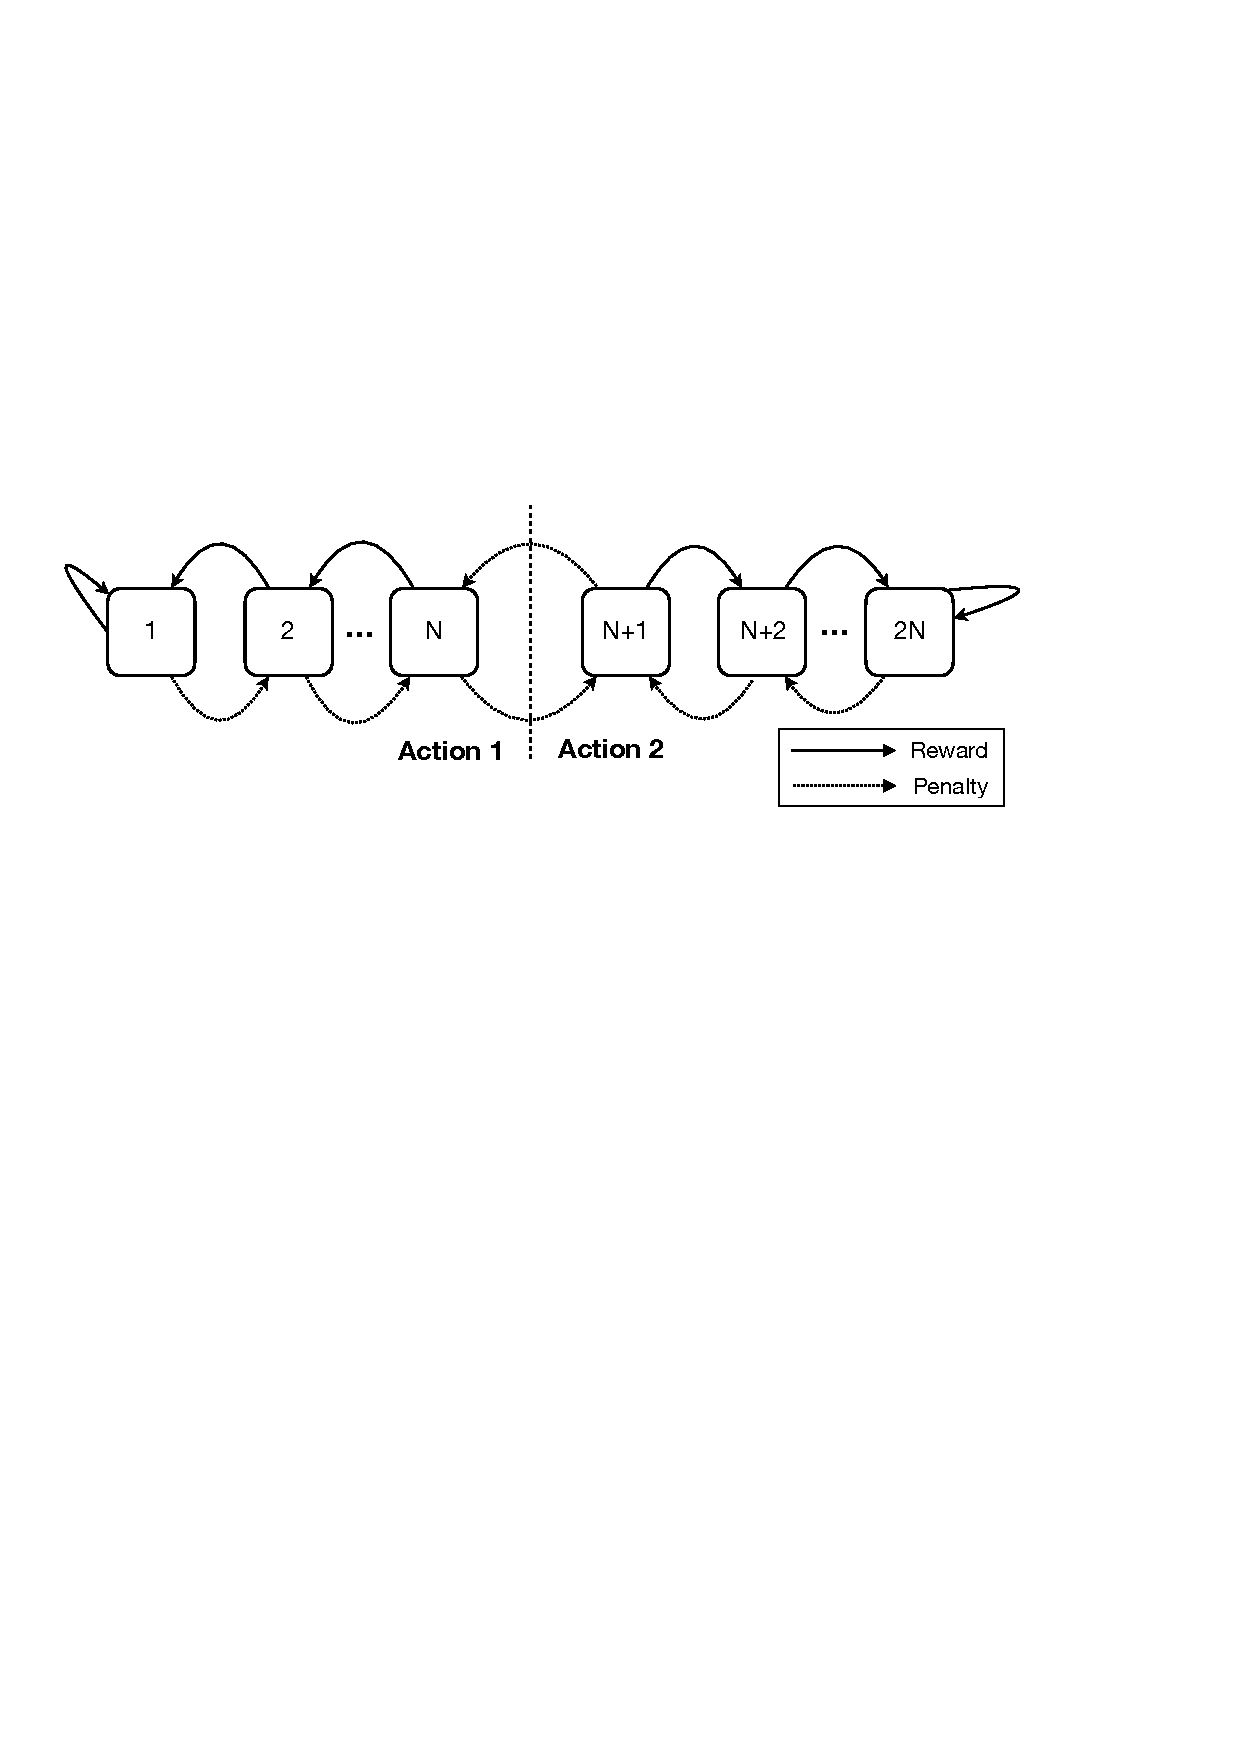
\includegraphics[width=.9\textwidth]{img/Tsetlin_Automaton_Generic[1804.01508v15].pdf}
    \caption[A Tsetlin Automaton for two-action environment]{A Tsetlin Automaton for two-action environment (source: \cite{granmo2021tsetlinmachinegame})}
    \label{fig:tsetlinautomatongeneric}
\end{figure}
\FloatBarrier

\section{Architecture and Problem Representation}
With the Tsetlin Automaton introduced as the main learning mechanism, the TM architecture arranges these automata into teams responsible for composing clauses. These teams collaborate to solve complex problems by optimizing pattern recognition accuracy. The generated clauses function as rules that vote for or against a specific class output while providing transparent logic to reach a final decision~\cite{granmo2021tsetlinmachinegame}. However, this approach requires specific input, where the data must be processed to produce features compatible with logic-based reasoning.

\paragraph{Binarization of data}
Since the TM operates using propositional logic, the input data is required to be represented as Boolean features. Nevertheless, this constraint can be mitigated with a simple pre-processing step that transforms the input into a suitable binary format. For categorical data, the universal one-hot encoding approach will suffice. For example, in the digit recognition problem with $8 \times 8$ images ($64$ elements) and $16$ possible brightness levels, the sample can be flattened and expanded to a binary vector. The handling of continuous features presents a different challenge, commonly addressed by segmenting data into predefined intervals. A continuous variable, such as temperature, can be transformed into a set of Boolean ranges like $[15^\circ,20^\circ)$ or $[20^\circ,25^\circ)$, allowing the machine to simply match the value.

\paragraph{Rule construction}
The mechanism for building a TM involves organizing Tsetlin Automata into teams, where each team is responsible for constructing a single conjunctive clause (AND-rule). These rules follow a logical pattern:
$$\textbf{if} \ \textit{condition} \ \textbf{then} \ \textit{class} \text{.}$$
For every potential literal in the input set (both original features and their negations), an assigned automaton determines whether to ``Include'' or ``Exclude'' that literal based on its internal state~\cite{granmo2021tsetlinmachinegame}. By combining these decisions through the AND-operator, the team produces a logical rule. For the vehicle classification task described in~\cite{granmo2022tsetlinmachinebookchap1}, a resulting rule can be expressed as: 
$$\textbf{if} \ \textit{Four Wheels} \ \textbf{and} \ \textit{Transports People} \ \textbf{then} \ \textit{Car} \text{.}$$

\paragraph{Class prediction by voting}
The TM, as shown in Figure \ref{fig:tsetlinmachinestructure}, feeds an input vector $X = (x_1, \dots, x_n) \in \{0,1\}^n$ to several conjunctive clauses for evaluation. The number of clauses used is a user-defined parameter $N$. The clauses are assigned into two groups based on polarity: positive clauses ($C_j^1, \ j \in \{1,\dots,N/2\}$) vote in favor of the target class ($y=1$), negative clauses ($C_j^0, \ j \in \{1,\dots,N/2\}$) vote against it ($y=0$)~\cite{granmo2021tsetlinmachinegame}.

While a standard clause learns to capture sub-patterns in $X$ and outputs the conjunction of its literals, the TM uses a specific mechanism for empty clauses ($L_j = \emptyset$). These clauses without literals are not required for classification and can be pruned from the inference structure, but during learning, they remain active:
$$C_j(X) = \begin{cases}
1, & \textbf{if } L_j=\emptyset \text{ during learning},\\
0, & \textbf{if } L_j=\emptyset \text{ during classification},\\
\bigwedge_{l_k \in L_j}l_k, & \textbf{if } L_j\neq\emptyset \text{.}
\end{cases}$$
The final classification $\hat{y}$ is reached through a majority vote. The clause evaluations are combined into a final output through summation and unit step thresholding:
$$\hat{y} = u \left( \sum_{j=1}^{N/2}C_j^1(X) - \sum_{j=1}^{N/2}C_j^0(X) \right)$$
where $u(v) = 1 \textbf{ if } v \ge 0 \textbf{ else } 0$. The summation allows the model to weigh positive against negative evidence found in the input $X$. The example classifier that captures the XOR-relation can be represented as $\hat{y} = u(x_1\overline{x}_2 + \overline{x}_1x_2 - x_1x_2 - \overline{x}_1\overline{x}_2)$~\cite{granmo2021tsetlinmachinegame}.

Figure \ref{fig:tsetlinmachineconfiguration} illustrates the TM configuration featuring two clauses: one with positive polarity and one with negative polarity. These clauses are determined by Tsetlin Automata, which select the literals to include from the set $L = \{x_1,x_2,\overline{x}_1,\overline{x}_2\}$. In this example, the positive clause results in the form $x_1\overline{x}_2$, while the negative clause forms $x_1x_2$.

\begin{figure}[!htbp]
    \centering
    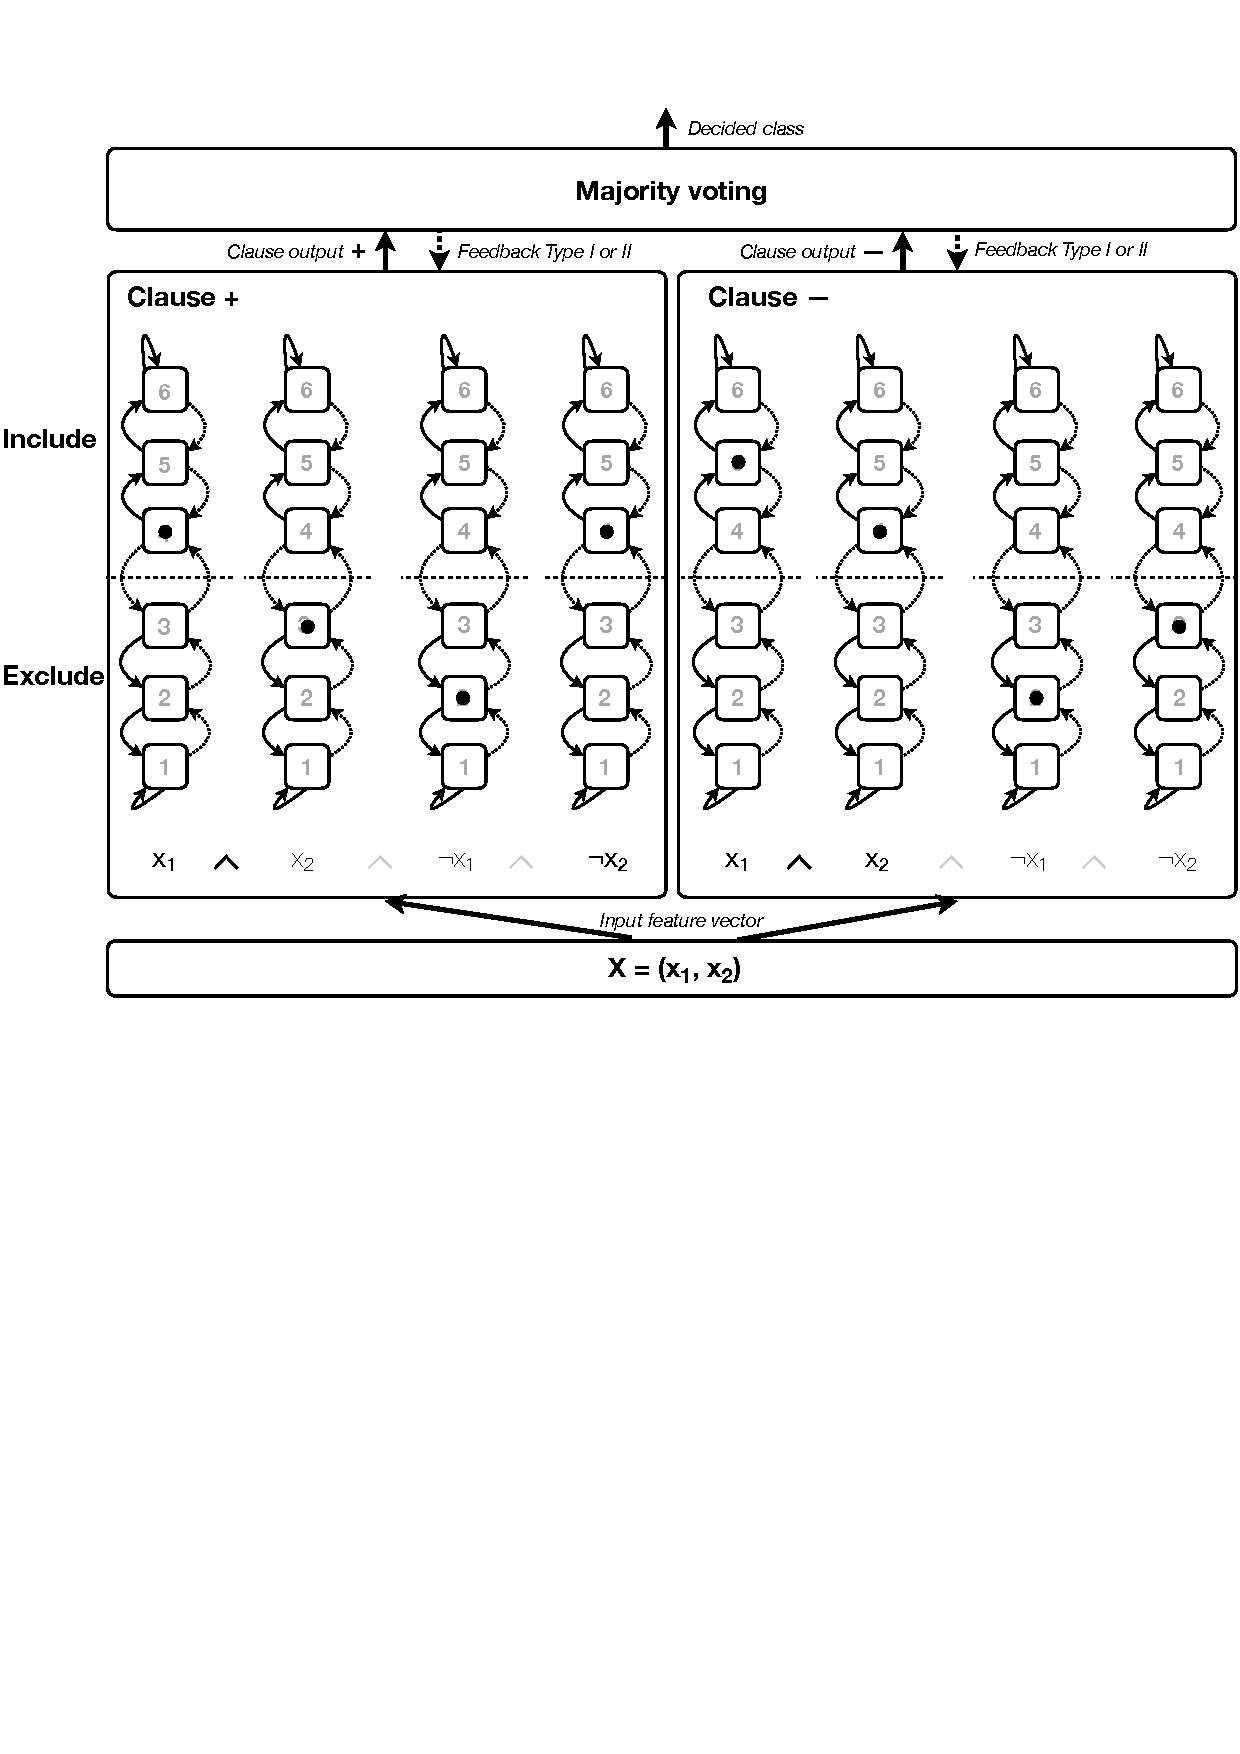
\includegraphics[width=.9\textwidth]{img/Tsetlin_Machine_Example_Configuration_Full[1804.01508v15].pdf}
    \caption[Two Tsetlin Automata teams]{Two Tsetlin Automata teams, each producing a conjunctive clause (source: \cite{granmo2021tsetlinmachinegame})}
    \label{fig:tsetlinmachineconfiguration}
\end{figure}
\FloatBarrier

\section{Learning Algorithm}
The learning mechanism of the TM functions through a game-theoretic approach, orchestrating Tsetlin Automata to maximize pattern recognition accuracy~\cite{granmo2021tsetlinmachinegame}. We follow the example found in~\cite{glimsdal2021coalescedmultioutputtsetlinmachines} to demonstrate this process.

\paragraph{IMDb review sentiment example}
To demonstrate the learning process, we consider the task of classifying the sentiment of movie reviews from the IMDb dataset. This problem uses a Set of Words (SoW) representation, where every word in the vocabulary acts as an input feature. Consider the review ``The movie was good, and I had popcorn.''. This text is converted into a binary input vector $X$. The inputs for words present in the review (e.g. ``good'' and ``movie'') are set to True, while the inputs for any missing words are set to False.

\paragraph{Memory}
Consider the clause designed to detect positive sentiment targeting the pattern ``good'' AND ``movie''. To manage this rule, the machine uses a team of Tsetlin Automata, assigning one automaton to track each potential literal. Figure \ref{fig:memoryimdb} illustrates the memory states maintained by this team. Feedback from the learning process increases these states to remember the literal longer when a reinforcing truth value is observed, and without such observations, the values decrease, causing the clause to eventually forget the literal.

\begin{figure}[!htbp]
    \centering
    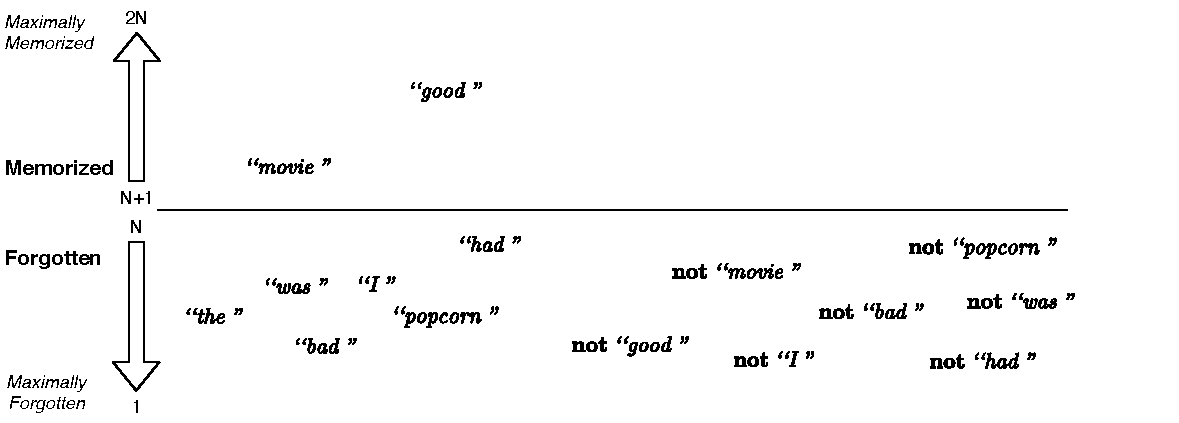
\includegraphics[width=.9\textwidth]{img/Memory_IMDb[2108.07594v1].pdf}
    \caption[Sticky memory for IMDb example]{Sticky memory for IMDb example with depth N for the clause: ``good'' AND ``movie'' (source: \cite{glimsdal2021coalescedmultioutputtsetlinmachines})}
    \label{fig:memoryimdb}
\end{figure}
\FloatBarrier

\paragraph{Memory updating}
Memory is updated on a specific input $X$ to the TM. A user-defined parameter $s$ controls how quickly truth values are forgotten. In result, increasing $s$ makes the patterns finer (more specific), while decreasing $s$ makes them coarser (more general). The process of updating the memory of each clause is handled by these three operators~\cite{glimsdal2021coalescedmultioutputtsetlinmachines}:
\begin{compactitem}
    \item The $\textbf{memorize}(X,s)$ operator handles \textbf{Type Ia feedback} (Figure \ref{fig:memoryimdbtypeIa}). It strengthens the memory of an input $X$ by increasing integer values for truth values present in $X$. Simultaneously, truth values that conflict with the input have their integers decreased randomly with probability $\frac{1}{s}$.
    \item The $\textbf{forget}(s)$ operator handles \textbf{Type Ib feedback} (Figure \ref{fig:memoryimdbtypeIb}). It performs forgetting by randomly decreasing the memory integer of all truth values with probability $\frac{1}{s}$. This gradually moves all literals towards the ``maximally forgotten'' state.
    \item The $\textbf{invalidate}(X)$ operator handles \textbf{Type II feedback} (Figure \ref{fig:memoryimdbtypeII}). It adjusts the clause to reject the input $X$ by increasing the memory integer of all False truth values. For instance, if the word ``bad'' appears in a negative review that was incorrectly classified, the system increases the integer for \textbf{not} ``bad''.
\end{compactitem}

\begin{figure}[!htbp]
    \centering
    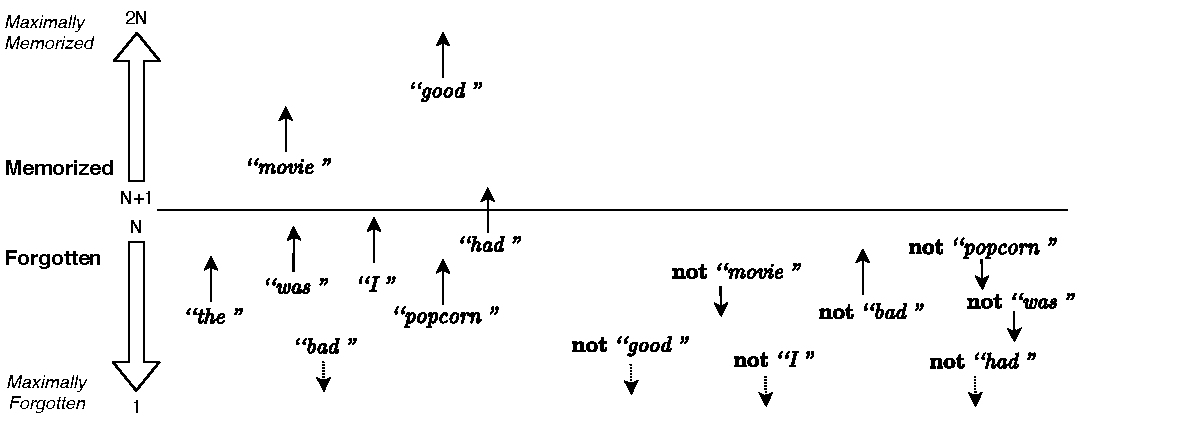
\includegraphics[width=.9\textwidth]{img/Memory_IMDb_Type_Ia[2108.07594v1].pdf}
    \caption[Type Ia feedback for IMDb example]{Type Ia feedback triggered by input ``The movie was good, and I had popcorn.'' (source: \cite{glimsdal2021coalescedmultioutputtsetlinmachines})}
    \label{fig:memoryimdbtypeIa}
\end{figure}
\FloatBarrier

\begin{figure}[!htbp]
    \centering
    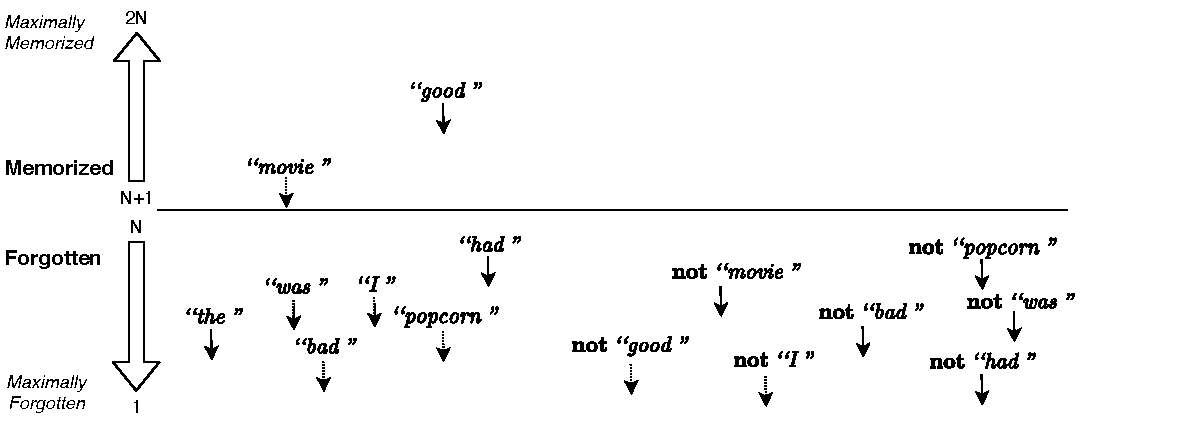
\includegraphics[width=.9\textwidth]{img/Memory_IMDb_Type_Ib[2108.07594v1].pdf}
    \caption[Type Ib feedback for IMDb example]{Type Ib feedback triggered by input ``Was good, and I had popcorn.'' (source: \cite{glimsdal2021coalescedmultioutputtsetlinmachines})}
    \label{fig:memoryimdbtypeIb}
\end{figure}
\FloatBarrier

\begin{figure}[!htbp]
    \centering
    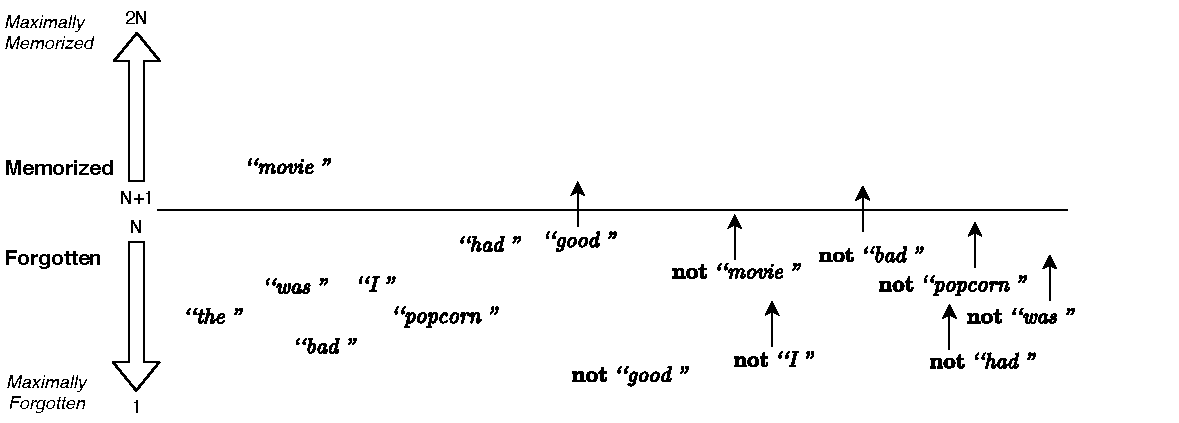
\includegraphics[width=.9\textwidth]{img/Memory_IMDb_Type_II[2108.07594v1].pdf}
    \caption[Type II feedback for IMDb example]{Type II feedback applied to input ``The movie was bad, and I had popcorn.'' (source: \cite{glimsdal2021coalescedmultioutputtsetlinmachines})}
    \label{fig:memoryimdbtypeII}
\end{figure}
\FloatBarrier

\paragraph{Learning single clauses}
Prediction outcomes guide the learning of each TM clause~\cite{glimsdal2021coalescedmultioutputtsetlinmachines}:
\begin{compactitem}
    \item \textbf{True Positive}: The clause correctly votes for its assigned output. In this case, the clause performs $\textbf{memorize}(X,s)$. This feedback makes the clause remember and refine the pattern it recognizes in $X$.
    \item \textbf{False Negative}: The clause fails to vote for its assigned output. In this case, the clause performs $\textbf{forget}(s)$. This reinforcement coarsens infrequent patterns, making them frequent.
    \item \textbf{False Positive}: The clause incorrectly votes for its assigned output. The clause then performs $\textbf{invalidate}(X)$. This feedback makes the clause more discriminative.
    \item \textbf{True Negative}: The clause correctly refrains from voting for its assigned output. This outcome does not trigger any memory updates.
\end{compactitem}

\paragraph{Learning multiple clauses}
The TM achieves coordination by introducing another parameter, a voting margin $t$. This ensures that a sufficient number of clauses support each output without using more clauses than necessary. Learning multiple clauses works as follows~\cite{glimsdal2021coalescedmultioutputtsetlinmachines}:
\begin{compactenum}
    \item \textbf{Input:} Consider a training sample of truth values $X$ and the target truth value $y$.
    \item \textbf{Vote Aggregation:} Compute the net voting sum $v$ by aggregating the output of all clauses that evaluate to \textit{True} on input $X$. Votes in favor of the target class $y$ are positive, while votes in favor of $\textbf{not } y$ are negative. The final sum $v$ is clipped to the range $[-t, t]$.
    \item \textbf{Stochastic Update:} A feedback update for each clause is triggered with probability $P_\text{update} = \frac{t-v}{2t}$. If triggered, the clause is modified as follows:
    \begin{compactenum}
        \item \textbf{True Positives (Type Ia feedback):} Perform $\textbf{memorize}(X,s)$ (the clause matches $X$ and outputs $y$)
        \item \textbf{False Negatives (Type Ib feedback):} Perform $\textbf{forget}(s)$ (the clause does not match $X$ and outputs $y$)
        \item \textbf{False Positive (Type II feedback):} Perform $\textbf{invalidate}(X)$ (the clause matches $X$ and outputs $\textbf{not } y$)
    \end{compactenum}
\end{compactenum}

\paragraph{XOR-gate example}
Figure \ref{fig:tsetlinmachinexorgate} illustrates the learning process for an XOR-gate training sample with input $(x_1=0,x_2=1)$ and target output $y=1$. Initially (Step $1$), the positive clauses $C_1$ and $C_3$ do not match the input because they contain conflicting literals (e.g. $\overline{x_2}$ in $C_3$ conflicts with $x_2=1$). This results in a false negative prediction,. which triggers Type Ib feedback. This feedback forces the clause to forget the conflicting literals. Once the clauses are generalized enough to match the input, Type Ia feedback reinforces inclusion of valid literals present in the input (e.g. $x_2$ in $C_3$). By Step $t$, these updates modified Clause $C_1$ to $\overline{x_1}x_2$ and $C_3$ to just $x_2$ allowing the machine to match the input and produce the correct prediction $\hat{y}=1$.

\begin{figure}[!htbp]
    \centering
    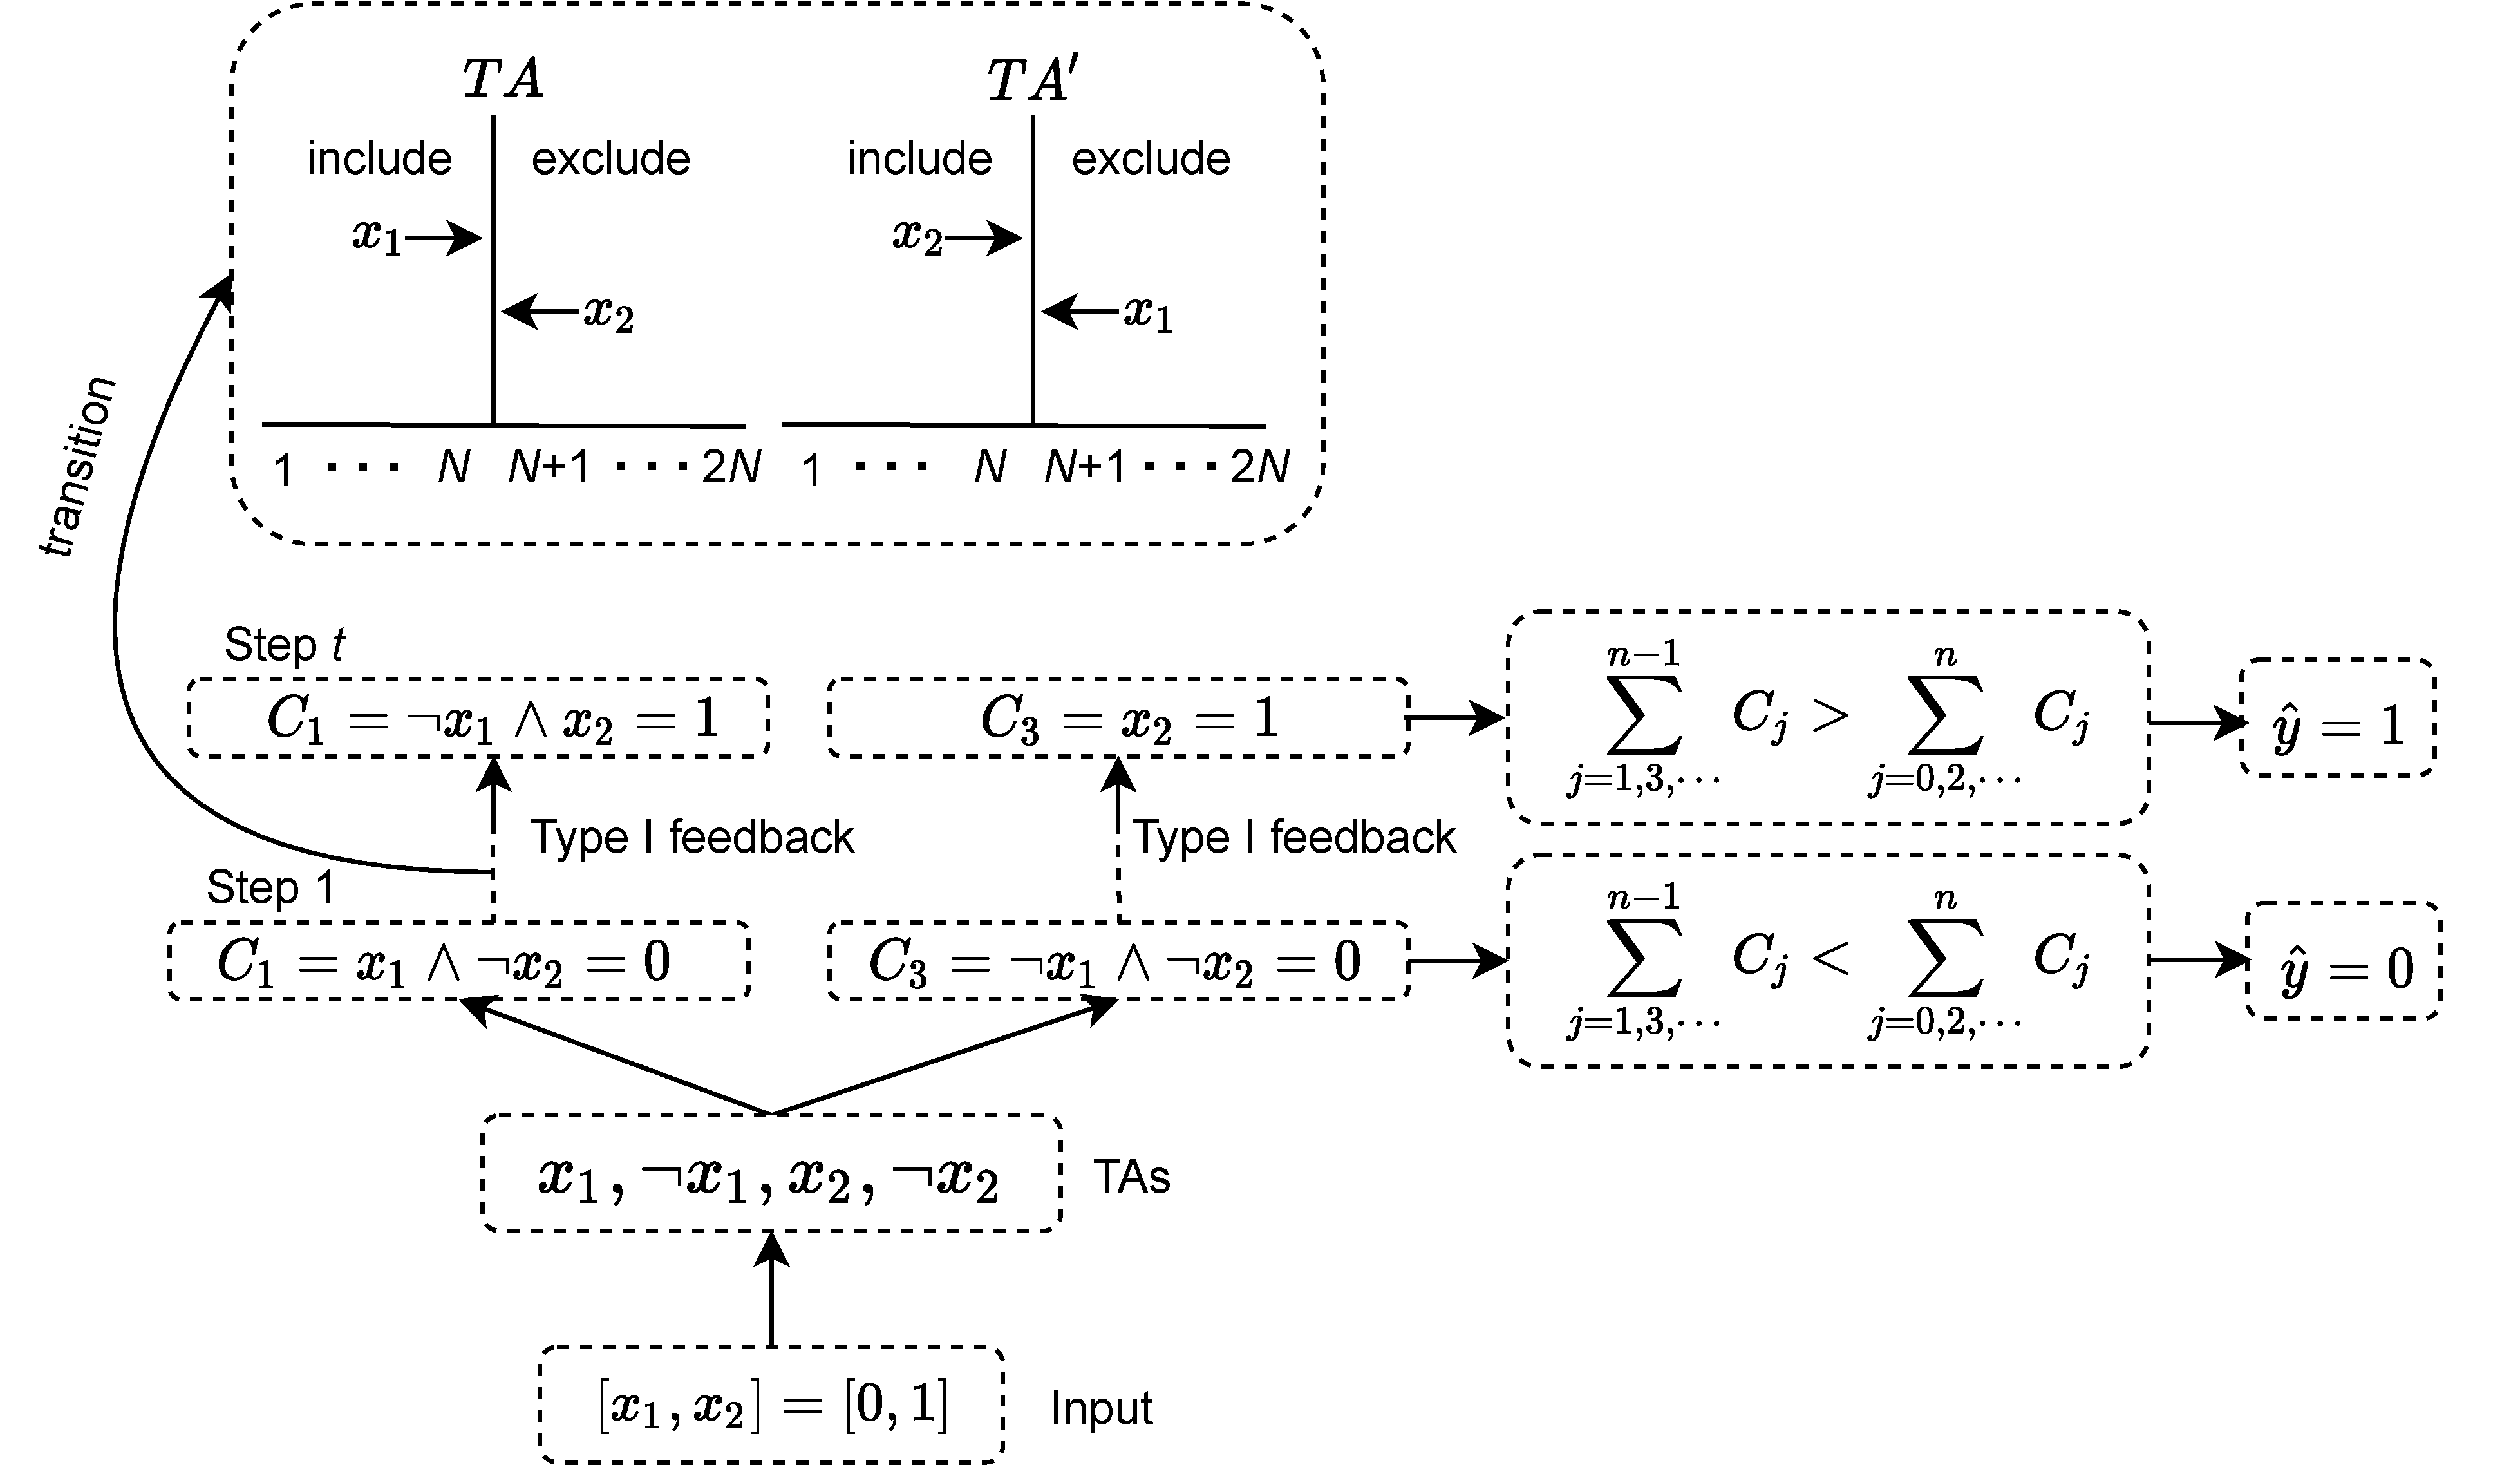
\includegraphics[width=.9\textwidth]{img/TM[arXiv-2212.13634v1].pdf}
    \caption[TM XOR-gate training]{TM learning dynamics for an XOR-gate training sample, with input $(x_1 = 0, x_2 = 1)$ and output target $y = 1$ (source: \cite{sharma2022equivalenceweightedtsetlinmachine})}
    \label{fig:tsetlinmachinexorgate}
\end{figure}
\FloatBarrier

\section{Tsetlin Machine Architecture Variants}
Due to the modular design of the original TM, there is an ongoing effort to further develop this method. Researchers have implemented new iterations to address and mitigate limitations discovered in the original design. In this section, we briefly discuss three significant architectural variations and what they attempt to accomplish.

\paragraph{The Coalesced Tsetlin Machine}\label{para:cotm}
The standard design of the TM supports prediction for only a single binary output. Multi-output problems require a workaround where a separate machine is created for every output. This approach in which each machine works independently limits the ability to share patterns that may be relevant to multiple classes. The Coalesced TM~\cite{glimsdal2021coalescedmultioutputtsetlinmachines} introduces a shared pool of clauses. This is accomplished by a weight matrix that connects every clause to every possible output. Instead of a rule belonging to just one class, it is assigned an integer weight: a positive weight votes in favor of a class, while a negative weight votes against it. Empirical results on benchmark datasets show that this approach obtains significantly higher accuracy in 50 to 1000-clause configurations, indicating an ability to reuse clauses and stronger robustness against imbalanced training data~\cite{glimsdal2021coalescedmultioutputtsetlinmachines}. Figure \ref{fig:tsetlinmachinecoalesced} shows an inference structure with three outputs, a newly introduced clause memory matrix and a clause weight matrix.

\begin{figure}[!htbp]
    \centering
    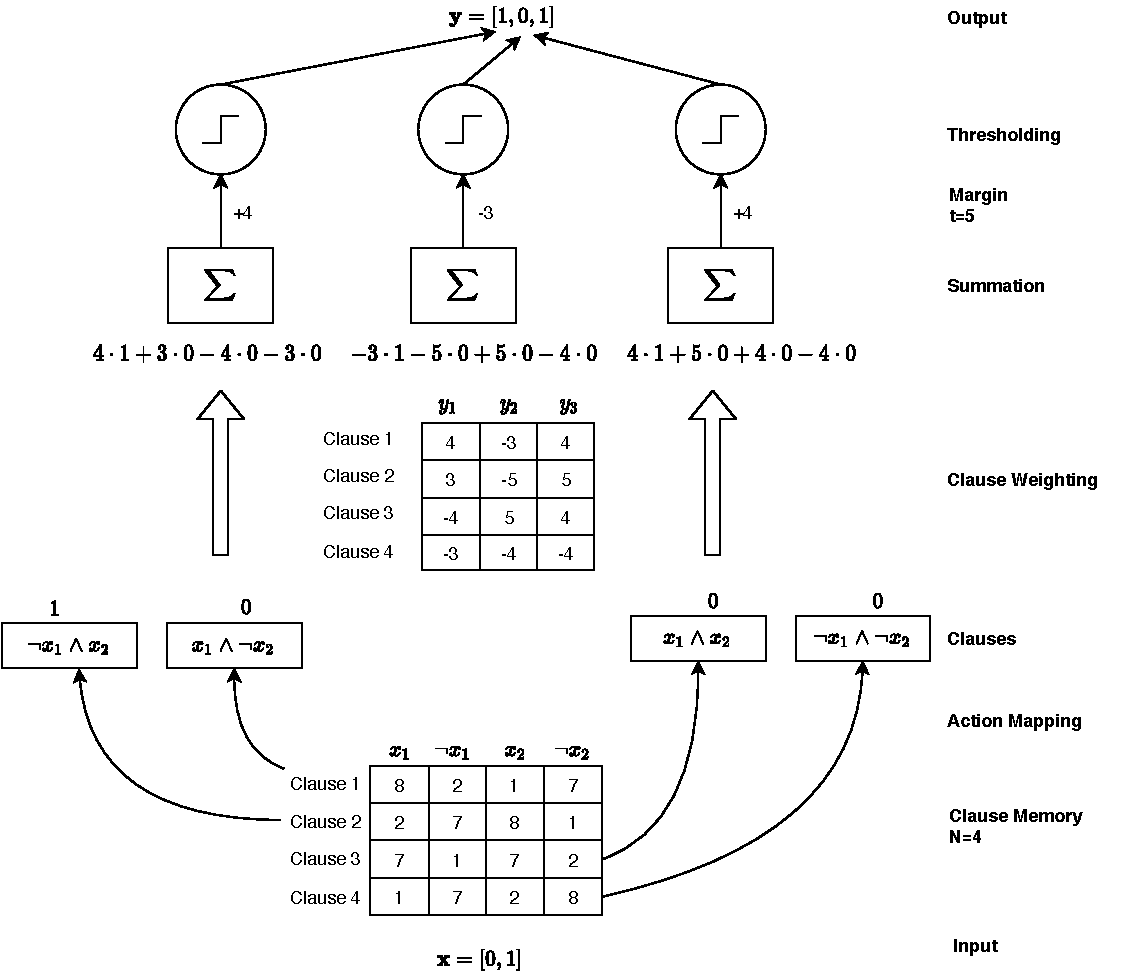
\includegraphics[width=.9\textwidth]{img/CoalescedMultiOutputTM[2108.07594v1].pdf}
    \caption[The Coalesced TM structure]{The Coalesced TM structure with inference example (source: \cite{glimsdal2021coalescedmultioutputtsetlinmachines})}
    \label{fig:tsetlinmachinecoalesced}
\end{figure}
\FloatBarrier

\paragraph{The Sparse Tsetlin Machine}
The standard TM maintains the entire state space, storing a significant number of unnecessary values that consume memory and computational time. The Sparse TM~\cite{glimsdal2024sparsetsetlinmachine} addresses this by implementing the \textit{Active Literals} mechanism, which focuses resources only on actively contributing literals. To achieve this, the architecture utilizes the Compressed Sparse Row (CSR) format and discards negated features, assuming that any missing feature is implicitly negated. A lower-bound threshold is added to ensure the compactness of the model, where any literal state reduced below the limit is removed from the clause. This significantly reduces memory footprint and computational time while maintaining competitive classification performance~\cite{glimsdal2024sparsetsetlinmachine}. Figure \ref{fig:tsetlinmachinesparse} illustrates the feedback interaction between \textit{Active Literals} and sparse clauses. During Type Ia feedback (reinforcing true positives), \textit{Active Literals} identify and store meaningful literals, while Type II feedback (combating false positives) introduces these literals into the sparse clauses to invalidate incorrect matches.

\begin{figure}[!htbp]
    \centering
    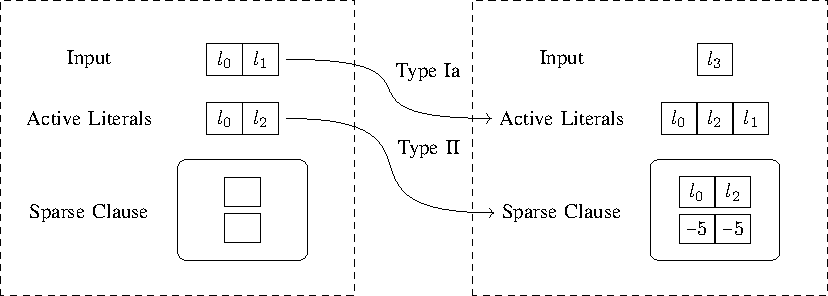
\includegraphics[width=.9\textwidth]{img/sparse_al_populate[arXiv-2405.02375v2].pdf}
    \caption[The Sparse TM Active Literals]{The Sparse TM using Active Literals (source: \cite{glimsdal2024sparsetsetlinmachine})}
    \label{fig:tsetlinmachinesparse}
\end{figure}
\FloatBarrier

\paragraph{The Stateless (Inference Only) Tsetlin Machine}
There is a major difference between how the TM learns and how it makes predictions. During the learning phase, the machine relies on a detailed memory state to track pattern confidence, storing a state integer (ranging from $1$ to $2N$) for every potential literal. However, once training is completed, this detailed history is no longer needed to make predictions. For inference, the model only needs to know which specific literals to Include and which to Exclude, converting complex memory states into simple binary rules. By discarding learning memory and keeping only the final compiled rules, the model significantly reduces memory usage during deployment when on-device learning is not required. For example, in Figure \ref{fig:memoryimdb}, the inference model would discard the forgotten values and store only the final rule: ``good'' AND ``movie''.

\section{Comparison with Neural Networks}
Neural Networks are currently the standard approach for AI applications, making them the common benchmark for new methods. For a direct theoretical comparison, the research conducted in~\cite{sharma2022equivalenceweightedtsetlinmachine} introduced the Weighted TM. This architecture assigns an integer weight to each clause based on its prediction accuracy, operating similarly to the Coalesced TM (Section \ref{para:cotm}) but without the clause sharing mechanism. With this modification, the TM behaves as a special case of a perceptron using logical clauses as binary inputs instead of raw features~\cite{sharma2022equivalenceweightedtsetlinmachine}.

The difference in the decision boundaries on the Iris dataset is illustrated in Figure \ref{fig:decisionboundaryvis}, where each model was trained for $50$ epochs. The TM (Figure \ref{fig:tsetlinmachinevis}) used 50 clauses and the Single Layer Neural Network (Figure \ref{fig:neuralnetworkvis}) utilized 50 neurons. The TM builds its decision boundaries from the binary output of individual clauses ($C_i = \{0, 1\}$). It results in steps formed by filling contour lines rather than the smooth curves generated by neural networks. This difference changes how each model adapts to new data. In the TM, a clause (or a set of clauses) can simply learn the new pattern and create a step in the decision boundary to include the new data point in the correct region~\cite{sharma2022equivalenceweightedtsetlinmachine}.

\begin{figure}[!htbp]
    \centering
    % Subfigure 1
    \begin{subfigure}{0.3\textwidth}
        \centering
        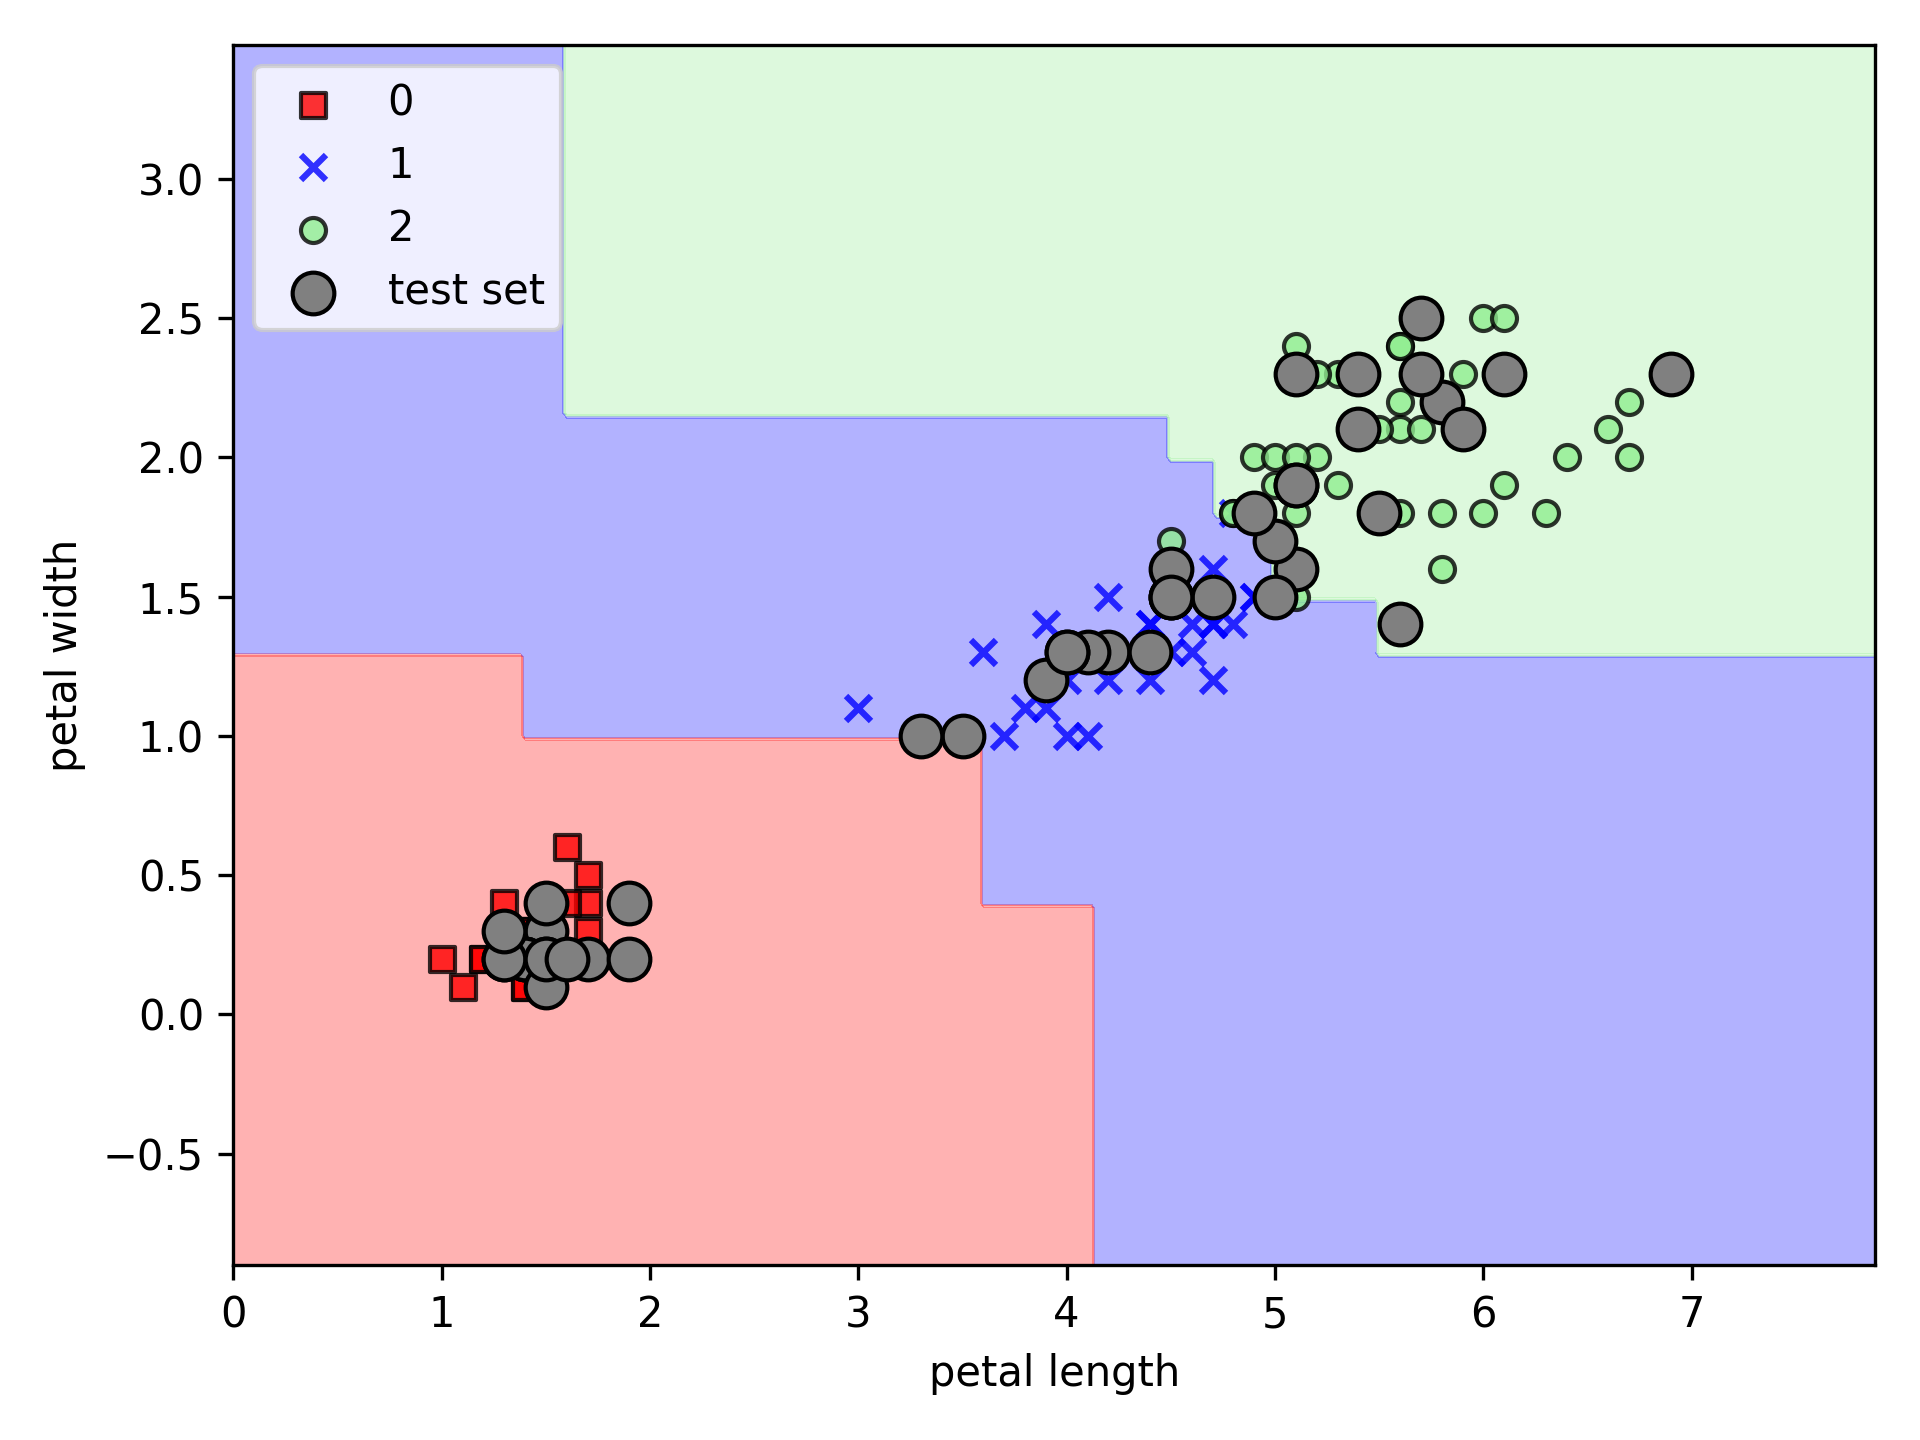
\includegraphics[width=\textwidth]{img/tm_vis[arXiv-2212.13634v1].png}
        \caption{TM}
        \label{fig:tsetlinmachinevis}
    \end{subfigure}
    \hfill
    % Subfigure 2
    \begin{subfigure}{0.3\textwidth}
        \centering
        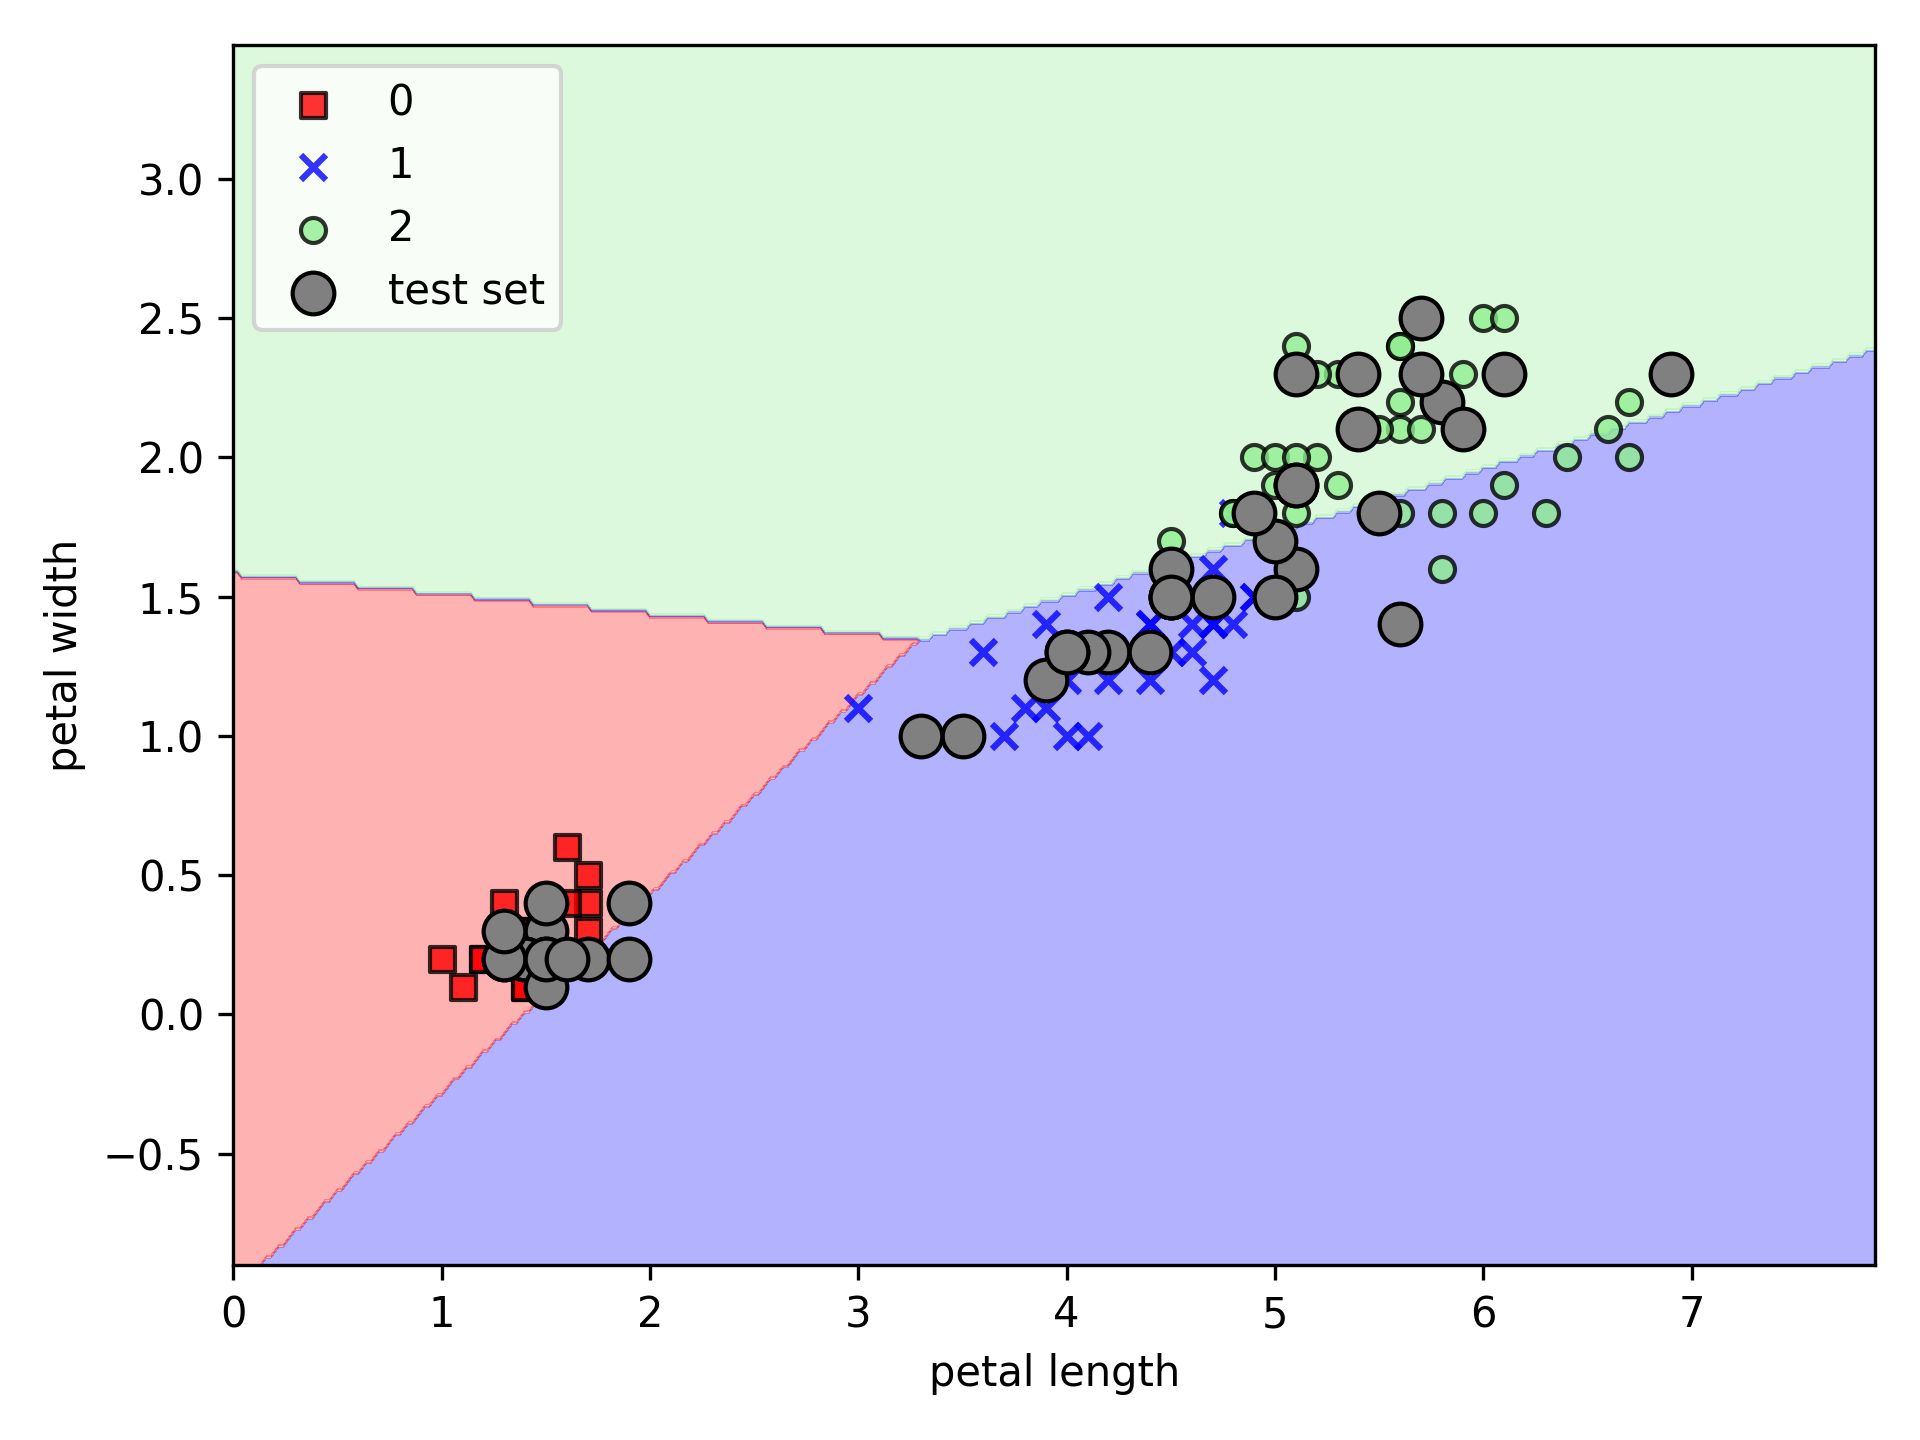
\includegraphics[width=\textwidth]{img/perceptron_vis[arXiv-2212.13634v1].png}
        \caption{Perceptron}
        \label{fig:perceptronvis}
    \end{subfigure}
    \hfill
    % Subfigure 3
    \begin{subfigure}{0.3\textwidth}
        \centering
        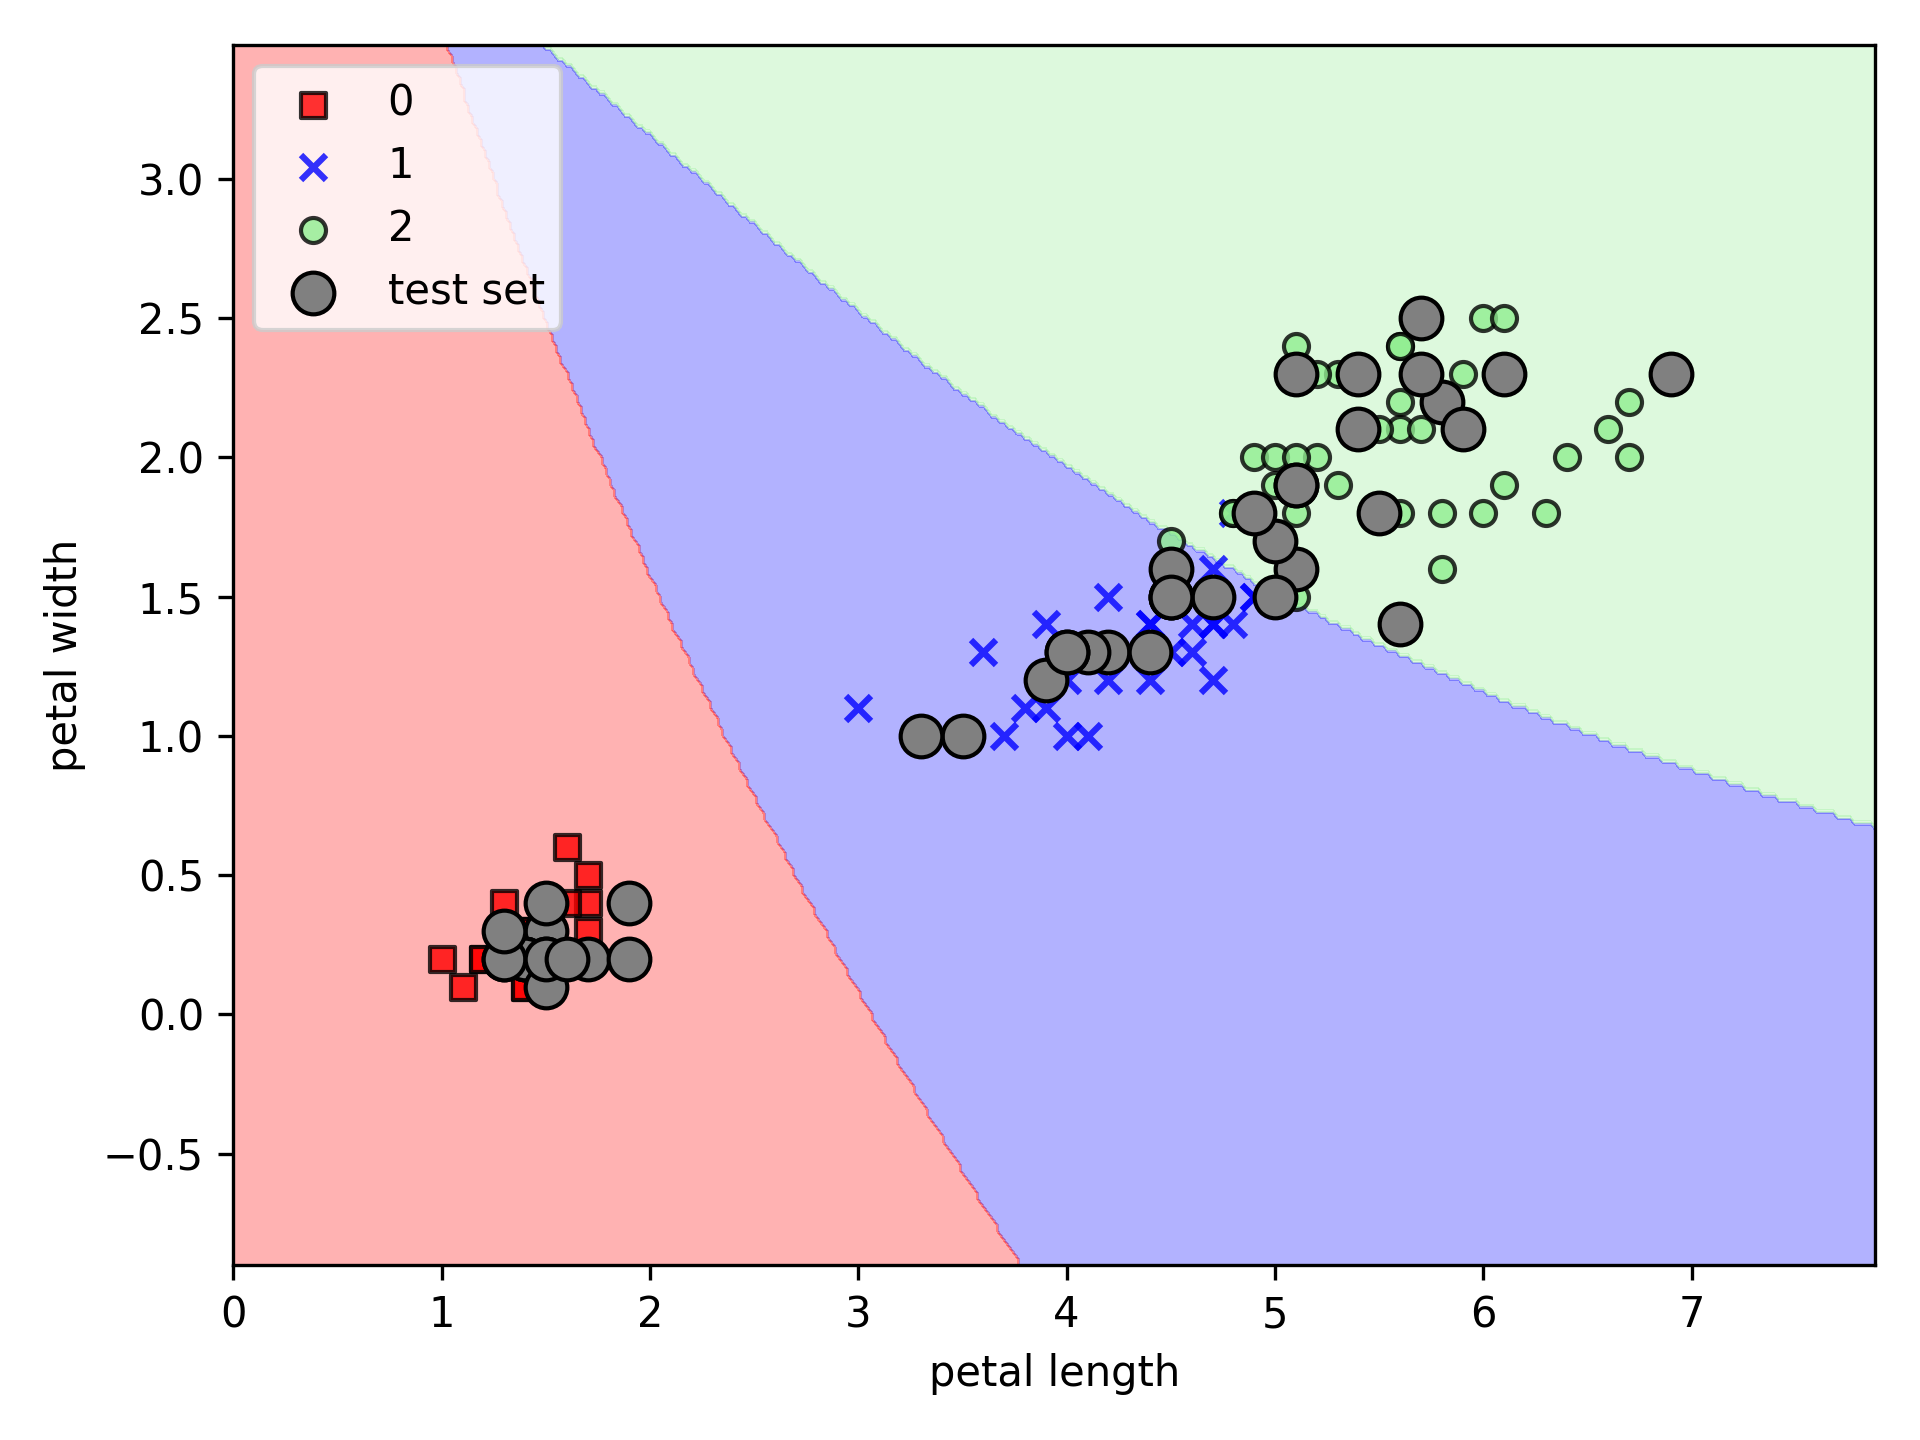
\includegraphics[width=\textwidth]{img/mlp_vis[arXiv-2212.13634v1].png}
        \caption{Single Layer NN}
        \label{fig:neuralnetworkvis}
    \end{subfigure}

    \caption[Decision boundary visualization]{Decision boundary visualization on the Iris dataset (source: \cite{sharma2022equivalenceweightedtsetlinmachine})}
    \label{fig:decisionboundaryvis}
\end{figure}
\FloatBarrier

\paragraph{Transparent logic}
Neural networks are often described as ``black boxes'' because their decision making logic is hidden and difficult for humans to interpret. This contrasts with the TM, where interpretability comes naturally from its logic-based approach. The produced rules are human-readable clauses (e.g. \textit{if X and Y then Class A}), making it technically possible to even manually add or edit rules. This transparency allows users to examine the inner workings in applications where understanding the reasoning behind a prediction is mandatory.

\paragraph{Computational efficiency and optimization}
An important difference between the architectures lies in their underlying arithmetic. Neural networks typically rely on floating-point matrix multiplications that require substantial computational resources. In contrast, the TM operates primarily using bitwise operators (AND, OR, NOT) and simple integer arithmetic. Theoretically, this offers efficiency advantages, enabling implementations on hardware lacking dedicated floating-point units. However, modern processors such as GPUs and TPUs are specifically engineered to accelerate matrix operations, since they are widespread in fields ranging from physics simulations to deep learning. As a result, the performance advantage of an integer-based approach is diminished on hardware that implements these optimizations.

\paragraph{Performance with limited data}
According to research presented in~\cite{granmo2021tsetlinmachinegame}, TMs generalize better with smaller datasets compared to neural networks. In benchmarks such as the Noisy XOR problem, the TM maintained much higher accuracy on smaller datasets, whereas neural networks required larger datasets to converge. This makes the TM a suitable candidate for environments where data is limited or noisy.

\section{Summary}
In conclusion, the Tsetlin Machine is a logic-based alternative for pattern recognition that utilizes Boolean algebra. It is built upon Tsetlin Automata, which are finite-state machines that learn optimal actions through rewards and penalties. These automata are arranged into teams to construct ``If-Then'' rules known as conjunctive clauses, which identify sub-patterns in data. Then these clauses are for or against a target class to reach a final decision. The model is trained using a game-theoretic algorithm that employs different types of feedback to memorize, forget, or invalidate patterns. Compared to traditional ``black box'' neural networks, the Tsetlin Machine benefits from transparent logic and efficiency, both with computational resources and training data. Finally, recent architectural variants such as Coalesced, Sparse, and Stateless Tsetlin Machines address limitations of the original design.
\chapter{Functional Scope}
\label{chap:functional-scope}

This chapter outlines the considerations and requirements for the library and the supporting tools. Describes the intended audience and details the key decisions made during development. These choices are further described in subsequent sections on Functional and Non-functional requirements.

\section{Expected User Groups}
Due to the experimental nature of this work, the key design goal was to make the library both easy to use and easy to understand. This is necessary as we anticipate that users may need to adapt the library for integration into their specific applications.

\paragraph{Embedded developers}
The library was designed with the limitations of embedded hardware in mind. Unlike many alternatives, it supports every step of the process on-device, while others implement predictions on-device only. Thanks to the designed model exchange format, users can choose to train models on faster hardware or use the \GreenTsetlinName library to later move them to the edge device. Additionally, the efficiency gains promised by TMs~\cite{granmo2021tsetlinmachinegame} are highly beneficial for these resource limited devices, where standard machine learning methods are often too expensive or complicated to run.

\paragraph{Researchers}
As TMs have only recently started to gain recognition, we expect researchers familiar with classic machine learning models to benefit from integrating them into their workflows. By offering a familiar interface, our library enables rapid prototyping. This distinguishes our solution from others that require deeper domain knowledge, making it easier to benchmark the models in various use cases.

\section{Functional Requirements}

\paragraph{On-device training and inference}
Our solution was designed to support both TM training and inference directly on target hardware. Unlike other embedded machine learning frameworks that perform only inference on edge devices, this library enables the model to learn directly from newly gathered data. This is necessary for applications that adapt to local sensor data without a constant connection to the central server.
It should however facilitate an inference only mode with a lighter model serialization format specifically for more resource constrained systems.

\paragraph{Interoperability and serialization}
The library must implement functionality for saving and loading model states. This requires a standardized serialization format to ensure compatibility with the \GreenTsetlinName library. This compatibility is essential for the users to leverage high-performance workstations to pre-train models, export them, and then deploy them directly to the embedded devices. Furthermore, models trained or tuned on the edge must also be exportable for backup or analysis on faster hardware.

\paragraph{Configurable hyperparameters}
Exposing TM model hyperparameters is necessary for fitting the model to its application with varied limitations dictated by hardware or the input data itself. Researchers and developers must be able to easily fine-tune these parameters when designing their solution for each specific problem. This allows optimization of performance, memory footprint, or accuracy without modifying library code. 

\paragraph{Correctness with the theoretical work}
The implementation must behave as described in theoretical research~\cite{granmo2021tsetlinmachinegame}. It is required to accurately model the Tsetlin Automata logic and implement the specific learning rules (Type I and Type II feedback) defined in the original papers. This ensures that the software is a close representation of the method proposed in the theory and avoids unintended assumptions.

\section{Nonfunctional Requirements}

\paragraph{Portability}
The library must be designed for compatibility, avoiding dependencies on any specific hardware or operating system. The functionality of the external library should be defined during compilation if there is a risk that it may not work on the desired target. This strategy ensures that the code can be compiled with minimal, if any, modifications for a wide range of hardware architectures. The resulting portability, coupled with the adjustable model parameters, allows end users to create a solution that is both widely adoptable and future-proof.

\paragraph{Performance and memory usage}
Optimizations are significantly beneficial, as the library's performance impacts both the training step and, more importantly, the real-time predictions on target devices. Given that TMs heavily rely on binary logic and random number generators, optimizing these areas allows for better utilization of limited hardware resources. This optimization extends to memory management, since the memory is needed to store the model on the device, as well as the memory used during runtime, must also be considered.

\paragraph{Simple API}
The Applications Programming Interface (API) must be intuitive and well-documented. Its design should follow standard interfaces developed by major machine learning libraries, allowing users unfamiliar with TM theory to quickly prototype concepts. This simple interface allows a developer to easily integrate the library into an existing project. Moreover, supporting quick prototyping in environments like Python Jupyter Notebooks alongside established models from libraries such as Scikit-learn speeds up development before deployment to embedded devices.

\paragraph{Testing and examples}
As with any software project, testing enhances the development process and maintenance. Code examples provide a starting point for users unfamiliar with the project. Furthermore, simple installation and easy to run examples encourage potential users to quickly try the library. Finally, these tests help verify that the library runs correctly on new devices with different hardware limitations.
\chapter{Selected Realization Aspects}
\label{chap:realization-aspects}

This section describes the design choices of \LibraryName as well as the rationale behind them, and the overarching architecture of the solution. The actual TM implementation is described in detail to make it intuitive. It describes used tools, solutions and algorithms. Additionally, it discusses several interesting problems that were encountered.

\section{System Architecture and Data Workflow}\label{sec:system-architecture}
The project's architecture and data flow are shown in Figure \ref{fig:projectdiagram}. The design is split between a \textbf{host (PC)} and an \textbf{embedded device}, allowing models to be developed on one platform and transferred to different hardware for deployment.

\paragraph{Training and exporting}
The process starts by defining and training TM models using an external library (\textbf{C}). In this project, we use the \GreenTsetlinName library. Once training is complete, our Python Interface (\textbf{G}) handles exporting the model. We support two different interchange formats:
\begin{compactitem}
    \item FlatBuffers~\cite{flatbuffers} (\textbf{D}) - An efficient, cross-platform serialization format utilizing a third-party library.
    \item Custom Binary (\textbf{E}) - A dependency-free format that may require adjustments based on the target hardware.
\end{compactitem}

\paragraph{On-device execution}
After the serialized model state (\textbf{I}) is saved, it can be moved to the embedded device. On the device, we use our core library (\textbf{O}), which supports every step of the machine learning workflow:
\begin{compactitem}
    \item It can load a pretrained model (\textbf{K}) to start making predictions (\textbf{N}) immediately.
    \item It can be trained further on the device (\textbf{L}) using data gathered during operation (\textbf{P}).
    \item It can save and export the updated model state (\textbf{M}) to back up or inspect what the device has learned.
    \item It also supports creating new models (\textbf{J}) directly on the device if needed.
\end{compactitem}

\paragraph{Python integration}
Since the core library is self-sufficient, it can also be compiled for the host architecture. This allows us to provide a Python package with bindings to the same C code, so that it can run on a standard computer. This package includes a \textit{Scikit-learn}-like interface (\textbf{F}) and is easy to install, similar to other common machine learning tools. This enables rapid testing of ideas in \textit{Jupyter Notebooks} (\textbf{H}) and makes it possible to benchmark our implementation against standard models provided by Python libraries.

\begin{figure}[!htbp]
\centering
\begin{tikzpicture}[scale=0.7, transform shape]
\pgfdeclarelayer{background}
\pgfsetlayers{background,main}
\tikzset{refnode/.style={circle, draw, fill=white, inner sep=1pt, font=\scriptsize\bfseries}}

\node [
    draw,
    rectangle,
    align=center,
] (tsetlinmachine) {TM\\Model Definition};
\node [refnode] at (tsetlinmachine.north east) {A};

\node [
    draw,
    rectangle,
    align=center,
    below=0.5cm of tsetlinmachine,
] (trainer) {Training Process};
\node [refnode] at (trainer.north east) {B};

\node [
    draw,
    dotted,
    rectangle,
    align=center,
    below=1cm of trainer,
] (traindata) {Training\\Data};

\node [
    draw,
    dotted,
    rectangle,
    align=center,
    left=0.75cm of traindata,
] (evaldata) {Evaluation\\Data};

\begin{pgfonlayer}{background}
\node [
    draw,
    dashed,
    rectangle,
    inner sep=0.5cm,
    fit=(tsetlinmachine) (trainer),
    label=above:External Library,
    fill=green!10,
] (greentsetlin) {};
\end{pgfonlayer}
\node [refnode] at (greentsetlin.north east) {C};

\node [
    draw,
    rectangle,
    align=center,
    right=1.75cm of tsetlinmachine,
    yshift=-0.25cm,
] (savetofbs) {Export Model\\as FlatBuffers};
\node [refnode] at (savetofbs.north east) {D};

\node [
    draw,
    rectangle,
    align=center,
    below=1.25cm of savetofbs,
] (savetobin) {Export Model\\as Binary};
\node [refnode] at (savetobin.north east) {E};

\node [
    draw,
    rectangle,
    align=center,
    right=5.5cm of trainer,
] (ctsetlinclassifier) {Scikit-learn\\Interface for\\the C Core};
\node [refnode] at (ctsetlinclassifier.north east) {F};

\begin{pgfonlayer}{background}
\node [
    draw,
    dashed,
    rectangle,
    inner sep=0.5cm,
    label=above:Python Interface,
    fit=(savetofbs) (savetobin) (ctsetlinclassifier),
    fill=blue!10,
] (tsetlinmachinepy) {};
\end{pgfonlayer}
\node [refnode] at (tsetlinmachinepy.north east) {G};

\node [
    draw,
    rectangle,
    align=center,
    above=2.5cm of ctsetlinclassifier,
] (jupyternotebook) {Jupyter Notebook\\Integration};
\node [refnode] at (jupyternotebook.north east) {H};

\node [
    draw,
    dotted,
    rectangle,
    align=center,
    below=6cm of savetobin,
    xshift=2cm,
] (modelstate) {Serialized\\Model State};
\node [refnode] at (modelstate.north east) {I};

\node [
    draw,
    dashed,
    rectangle,
    fit=(greentsetlin) (tsetlinmachinepy) (traindata) (evaldata) (jupyternotebook),
    inner sep=0.75cm,
    label=above:\textbf{Host (PC)},
] (host) {};

\node [
    draw,
    rectangle,
    align=center,
    left=2.5cm of modelstate,
] (tmload) {Load\\Model State};
\node [refnode] at (tmload.north east) {K};

\node [
    draw,
    rectangle,
    align=center,
    above=0.5cm of tmload,
] (tmcreate) {TM\\Model Definition};
\node [refnode] at (tmcreate.north east) {J};

\node [
    draw,
    rectangle,
    align=center,
    below=0.5cm of tmload,
] (tmtrain) {On-Device\\Training};
\node [refnode] at (tmtrain.north east) {L};

\node [
    draw,
    dotted,
    rectangle,
    align=center,
    left=1.75cm of tmtrain,
] (externaldata) {External\\Data};
\node [refnode] at (externaldata.north east) {P};

\node [
    draw,
    rectangle,
    align=center,
    below=0.5cm of tmtrain,
] (tmsave) {Save\\Model State};
\node [refnode] at (tmsave.north east) {M};

\node [
    draw,
    rectangle,
    align=center,
    below=0.5cm of tmsave,
] (tmpredict) {TM\\Model Inference};
\node [refnode] at (tmpredict.north east) {N};

\node [
    draw,
    dotted,
    rectangle,
    align=center,
    left=1.25cm of tmpredict,
] (modeloutput) {Prediction\\Results};
\node [refnode] at (modeloutput.north east) {R};

\begin{pgfonlayer}{background}
\node [
    draw,
    dashed,
    rectangle,
    inner sep=0.5cm,
    label=above:Core Library in C,
    fit=(tmload) (tmtrain) (tmsave) (tmpredict) (tmcreate),
    fill=yellow!10,
] (tsetlinmachinec) {};
\end{pgfonlayer}
\node [refnode] at (tsetlinmachinec.north east) {O};

\node [
    draw,
    dashed,
    rectangle,
    fit=(tsetlinmachinec) (externaldata),
    inner sep=0.75cm,
    label=above:\textbf{Embedded (On-Device)},
] (embedded) {};

\begin{scope}[->, very thick]
\draw [->] (tsetlinmachine.south) -| (trainer.north);

\draw [->] (traindata.north) -| (trainer.south);
\draw [->] (evaldata.north) |- (trainer.west);

\draw [->] (trainer.east) -| (savetofbs.south);
\draw [->] (trainer.east) -| (savetobin.north);

\draw [->] (savetofbs.east) -| (modelstate.north);
\draw [->] (savetobin.east) -| (modelstate.north);

\draw [->] (ctsetlinclassifier.north) -| (jupyternotebook.south);
\draw [->, dotted] (tsetlinmachinec.south east) -| (ctsetlinclassifier.south) node[near start, above] {Python Bindings};

\draw [->] (modelstate.west) |- (tmload.east);
\draw [->] (tmsave.east) -| (modelstate.south);

\draw [->] (tmload.south) -| (tmtrain.north);
\draw [->] (tmload.south) -| (tmtrain.north);
\draw [->] (tmtrain.south) -| (tmsave.north);

\draw [->] (externaldata.east) |- (tmtrain.west);
\draw [->] (tmpredict.west) |- (modeloutput.east);
\end{scope}

\end{tikzpicture}

\caption[System architecture and data workflow]{System architecture and data workflow. Models can be pretrained using \GreenTsetlinName library (C). We provide a Python Interface (G) that handles model serialization and includes a Scikit-learn compatible wrapper. Our Core TM Library (O), implemented in the C programming language, executes the model on the target device, supporting both inference and on-device training.}
\label{fig:projectdiagram}
\end{figure}
\FloatBarrier

\section{Design}\label{sec:design}
Even though optimization was the primary objective, not every method could be utilized due to the target environments having very limited resources and hardware limitations. In particular, vectorization was completely out of the picture, even though \GreenTsetlinName has it enabled by default. GPU programming was obviously dismissed for the same reason -- although notably, such an implementation is possible~\cite{granmo2020pytsetlinmachinecuda}.

\subsection{Programming Language}
Since the thesis topic requires \LibraryName to be designed for embedded devices, there were only a few suitable options like C/C++, Rust or MicroPython. C was chosen as the most widely used language for embedded systems -- it is efficient, lightweight and portable. Its popularity also means it has extensive third party library support. The authors' previous experience working with C/C++ also influenced this decision.  
Exporting models from \GreenTsetlinName is done in Python, as it is a Python library.  
\LibraryName also has Python bindings so that it can be used conveniently from Python.

\subsection{Execution Engine}
Even though there exists a number of existing libraries implementing the Tsetlin Machines, \LibraryName was essentially created from the ground up without taking much inspiration or hints from them. It was required to be written primarily with optimization in mind so that it works as fast as possible while maintaining small size and portability on top of utilizing little power and memory.

It was also decided \LibraryName should support multiple different TM variants so their efficiency could be tested -- Coalesced, Sparse and Stateless.

\subsection{Model Serialization Library}
Several libraries were compiled and compared as possible options to implement the model serialization format. Only C libraries were taken into consideration. See Table~\ref{tab:serial-lib-comp}.

\begin{table}[!htbp]
\centering
\caption[Comparison of model serialization libraries]{Comparison of selected model serialization libraries\label{tab:serial-lib-comp}}
\begin{tabularx}{\textwidth}{@{}L L L L L@{}} \toprule
    \textbf{Format name} & \textbf{Comment} & \textbf{Schema complexity} & \textbf{Efficiency on edge device} & \textbf{Library size on edge device} \\ \midrule \midrule
    Protocol Buffers & Simple and small model representation & Low & Fast but needs object parsing & Too big \\ \midrule
    ONNX & A standardized way to store models and operation graphs & High & Low - needs graph and tensor parsing & Much too big \\ \midrule
    FlatBuffers & ``Protocol buffers lite'' & Low & Very fast, zero-copy & Acceptable \\ \bottomrule
\end{tabularx}
\end{table}

\section{TM implementation}
This section describes the implementation of the different TM types. Each type is broken down into its main components, and provides technical intuition about their operation.

\subsection{Tsetlin Automaton}
A Tsetlin Automaton is the smallest part of a TM, and it is what clauses consist of. Implementation-wise it is represented by a singular, 8-bit integer, meaning its values can range from -127 to 127 by default. The range can be made smaller by setting model parameters $max\_state$ and $min\_state$. 
Further on in this thesis, the term that a Tsetlin Automaton is active, means its internal integer value is greater or equal than halfway between $max\_state$ and $min\_state$; $value \ge \frac{max\_state + min\_state}{2}$. 
One input bit on position $i$ has two corresponding Tsetlin Automata at positions in clause $2 \times i$ and $2 \times i + 1$. The first one -- positive -- decides whether the input bit -- $x_i$ -- should be included in the clause, and the other -- negative -- whether its negation -- $\neg x_i$ -- should be included.

\subsection{Coalesced TM}
Coalesced TM is the variant most closely resembling the original TM out of those implemented by \LibraryName. The implementation closely follows the paper~\cite{glimsdal2021coalescedmultioutputtsetlinmachines}.

\subsubsection{Training}
The training loop consists of three distinct steps repeated for each datapoint, further explained below.
\begin{compactenum}
    \item Calculate clause output.
    \item Sum votes.
    \item Calculate and apply feedback.
\end{compactenum}

\paragraph{Calculate Clause Output}
The current states of Tsetlin Automata in each clause are used to determine whether the clause activates -- 1, or not -- 0. This output is temporarily stored in an internal array. 
For this step specifically, a clause is active if either of two conditions is met:
\begin{compactitem}
    \item \textbf{The clause is empty} -- no Tsetlin Automaton is active.
    \item For the training input datapoint, all bits corresponding to active positive Tsetlin Automata of this clause are set and all bits corresponding to active negative Tsetlin Automata of this clause are unset.
\end{compactitem}

\paragraph{Sum Votes}
This step uses the information calculated in the previous point whether clauses are active or not. Active clauses vote for all possible classes with trained weights. Specifically, clause $i$ votes for class $j$ with trained weight $w_{i,j}$. $w_{i,j}$ can be positive or negative. 
As all active clauses vote, each class accumulates their votes. The sum of votes is then clipped to parameter $threshold$. It serves the same purpose as gradient clipping in other ML architectures, mainly for numerical stability. %TODO: citation

\paragraph{Calculate and Apply Feedback}
As the sum of votes indicates whether a class should be chosen or not, that prediction can be compared to the actual datapoint label. Based on this information, a suitable feedback to be applied to Tsetlin Automata. 
For each datapoint two classes are specified for feedback:
\begin{compactitem}
    \item Positive -- one of the classes, or the one class, specified by label.
    \item Negative -- one of the classes not specified by label.
\end{compactitem}
Both have a chance to trigger feedback to all clauses. 
For the positive class, the chance is inversely proportional to the clipped sum of votes it received. That means the model applies feedback more often the \textit{less} sure it is the class is correct. Although unintuitive at first, this practice is used to avoid overfitting. 
For the negative class, the chance is proportional to the clipped sum of votes it received. This means the model applies feedback more often the more sure it is the class is incorrect.

What is unique to \LibraryName, it allows both predictions and output to be customized to be any type of data. 
A custom feedback function can be set for the model, to override how positive and negative classes are chosen. The default uses normal classification, where the output and prediction is an integer identifying a class. 
Another predefined function allows multi-class classification, where output and prediction is an 8-bit integer array where the length is the number of classes, where value 1 signifies a class with a given identifier being chosen, value 0 -- not chosen. 
Also a custom comparison function can be set for the model, to override when the output and prediction data classes should be treated as equal. By default a simple memory comparison is used, which handles the vast majority of uses -- even when fully customized.

\paragraph{Feedback}\label{feedback-dense}
When a chosen class triggers feedback to all clauses, for each clause separately one of three feedback types may be applied. 
Tsetlin Automata changes specified in \textbf{Action} are not always changed -- they have a random chance to do so based on the parameter \textit{s} -- sensitivity -- further explained in \textbf{Sensitivity} for each feedback type.
\begin{compactitem}
\item \textbf{Type Ia}
    \begin{compactitem}
        \item \textbf{Condition:} The clause is active and voted correctly for the chosen class (with the correct weight sign).
        \item \textbf{Action:} Reinforce Tsetlin Automata making up the clause, reinforce weight for the chosen class.
        \item \textbf{Sensitivity:} The chance for change is either $\frac{1}{s}$ for true positive and true negative Tsetlin Automata, and otherwise its inversion -- $\frac{s - 1}{s}$. Model parameter \textit{boost\-\_true\-\_positive} makes it so that true positive Tsetlin Automata are always changed.
        \item \textbf{Intuition:} The clause should continue to vote for the same class.
    \end{compactitem}
\item \textbf{Type Ib}
    \begin{compactitem}
        \item \textbf{Condition:} The clause is inactive and (would have) voted correctly for the chosen class.
        \item \textbf{Action:} Lower the confidence of all the Tsetlin Automata making up the clause, positive and negative.
        \item \textbf{Sensitivity:} The chance for change is always $\frac{1}{s}$.
        \item \textbf{Intuition:} The clause should ``find something else to do'', countering force.
    \end{compactitem}
\item \textbf{Type II}
    \begin{compactitem}
        \item \textbf{Condition:} The clause is active and voted incorrectly for the chosen class.
        \item \textbf{Action:} Raise, towards activation, inactive Tsetlin Automatons that could deactivate the clause for this datapoint, punish the weight of the chosen class towards zero.
        \item \textbf{Sensitivity:} Change always happens.
        \item \textbf{Intuition:} Try two things at once: exclude the clause and fix the weight (flip the sign). Although these goals are opposing, just one of them needs to come true, and the hope is one of them should do so before the other.
    \end{compactitem}
\item Nothing happens if the clause is inactive and would have voted incorrectly.
\end{compactitem}

\subsubsection{Inference}
Inference on a datapoint looks very similar to training, with few key differences.
\begin{compactenum}
    \item Calculate clause output
    \item Sum votes
    \item Apply output activation
\end{compactenum}

\paragraph{Calculate Clause Output}
Unlike in training, an empty clause -- with no active Tsetlin Automata -- is inactive. Otherwise it does the same thing -- calculates which clauses are active with a given input.

\paragraph{Sum Votes}
Exactly the same as training. Sums up class votes from active clauses.

\paragraph{Apply Output Activation}
Applies a function to determine the output from the summed up class votes. By default, it simply returns an integer -- an identifier of a class with the most votes.

Again, this can be fully customized. A custom output activation function can be set for the model, to override what the model outputs based on the summed up weights.

Another predefined function allows multi-class classification, where the output is an 8-bit integer array where the length is the number of classes, where value 1 signifies a class with a given identifier being chosen, value 0 - not chosen.

\subsubsection{Data Layout}
A clause is represented as a simple array of Tsetlin Automata states. For the sake of efficiency they are ordered by the literals they correspond to, in pairs of positive and negative Tsetlin Automata. This simplified representation is visualized in Figure~\ref{fig:dense-data-layout}.

The \textit{i}-th array field represents the state of Tsetlin Automaton corresponding to literal with index $\lfloor \frac{i}{2} \rfloor$ -- positive if \textit{i} is even, negative if odd.

\begin{figure}[!htbp]
\centering
\begin{tikzpicture}
    % Indices
    \foreach \i in {0,1,2,3} {
        \node at (\i*1.2,0.7) {\small \i};
    }
    \node at (4*1.2,0.7) {$\cdots$};
    \node at (6.9,0.7) {\scriptsize $2 \times num\_literals - 2$};
    \node at (9.9,0.7) {\scriptsize $2 \times num\_literals - 1$};
    
    % Literals
    \node at (0*1.2,0) {\small $x_0$};
    \node at (1*1.2,0) {\small $\neg x_0$};
    \node at (2*1.2,0) {\small $x_1$};
    \node at (3*1.2,0) {\small $\neg x_1$};
    \node at (4*1.2,0) {$\cdots$};
    \node at (6.9,0) { $x_{num\_literals - 1}$};
    \node at (9.9,0) { $\neg x_{num\_literals - 1}$};
    
    % States
    \foreach \i/\v in {
            0/13,1/-43,
            2/-48,3/-12,
            4/$\cdots$
            } {
        \node[draw, minimum width=1.2cm, minimum height=0.8cm] (cell\i) at (\i*1.2,-0.7) {\v};
    }
    \node[draw, minimum width=3cm, minimum height=0.8cm] (cell5) at (6.9,-0.7) {17};
    \node[draw, minimum width=3cm, minimum height=0.8cm] (cell6) at (9.9,-0.7) {-5};

    % Labels
    \node at (-2.5,0.7) {Index:};
    \node at (-2.5,0) {Corresponding literal:};
    \node at (-2.5,-0.7) {TA state:};
\end{tikzpicture}
\caption{Clause data layout of Coalesced TM}
\label{fig:dense-data-layout}
\end{figure}

\subsubsection{Model Serialization Format}

The model state is represented by the FlatBuffers schema in Listing~\ref{lst:dense-schema}. It defines the model parameters, clause weights, and the internal states of the Tsetlin Automata.

\begin{listing}[!htbp]
    \caption[Coalesced TM FlatBuffers serialization format]{Coalesced TM FlatBuffers serialization format\label{lst:dense-schema}}
    \begin{minted}[escapeinside=||, fontfamily=tt]{text}
|\kw{table}| Parameters {
  threshold:  |\tp{uint}|;  |\cm{// tsetlin automaton threshold}|
  n_literals: |\tp{uint}|;  |\cm{// total number of literals}|
  n_clauses:  |\tp{uint}|;  |\cm{// total number of clauses}|
  n_classes:  |\tp{uint}|;  |\cm{// number of output classes}|
  max_state:  |\tp{byte}|;  |\cm{// maximum state for automaton}|
  min_state:  |\tp{byte}|;  |\cm{// minimum state for automaton}|
  boost_tp:   |\tp{ubyte}|; |\cm{// boost true positive feedback}|
  learn_s:    |\tp{float}|; |\cm{// learning sensitivity (s)}|
}
|\kw{table}| ClauseWeightsTensor {
  weights: [|\tp{short}|]; |\cm{// clause weights}|
  shape:   [|\tp{uint}|];  |\cm{// dimensions e.g. [n\_clauses, n\_classes]}|
}
|\kw{table}| AutomatonStatesTensor {
  states: [|\tp{byte}|]; |\cm{// automaton states}|
  shape:  [|\tp{uint}|]; |\cm{// dimensions e.g. [n\_clauses, n\_literals, 2]}|
}
|\kw{table}| Model {
  params:           Parameters            (|\tp{required}|); |\cm{// model parameters}|
  automaton_states: AutomatonStatesTensor (|\tp{required}|); |\cm{// automaton states}|
  clause_weights:   ClauseWeightsTensor   (|\tp{required}|); |\cm{// clause weights}|
  literal_names:    [|\tp{string}|];                         |\cm{// names of literals}|
}
|\kw{root\_type}| Model;
    \end{minted}
\end{listing}

\subsection{Sparse TM}
A Sparse TM~\cite{glimsdal2024sparsetsetlinmachine} aims to efficiently process sparse data. It uses the same core principles and mechanics as the Coalesced TM, its main difference being the underlying data layout. It also introduces \textit{Active Literals} -- it functions as a list of literals considered to be added to sparse state. Notably, both sparse state and \textit{Active Literals} need to have a limited size or the model is slower and larger than Coalesced TM, and learns poorly -- something not mentioned in the paper~\cite{glimsdal2024sparsetsetlinmachine}.

\subsubsection{Data Layout}
Unlike the Coalesced TM, the Sparse TM does not store all Tsetlin Automata. Simply put, it only keeps the Tsetlin Automata, which state is above a certain threshold. By doing so, in principle it does not need to waste space and computation power for Tsetlin Automata it deems unlikely to become active for a given clause. The simplified structure is shown in figure ~\ref{fig:sparse-data-layout}

Since not all Tsetlin Automata are present in a clause a linked list is used as the underlying data structure. Identifying indices cannot be inferred from the data structure and need to be stored in nodes.

\begin{figure}[!htbp]
\centering
\begin{tikzpicture}
    
    % Literals
    \node at (0*1.8,0) { $\neg x_{0}$};
    \node at (1*1.8,0) { $x_{2}$};
    \node at (2*1.8,0) { $\neg x_{11}$};
    \node at (3*1.8,0) { $\neg x_{21}$};
    \node at (4*1.8,0) { $\cdots$};
    \node at (5*1.8,0) { $x_{28}$};
    
    % Indices
    \foreach \i/\v in {
            0/1,1/4,
            2/23,3/43,
            4/$\cdots$,
            5/56
            } {
        \node[draw, minimum width=1.0cm, minimum height=0.6cm] (id\i) at (\i*1.8,-0.7) {\v};
    }
    
    % States
    \foreach \i/\v in {
            0/13,1/-43,
            2/-48,3/-12,
            4/$\cdots$,
            5/-48
            } {
        \node[draw, minimum width=1.0cm, minimum height=0.6cm] (state\i) at (\i*1.8,-1.4) {\v};
    }
    
    % Pointer
    \foreach \i/\v in {
            0/\textit{next},1/\textit{next},
            2/\textit{next},3/\textit{next},
            4/$\cdots$,
            5/\textit{null}
            } {
        \node[draw, minimum width=1.0cm, minimum height=0.6cm] (ptr\i) at (\i*1.8,-2.1) {\v};
    }

    \foreach \i in {0,1,2,3,4,5} {
        \node[draw, fit=(id\i) (state\i) (ptr\i)] (cell\i) {};
    }

    \draw [->] (ptr0.east)  -| ++(.4, .7) -- (cell1.west);
    \draw [->] (ptr1.east)  -| ++(.4, .7) -- (cell2.west);
    \draw [->] (ptr2.east)  -| ++(.4, .7) -- (cell3.west);
    \draw [->, dashed] (ptr3.east)  -| ++(.4, .7) -- (cell4.west);
    \draw [->, dashed] (ptr4.east)  -| ++(.4, .7) -- (cell5.west);

    % Labels
    \node at (-2.5,0) {Corresponding literal:};
    \node at (-2.5,-0.7) {Index:};
    \node at (-2.5,-1.4) {TA state:};
    \node at (-2.5,-2.1) {Pointer:};
\end{tikzpicture}
\caption{Clause data layout of Sparse TM}
\label{fig:sparse-data-layout}
\end{figure}

\subsubsection{Training}
Aside from obvious changes from Coalesced TM needed to accommodate the different data structure, the feedback mechanism has some modifications. Namely, a new Tsetlin Automaton can be introduced to a clause only in type Ia of feedback, only when the corresponding literal currently belongs to Active Literals of a class which triggered this feedback. A literal can be added to \textit{Active Literals} in feedback type II. \textit{Active Literals} are not being explicitly removed, but the oldest is replaced when adding a new one.

\subsection{Stateless TM}
A Stateless TM is a slimmed down version of Sparse TM that does not allow any model training, at the same time further reducing model size to the smallest and fastest possible for inference. It should only be created from a trained model of a different TM variant.

\subsubsection{Data Layout}
Stateless TM, as the name suggests, does not store Tsetlin Automaton states at all. Here a degenerated version of Tsetlin Automaton is active if it is present at all. The simplified structure is shown in figure ~\ref{fig:stateless-data-layout}

\begin{figure}[!htbp]
\centering
\begin{tikzpicture}
    % Literals
    \node at (0*1.8,0) { $\neg x_{0}$};
    \node at (1*1.8,0) { $x_{2}$};
    \node at (2*1.8,0) { $\neg x_{11}$};
    \node at (3*1.8,0) { $\neg x_{21}$};
    \node at (4*1.8,0) { $\cdots$};
    \node at (5*1.8,0) { $x_{28}$};
    
    % Indices
    \foreach \i/\v in {
            0/1,1/4,
            2/23,3/43,
            4/$\cdots$,
            5/56
            } {
        \node[draw, minimum width=1.0cm, minimum height=0.6cm] (id\i) at (\i*1.8,-0.7) {\v};
    }
    
    % Pointer
    \foreach \i/\v in {
            0/\textit{next},1/\textit{next},
            2/\textit{next},3/\textit{next},
            4/$\cdots$,
            5/\textit{null}
            } {
        \node[draw, minimum width=1.0cm, minimum height=0.6cm] (ptr\i) at (\i*1.8,-1.4) {\v};
    }

    % Fit node with increased inner sep for padding
    \foreach \i in {0,1,2,3,4,5} {
        % inner sep=3pt adds the gap you're looking for
        \node[draw, fit=(id\i) (ptr\i), inner sep=3pt, rounded corners=1pt] (cell\i) {};
    }

    % Arrows: Adjusted path to account for the extra padding
    \draw [->] (ptr0.east)  -| ++(.45, .35) -- (cell1.west);
    \draw [->] (ptr1.east)  -| ++(.45, .35) -- (cell2.west);
    \draw [->] (ptr2.east)  -| ++(.45, .35) -- (cell3.west);
    \draw [->, dashed] (ptr3.east)  -| ++(.45, .35) -- (cell4.west);
    \draw [->, dashed] (ptr4.east)  -| ++(.45, .35) -- (cell5.west);

    % Labels
    \node[anchor=east] at (-1.2, 0) {Corresponding literal:};
    \node[anchor=east] at (-1.2, -0.7) {Index:};
    \node[anchor=east] at (-1.2, -1.4) {Pointer:};
\end{tikzpicture}
\caption{Clause data layout of Sparse TM (Stateless)}
\label{fig:stateless-data-layout}
\end{figure}

\section{Optimizations}
Seeing as speed, size, portability as well as limiting the usage of power and memory were all key requirements, optimizations were the main focus of this project. In this section a few of the more interesting examples are listed.

\subsection{Pseudo Random Number Generation}
Analyzing the efficiency of a development version with valgrind and callgrind, it was obvious that most training time was spent on calls to \textit{rand()} - pseudo random number generation. 
While it is not costly to call once, the cost quickly accumulates over millions of calls.

\subsubsection{Analysis}
\textit{rand()} is costly because it aims for a uniform spread, as evenly as possible. \LibraryName intentionally adopts a design that relaxes this uniformity, accepting minor statistical deviations that average out over millions of calls -- in order to prioritize execution speed and reduced power consumption. The pseudo random number generation for this purpose does not need to be cryptographically secure either -- \textit{rand()} is not anyway. 
A quick look at \GreenTsetlinName revealed that it suffered from the same problem. Its solution was to use a \texttt{wyhash64} algorithm. Using just an 64-bit integer addition, two 128-bit integer multiplications and few bitwise operations as well as a double multiplication, it is overall a much cheaper solution. 
Listing ~\ref{lst:wyhash64} shows the \GreenTsetlinName implementation of \texttt{wyhash64}.
\begin{listing}[!htbp]
    \caption[\GreenTsetlinName implementation of \texttt{wyhash64}]{\GreenTsetlinName implementation of \texttt{wyhash64}\label{lst:wyhash64}}
    \begin{minted}{c}
double next_u()
{
    wyhash64_x += 0x60bee2bee120fc15;
    __uint128_t tmp;
    tmp = (__uint128_t) wyhash64_x * 0xa3b195354a39b70d;
    uint64_t m1 = (tmp >> 64) ^ tmp;
    tmp = (__uint128_t)m1 * 0x1b03738712fad5c9;
    uint64_t m2 = ((tmp >> 64) ^ tmp);

    double r = 0x1.0p-64 * m2;
    return r;
}
    \end{minted}
\end{listing}

\subsubsection{Solution}
\texttt{Wyhash64} represents a significantly lower-cost solution compared to the alternative; however, its computational and energy costs remain non-negligible. 128-bit integer multiplications and double multiplication cost many precious CPU cycles which means time and power. 
Listing ~\ref{lst:fast-prng} shows the \LibraryName implementation of \texttt{xorshift32}. 
All that is really needed are a few bit shifts and XOR operations. It uses so few CPU cycles it is basically free. It might also be the case one of the authors likes low-level optimization an unhealthy amount. 

\begin{listing}[!htbp]
    \caption[\LibraryName implementation of \texttt{xorshift32}]{\LibraryName implementation of \texttt{xorshift32}\label{lst:fast-prng}}
    \begin{minted}{c}
uint32_t prng_next_uint32(struct FastPRNG* prng) {
    uint32_t x = prng->state;
    x ^= x << 13;
    x ^= x >> 17;
    x ^= x << 5;
    prng->state = x;
    return x;
}

float prng_next_float(struct FastPRNG* prng) {
    uint32_t x = prng->state;
    x ^= x << 13;
    x ^= x >> 17;
    x ^= x << 5;
    prng->state = x;
    static union {
        uint32_t u32;
        float f;
    } caster;
    /* Reinterpret x as float: keep random mantissa, set exponent to 127
       (1.0f), then subtract 1.0f to obtain value in [0,1).
    */
    caster.u32 = 0x3F800000 | x >> 9;

    return caster.f - 1.0f;
}
    \end{minted}
\end{listing}


\section{Summary}
In conclusion, \LibraryName is a C library designed for resource-limited systems, using FlatBuffers format for model serialization. It can be used conveniently from Python on the host device, both inference and training is available from C on the edge device, and models can be transferred between them -- as shown in Section~\ref{sec:system-architecture}. 
This chapter furthermore touches on the actual, low-level implementation of TM types. Notable optimizations are also explained here.
\chapter{Work Organization}
\label{chap:work-organization}

This project combines elements of both research and development. Aside from implementing a functional TM execution engine, other goals were to test its effectiveness in different conditions and develop a lightweight model serialization format. It was also essential to choose the right tools for the task.

\par Since the topic of this thesis is not very well known, before starting development it was necessary to gain a deep understanding of the TM architecture. The learning materials as well as documentation for existing solutions were found to be lacking, inspiring \LibraryName to provide better documentation for its users, as well as in-code comments for anyone seeking deeper understanding.

\section{Team Members and Their Roles}

The two team members worked on parts of the project based on their previous experience, specializations, and interests. The other person then reviewed it to the best of their ability and knowledge.

\paragraph{Igor Sikora}
\begin{compactitem}
    \item C implementation of the TM execution engine
    \item research into possible optimizations and their implementation
    \item correctness tests
    \item code and user documentation
\end{compactitem}

\paragraph{Robert Mesek}
\begin{compactitem}
    \item Python bindings of \LibraryName
    \item integration with \GreenTsetlinName
    \item benchmarks, efficiency tests
    \item Jupyter Notebook examples
    \item build system with CMake
    \item integration with FlatBuffers for model serialization and deserialization
\end{compactitem}

Of course many aspects of the project had to be realized together, such as solving architectural issues and making sure the TM execution engine implementation is correct with the theoretical work~\cite{granmo2021tsetlinmachinegame}.

\section{Used Tools}

\paragraph{Git with GitHub}
Git is the most popular version control system, in this case used together with GitHub as a hosting service. This setup made it much easier to keep track of changes, and made it possible to work simultaneously on multiple issues on separate branches. Using GitHub also helped with transparency, since every update was visible to the whole team, also making reviews straightforward.

\paragraph{Discord}
Discord served as the main platform for day-to-day communication. Different channels could were used to separate topics, which helped keep discussions on-track and organized instead of everything being mixed in one place. Text chat was the most common, but voice calls were also used when something needed to be explained in more detail, or simply during working sessions. Since Discord is free and everyone was already familiar with it, there were no technical hurdles in getting started, and the communication stayed active throughout the project.

\paragraph{Email and MS Teams}
Communication with the project supervisor relied on email and MS Teams. Email was mainly for more formal messages such as documenting milestones. MS Teams was used for scheduled meetings and sharing files that needed feedback. It was helpful to separate internal group communication from supervisor communication, since it kept the workflow cleaner and avoided unnecessary message clutter.

\paragraph{Overleaf}
Overleaf was the tool used for writing and editing the \LaTeX{} report. Using a shared online editor made collaboration much easier, making work in the same document possible without worrying about file versions. As it could be shared directly with the supervisor, no one had to wait for access to the latest version of the documents.
\chapter{Technical Documentation}
\label{chap:technical-documentation}

The \LibraryName library is a low-level C implementation of the TM.
It is optimized for speed and size, making it suitable for environments with limited resources.
It comes with a model serialization format designed to minimize model size and a way to convert existing \GreenTsetlinName models to this format.
It is also possible to use \LibraryName conveniently from Python with the same syntax as many popular Machine Learning libraries thanks to its python bindings.

\section{Case Study}
For a quick start with \LibraryName, a usage example is provided -- where initial training is conducted in Python, then model is transferred over to edge device where it can be used for inference and incremental training.

Listing ~\ref{lst:example-py-data} shows data preparation steps.

\begin{listing}[!htbp]
    \caption{Example Python data preparation steps\label{lst:example-py-data}}
    \begin{minted}{python}
import numpy as np
import pandas as pd
from sklearn.model_selection import train_test_split
from sklearn.datasets import load_digits
from sklearn.preprocessing import OneHotEncoder
from sklearn.metrics import accuracy_score
from tsetlin_machine_py.c_tsetlin_clf import CTsetlinClassifier

# Generate the dataset with specified parameters
digits = load_digits()
X_data, y_data = digits.data, digits.target

# Convert the dataset to binary classification
X_data = OneHotEncoder(sparse_output=False).fit_transform(X_data)

# Split the dataset into training and testing sets
X_train_np, X_test_np, y_train, y_test = train_test_split(
    X_data, y_data, test_size=0.2, stratify=y_data, random_state=42
)

# Convert NumPy arrays to Pandas DataFrames
feature_names = [f"feature_{i}" for i in range(X_data.shape[1])]
X_train = pd.DataFrame(X_train_np, columns=feature_names)
X_test = pd.DataFrame(X_test_np, columns=feature_names)
    \end{minted}
\end{listing}
\FloatBarrier

Listing ~\ref{lst:example-py-fit} shows the fitting of the model. The model is initialized with default parameters.

\begin{listing}[!htbp]
    \caption{Example Python model fitting\label{lst:example-py-fit}}
    \begin{minted}{python}
# Fit the model
model = CTsetlinClassifier(random_state=42)
model.fit(X_train, y_train)
    \end{minted}
\end{listing}
\FloatBarrier

Listing ~\ref{lst:example-py-eval} shows the evaluation of the model, as an optional step.

\begin{listing}[!htbp]
    \caption{Example Python model evaluation\label{lst:example-py-eval}}
    \begin{minted}{python}
# Predict on the test set
y_test_pred = model.predict(X_test)

# Calculate Accuracy
test_accuracy = accuracy_score(y_test, y_test_pred)
print(test_accuracy)
    \end{minted}
\end{listing}
\FloatBarrier

Listing ~\ref{lst:example-py-save} shows the export of the model to FlatBuffers format.

\begin{listing}[!htbp]
    \caption{Example Python model export to FlatBuffers format\label{lst:example-py-save}}
    \begin{minted}{python}
# Save the model to FlatBuffers format
model.save_model("path/to/file")
    \end{minted}
\end{listing}
\FloatBarrier

Listing ~\ref{lst:example-c-load} shows the import of the model in C.

\begin{listing}[!htbp]
    \caption{Example C model import\label{lst:example-c-load}}
    \begin{minted}{c}
#include <stdint.h>
#include <stdlib.h>
#include "tsetlin_machine.h"

uint32_t y_size = 1;
uint32_t y_element_size = sizeof(int32_t);
// Load in model
struct TsetlinMachine *tm = tm_load_fbs("path/to/file", y_size, y_element_size);
    \end{minted}
\end{listing}
\FloatBarrier

Listing ~\ref{lst:example-c-data} outlines the general steps to load data in C.

\begin{listing}[!htbp]
    \caption{Example C data loading\label{lst:example-c-data}}
    \begin{minted}{c}
// Load in data
uint32_t rows = 70000;
uint32_t cols = 784;
uint8_t *x_data = malloc(rows * cols * sizeof(uint8_t));
int32_t *y_data = malloc(rows * sizeof(int32_t));
if (x_data == NULL || y_data == NULL) {
    fprintf(stderr, "Failed to allocate memory for x_data or y_data\n");
    return 1;
}
printf("Loading MNIST data\n");
load_mnist_data(x_data, y_data);  // helper function to load data

uint8_t *x_train = x_data;
int32_t *y_train = y_data;
uint8_t *x_test = x_data + 60000 * cols;
int32_t *y_test = y_data + 60000;
    \end{minted}
\end{listing}
\FloatBarrier

Listing ~\ref{lst:example-c-fit} shows the fitting of the model in C. The same method can be used to incrementally train the model, for example on each new datapoint.

\begin{listing}[!htbp]
    \caption{Example C model fitting\label{lst:example-c-fit}}
    \begin{minted}{c}
// Train model on 1000 train rows for 1 epoch
tm_train(tm, x_train, y_train, 1000, 1);
    \end{minted}
\end{listing}
\FloatBarrier

Listing ~\ref{lst:example-c-eval} shows the evaluation of the model in C, as an optional step.

\begin{listing}[!htbp]
    \caption{Example C model evaluation\label{lst:example-c-eval}}
    \begin{minted}{c}
// Evaluate model on 1000 test rows
tm_evaluate(tm, x_test, y_test, 1000);
    \end{minted}
\end{listing}
\FloatBarrier

In C used structures have to be manually deallocated. Listing ~\ref{lst:example-c-free} shows this step.

\begin{listing}[!htbp]
    \caption{Example C deallocation\label{lst:example-c-free}}
    \begin{minted}{c}
// Clean up
tm_free(tm);
free(x_data);
free(y_data);
    \end{minted}
\end{listing}
\FloatBarrier

Alternatively, a model instance can be created directly from C, instead of loading an existing model. Listing ~\ref{lst:example-c-init} shows such an example.

\begin{listing}[!htbp]
    \caption{Example C model initialization\label{lst:example-c-init}}
    \begin{minted}{c}
srand(42);
// Set TsetlinMachine parameters
uint32_t num_classes = 10;
uint32_t threshold = 1200;
uint32_t num_literals = 784;
uint32_t num_clauses = 1000;
int8_t max_state = 127;
int8_t min_state = -127;
uint8_t boost_true_positive_feedback = 1;
uint32_t y_size = 1;
uint32_t y_element_size = sizeof(int32_t);
float s = 20.0f;
uint32_t seed = 42;
struct TsetlinMachine *tm = tm_create(num_classes, threshold, num_literals, num_clauses,
    max_state, min_state, boost_true_positive_feedback, y_size, y_element_size, s, seed);
if (tm == NULL) {
    perror("tm_load failed");
    return 1;
}
    \end{minted}
\end{listing}
\FloatBarrier

\section{API}
The three main components of the \LibraryName library are the \emph{TsetlinMachine}, \emph{SparseTsetlinMachine}, and \emph{StatelessTsetlinMachine} classes.

\paragraph{Data layout conventions used across the API:}
\begin{compactitem}
    \item X: flat array of shape (rows, num\_literals) of uint8\_t (each value 0 or 1)
    \item y: flat array of shape (rows, y\_size) with element size y\_element\_size
    \item y\_pred: flat array of shape (rows, num\_classes) with element size y\_element\_size
\end{compactitem}

\subsection{TsetlinMachine}
The basic TM variant

\begin{tabularx}{\textwidth}{@{}l L@{}}
\textbf{Parameters:} &  \\ 
\texttt{num\_classes} & Number of classes to predict. \\
\texttt{threshold} & Threshold for clause votes. \\
\texttt{num\_literals} & Number of literals (features) in the input data. \\
\texttt{num\_clauses} & Number of clauses in the TM. \\
\texttt{max\_state} & Maximum automaton state value. \\
\texttt{min\_state} & Minimum automaton state value. \\
\texttt{boost\_true\_positive\_feedback} & Whether to boost true positive feedback (0/1). \\
\texttt{y\_size} & Size of the output vector (e.g. 1 for single-label classification). \\
\texttt{y\_element\_size} & Size of each output element (in bytes). \\
\texttt{s} & Sensitivity / learning parameter ($> 1.0$). \\
\texttt{seed} & Random seed for reproducibility. \\ 
\end{tabularx}

\subsubsection{Advanced Usage}

This implementation is highly versatile; both input and output may come in any shape. The only limiting factors are that the input is binary and it is a classification architecture (as opposed to regression). 
There are two presets available:
\begin{compactenum}
    \item class\_idx - the output is a 32-bit unsigned integer signifying the index of chosen class
    \item bin\_vector - the output is an array of 8-bit binary values, where 1 signifies a chosen class
\end{compactenum}
Custom formats can also be freely implemented. All that is required is to write the implementation based on the functions below and then set them as callbacks with the corresponding \texttt{tm\_set\_[...]}

\subsection{SparseTsetlinMachine}
A TM variant utilizing sparse memory layout. Its usage is very much symmetrical to the vanilla \texttt{TsetlinMachine}.

\subsubsection{Advanced Usage}
Similarly, custom formats can also be freely implemented. All that is required is to write the implementation based on the functions below and then set them as callbacks with the corresponding \texttt{stm\_set\_[...]}

\subsection{StatelessTsetlinMachine}
An inference-only TM variant utilizing sparse memory layout optimized for small size and inference speed.

\subsubsection{Advanced Usage}
Similarly, custom formats can also be freely implemented. All that is required is to write the implementation based on the functions below and then set them as callbacks with the corresponding \texttt{sltm\_set\_[...]} 

\section{Build}
The build is automated with CMake.

\begin{listing}[!htbp]
    \caption{Project build commands\label{lst:build-commands}}
    \begin{minted}{console}
cmake -B build
cmake --build build
    \end{minted}
\end{listing}
\FloatBarrier

\subsection{Build Requirements}
\begin{compactitem}
    \item \texttt{CMake 3.23+}
    \item \texttt{GCC-13} Compiler recommended
    \item \texttt{uv} Python manager (optional, for green\_tsetlin integration and Jupyter Notebooks examples)
\end{compactitem}

\subsection{Build Options}
\begin{compactitem}
    \item \texttt{-DBUILD\_FLATCC=ON/OFF}: Build FlatCC from third\_party
    \item \texttt{-DBUILD\_PYTHON=ON/OFF}: Enable building Python bindings
    \item \texttt{-DBUILD\_EXAMPLES=ON/OFF}: Enable building examples
    \item \texttt{-DBUILD\_TESTING=ON/OFF}: Enable building third\_party tests
\end{compactitem}

\section{Installation}
To build the library into a shared object, the following commands can be run.

\begin{listing}[!htbp]
    \caption{Library installation commands\label{lst:install-commands}}
    \begin{minted}{console}
cmake -B build -DCMAKE_INSTALL_PREFIX=install -DBUILD_SHARED_LIBS=ON
cmake --build build
cmake --install build --component tsetlin_machine_c
    \end{minted}
\end{listing}
\FloatBarrier

\subsection{Install with Python}
To install the Python package and its dependencies, the following command can be run.

\begin{listing}[!htbp]
    \caption{Python environment synchronization\label{lst:python-sync}}
    \begin{minted}{console}
uv sync --extra green-tsetlin
    \end{minted}
\end{listing}
\FloatBarrier

\section{Testing and Examples}
To run accuracy tests, the following commands can be run.

\begin{listing}[!htbp]
    \caption{Running accuracy tests\label{lst:run-tests}}
    \begin{minted}{console}
cmake -B build
cmake --build build
./build/tests/test_runner
    \end{minted}
\end{listing}
\FloatBarrier

Examples can be run as so:

\begin{listing}[!htbp]
    \caption{Running MNIST examples\label{lst:run-examples}}
    \begin{minted}{console}
uv sync
uv run python examples/mnist/python/get_data.py
./build/examples/mnist/mnist_training
uv sync --extra green-tsetlin
uv run python examples/mnist/python/get_pretrained.py
./build/examples/mnist/mnist_pretrained_inference
./build/examples/mnist/mnist_model_size
    \end{minted}
\end{listing}
\FloatBarrier
\chapter{Evaluation}
\label{chap:evaluation}

This chapter evaluates the performance of our Tsetlin Machine implementation. To ensure comparability with existing research, we focus on standard datasets used in the original studies~\cite{granmo2021tsetlinmachinegame} (e.g. the Noisy-XOR problem). In addition, we provide a baseline comparison with established machine learning models from the Scikit-learn~\cite{scikit-learn} library.

\paragraph{Environment}
The evaluation was conducted in two distinct environments to cover different use cases:
\begin{compactitem}
    \item \textbf{Host (PC)}: Windows 11 25H2 (WSL2 6.6.87.2) on an x86\_64 AMD Ryzen 9 7900X, running Python 3.13.9 and Scikit-learn 1.6.1~\cite{scikit-learn}.
    \item \textbf{Embedded}: Raspberry Pi Pico utilizing the Pi Pico SDK V2.2.0~\cite{pico-sdk}.
\end{compactitem}

\paragraph{Tsetlin Machine default parameters}
The default hyperparameters established during the development of our \texttt{C Tsetlin} classifier are used as a baseline. They are detailed in Table~\ref{tab:tm-default-params}. These values were maintained across all Tsetlin Machine models to ensure a fair comparison. However, we observed that the \GreenTsetlinName library uses undocumented optimizations, such as the \texttt{literal\_budget} parameter, which complicates the verification of its underlying model structure.

\begin{table}[!htbp]
\centering
\caption[Tsetlin Machine default parameters]{Standardized default hyperparameters across Tsetlin Machine implementations, established using the \texttt{C Tsetlin} classifier baseline\label{tab:tm-default-params}.}
\begin{tabularx}{\textwidth}{@{}l L@{}} \toprule
    \textbf{Model} & \textbf{Default Parameters} \\ \midrule \midrule
    \texttt{C Tsetlin} & \texttt{threshold=1000, num\_clauses=1000, max\_state=127, min\_state=-127, boost\_true\_positive\_feedback=False, s=3.0, epochs=10} \\ \midrule
    \texttt{C Tsetlin Sparse} & \texttt{threshold=1000, num\_clauses=1000, max\_state=127, min\_state=-127, boost\_true\_positive\_feedback=False, s=3.0, epochs=10} \\ \midrule
    \texttt{Green Tsetlin} & \texttt{threshold=1000, n\_clauses=1000, boost\_true\_positives=False, s=3.0, n\_epochs=10, literal\_budget=None} \\ \midrule
    \texttt{Green Tsetlin Sparse} & \texttt{threshold=1000, n\_clauses=1000, boost\_true\_positives=False, s=3.0, n\_epochs=10, literal\_budget=None, dynamic\_AL=True, lower\_ta\_threshold=-40, active\_literals\_size=100, clause\_size=50} \\ \bottomrule
\end{tabularx}
\end{table}

\paragraph{Metrics}
The benchmarks on the host were executed via Jupyter Notebooks using our Python bindings. This enabled a direct performance comparison against Scikit-learn models and the \GreenTsetlinName library. We tracked the following metrics: Accuracy on Training Dataset, Accuracy on Testing Dataset, Training Time, Prediction Time on Training Dataset, Prediction Time on Testing Dataset, Estimated Model Size. The model size for TM-based models is estimated based on the internal data structures, while Scikit-learn models use Python \texttt{pickle} exports. Consequently, both these figures and the run times should be compared with caution due to implementation differences.

\paragraph{Embedded hardware}
In order to assess the behavior of our implementation, we analyzed how specific hyperparameters, epoch counts, and batch numbers influence model learning. As a final proof of concept, we deployed a minimal Noisy-XOR example on the Raspberry Pi Pico using only the core C library, demonstrating the feasibility of application on resource-constrained hardware.

\clearpage
\section{Noisy-XOR Dataset}
In the evaluation of our implementation, we first utilized the Noisy-XOR problem, a common benchmark for Tsetlin Machines introduced in~\cite{granmo2021tsetlinmachinegame}. This problem is often challenging for many machine learning models because the XOR relation is non-linearly separable and its complexity increases when noise is added.

\paragraph{Dataset and problem representation}
The dataset consists of $1000$ randomly generated samples with $16$ features. The true target label was determined by the XOR sum of only the first two features (e.g. $x: [0,1,0,\dots,0], y: 1$), while the remaining $14$ features are random noise. To simulate real-world conditions, a noise level of $10\%$ was introduced by flipping the target bit.

\paragraph{Preprocessing and input format}
The final dataset was divided into a training set ($80\%$) and a testing set ($20\%$), maintaining class proportions of approximately $53\%$ for $\text{Class } 0$ and $47\%$ for $\text{Class } 1$. Because TMs operate using Boolean algebra and the generated data was already binary, no additional preprocessing was required, and the raw bits were passed directly to the models.

\paragraph{Model hyperparameters}
We aimed to evaluate the base models using the default parameters while tuning specific configurations via \texttt{GridSearchCV}. The parameters used are detailed in Table~\ref{tab:noisy-xor-params}. For this problem, which features only $16$ binary inputs, \texttt{GridSearchCV} determined that $64$ clauses were sufficient for optimal performance.

\paragraph{Results and comparison}
The results in Table~\ref{tab:noisy-xor-results} demonstrate that our \texttt{C Tsetlin} classifier is highly competitive, matching the accuracy of established machine learning models and performing closely to the \texttt{Green Tsetlin} classifier. Due to the $10\%$ added noise, we expect model accuracy to cap at $0.9$ on the training dataset unless overfitting occurs (as seen in the \texttt{Random Forest} and \texttt{MLP} models). On the testing dataset, our implementation tied for the best result alongside \texttt{SVC} and \texttt{Green Tsetlin} classifier. Slightly longer training and prediction time are likely the result of \LibraryName not implementing vectorization, as decided in the design (see Section~\ref{sec:design}). Furthermore, the version optimized via \texttt{GridSearchCV} is significantly smaller and faster than the version using default parameters, highlighting the importance of parameter tuning.

\begin{table}[!htbp]
\centering
\caption[Noisy-XOR hyperparameters]{Hyperparameters and \texttt{GridSearchCV} search spaces for the Noisy-XOR dataset. The table lists only parameters that differ from model defaults; for \texttt{GridSearchCV} the best-performing configuration is indicated in \texttt{\textbf{\underline{bold}}}\label{tab:noisy-xor-params}.}
\begin{tabularx}{\textwidth}{@{}l L@{}} \toprule
    \textbf{Model} & \textbf{Modified Parameters} \\ \midrule \midrule
    \texttt{Logistic Regression} & \texttt{max\_iter=1000} \\ \midrule
    \texttt{Decision Tree} & \texttt{---} \\ \midrule
    \texttt{Random Forest} & \texttt{---} \\ \midrule
    \texttt{MLP} & \texttt{max\_iter=1000, solver="lbfgs"} \\ \midrule
    \texttt{SVC} & \texttt{---} \\ \midrule
    \texttt{Linear SVC} & \texttt{dual="auto"} \\ \midrule
    \texttt{K-Nearest Neighbors} & \texttt{---} \\ \midrule
    \texttt{Gaussian Naive Bayes} & \texttt{---} \\ \midrule
    \texttt{Gradient Boosting} & \texttt{---} \\ \midrule
    \texttt{LightGBM} & \texttt{---} \\ \midrule
    \texttt{GridSearch Random Forest} & \texttt{n\_estimators: [\textbf{\underline{50}}, 100, 200], max\_depth: [\textbf{\underline{None}}, 10, 20, 30], min\_samples\_split: [2, 5, \textbf{\underline{10}}]} \\ \midrule
    \texttt{GridSearch MLP} & \texttt{hidden\_layer\_sizes: [(50,), \textbf{\underline{(100,)}}, (50, 50)], activation: [\textbf{\underline{"relu"}}, "tanh"], alpha: [0.0001, 0.001, \textbf{\underline{0.01}}]} \\ \midrule \midrule
    \texttt{Green Tsetlin} & \texttt{---} \\ \midrule
    \texttt{Green Tsetlin Sparse} & \texttt{---} \\ \midrule
    \texttt{C Tsetlin} & \texttt{---} \\ \midrule
    \texttt{GridSearch C Tsetlin} & \texttt{boost\_true\_positive\_feedback: [\textbf{\underline{False}}, True], num\_clauses: [\textbf{\underline{64}}, 125, 500], s: [\textbf{\underline{3}}, 9]} \\ \midrule
    \texttt{C Tsetlin Sparse} & \texttt{---} \\ \midrule
    \texttt{GridSearch C Tsetlin Sparse} & \texttt{boost\_true\_positive\_feedback: [\textbf{\underline{False}}, True], num\_clauses: [\textbf{\underline{64}}, 125, 500], s: [\textbf{\underline{3}}, 9]} \\ \bottomrule
\end{tabularx}
\end{table}

\begin{table}[!htbp]
\centering
\setlength{\tabcolsep}{4pt}
\renewcommand{\arraystretch}{0.85}
\setlength{\aboverulesep}{2pt}
\setlength{\belowrulesep}{2pt}
\caption[Noisy-XOR benchmark results]{Benchmark results for the Noisy-XOR dataset (evaluated on the Host (PC) environment). Model sizes are estimated based on internal data structures for Tsetlin-based models and via \texttt{pickle} exports for standard models, requiring caution when comparing directly. The best results are indicated in \texttt{\textbf{\underline{bold}}}\label{tab:noisy-xor-results}.}
\begin{tabularx}{\textwidth}{@{}l c c c c c r@{}} \toprule
    \textbf{\makecell[l]{Model}} & \textbf{\makecell[l]{Train\\Acc.}} & \textbf{\makecell[l]{Test\\Acc.}} & \textbf{\makecell[l]{Train\\Time (s)}} & \textbf{\makecell[l]{Train\\Pred.\\Time (s)}} & \textbf{\makecell[l]{Test\\Pred.\\Time (s)}} & \textbf{\makecell[l]{Model\\Size (B)}} \\ \midrule
    \texttt{\makecell[l]{Logistic Regression}} & \texttt{0.5487} & \texttt{0.4750} & \texttt{0.0028} & \texttt{0.0005} & \texttt{\textbf{\underline{0.0003}}} & \texttt{1,122} \\
    \texttt{\makecell[l]{Decision Tree}} & \texttt{\textbf{\underline{0.9962}}} & \texttt{0.7350} & \texttt{0.0020} & \texttt{\textbf{\underline{0.0004}}} & \texttt{0.0004} & \texttt{33,536} \\
    \texttt{\makecell[l]{Random Forest}} & \texttt{\textbf{\underline{0.9962}}} & \texttt{0.8700} & \texttt{0.0790} & \texttt{0.0068} & \texttt{0.0032} & \texttt{4,127,036} \\
    \texttt{\makecell[l]{MLP}} & \texttt{\textbf{\underline{0.9962}}} & \texttt{0.8150} & \texttt{0.1067} & \texttt{0.0008} & \texttt{0.0004} & \texttt{35,897} \\
    \texttt{\makecell[l]{SVC}} & \texttt{0.8950} & \texttt{\textbf{\underline{0.9300}}} & \texttt{0.0192} & \texttt{0.0146} & \texttt{0.0040} & \texttt{104,823} \\
    \texttt{\makecell[l]{Linear SVC}} & \texttt{0.5450} & \texttt{0.4750} & \texttt{0.0013} & \texttt{0.0008} & \texttt{0.0004} & \texttt{\textbf{\underline{1,006}}} \\
    \texttt{\makecell[l]{K-Nearest Neighbors}} & \texttt{0.8250} & \texttt{0.7650} & \texttt{\textbf{\underline{0.0008}}} & \texttt{0.0217} & \texttt{0.0062} & \texttt{20,179} \\
    \texttt{\makecell[l]{Gaussian Naive Bayes}} & \texttt{0.5513} & \texttt{0.4700} & \texttt{0.0012} & \texttt{0.0009} & \texttt{0.0004} & \texttt{1,373} \\
    \texttt{\makecell[l]{Gradient Boosting}} & \texttt{0.8962} & \texttt{0.9150} & \texttt{0.0767} & \texttt{0.0017} & \texttt{0.0006} & \texttt{139,263} \\
    \texttt{\makecell[l]{LightGBM}} & \texttt{0.9850} & \texttt{0.8950} & \texttt{0.0502} & \texttt{0.0016} & \texttt{0.0007} & \texttt{350,233} \\
    \texttt{\makecell[l]{GS Random Forest}} & \texttt{0.9200} & \texttt{0.9150} & \texttt{2.9232} & \texttt{0.0030} & \texttt{0.0015} & \texttt{622,791} \\
    \texttt{\makecell[l]{GS MLP}} & \texttt{\textbf{\underline{0.9962}}} & \texttt{0.8500} & \texttt{1.8754} & \texttt{0.0008} & \texttt{\textbf{\underline{0.0003}}} & \texttt{39,978} \\ \midrule
    \texttt{\makecell[l]{Green Tsetlin}} & \texttt{0.8925} & \texttt{\textbf{\underline{0.9300}}} & \texttt{0.2858} & \texttt{0.0069} & \texttt{0.0016} & \texttt{38,008} \\
    \texttt{\makecell[l]{Green Tsetlin Sparse}} & \texttt{0.8925} & \texttt{\textbf{\underline{0.9300}}} & \texttt{1.7496} & \texttt{0.0031} & \texttt{0.0010} & \texttt{807,608} \\
    \texttt{\makecell[l]{C Tsetlin}} & \texttt{0.8900} & \texttt{\textbf{\underline{0.9300}}} & \texttt{0.3476} & \texttt{0.0147} & \texttt{0.0039} & \texttt{43,008} \\
    \texttt{\makecell[l]{GS C Tsetlin}} & \texttt{0.8925} & \texttt{\textbf{\underline{0.9300}}} & \texttt{0.4142} & \texttt{0.0013} & \texttt{0.0006} & \texttt{2,760} \\
    \texttt{\makecell[l]{C Tsetlin Sparse}} & \texttt{0.8450} & \texttt{0.9050} & \texttt{0.4636} & \texttt{0.0141} & \texttt{0.0038} & \texttt{144,352} \\
    \texttt{\makecell[l]{GS C Tsetlin Sparse}} & \texttt{0.8925} & \texttt{\textbf{\underline{0.9300}}} & \texttt{0.4473} & \texttt{0.0009} & \texttt{0.0005} & \texttt{9,144} \\ \bottomrule
\end{tabularx}
\end{table}

\clearpage
\section{Digits Dataset}
Handwritten digit recognition is a standard benchmark task in machine learning. The Digits dataset is included in the Scikit-learn~\cite{scikit-learn} library and is based on the ``Pen-Based Recognition of Handwritten Digits''~\cite{pen-based_recognition_of_handwritten_digits_81}.

\paragraph{Dataset and problem representation}
The dataset consists of $1797$ grayscale $8 \times 8$ images, examples of which are shown in Figure~\ref{fig:digits-vis}. Each pixel has a brightness level ranging from $0$ to $16$. To utilize these images in our model, we represent them as a flat feature vector of length $64$.

\begin{figure}[!htbp]
    \centering
    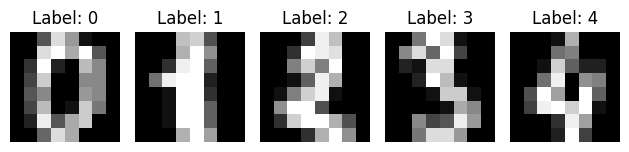
\includegraphics[width=.9\textwidth]{img/digits-vis.png}
    \caption[Five samples from the Digits dataset]{Five $8 \times 8$ samples from the Digits dataset with brightness levels from $0$ to $16$. Correct labels are shown above.}
    \label{fig:digits-vis}
\end{figure}

\paragraph{Preprocessing and input format}
This task involves multiclass classification ($y$: $[0,1,\dots,9]$). Because the input vectors contain features with multiple possible values, they must be transformed into a binary format compatible with the Tsetlin Machine. We achieved this using Scikit-learn's \texttt{OneHotEncoder}, which expanded the feature set from $X$: $(1797, 64)$ with values in $[0,1,\dots,16]$ to $X$: $(1797, 890)$ with binary values $[0,1]$. The data was divided using a typical $80\%$ training and $20\%$ testing split while maintaining class proportions.

\paragraph{Model hyperparameters}
Similar to the Noisy-XOR evaluation, we maintained default parameters while only modifying the \texttt{GridSearchCV} space for our classifier, as shown in Table~\ref{tab:digits-params}. Given the significantly higher number of features in this dataset, the parameter search determined that increasing the number of clauses to $1500$ was beneficial for performance.

\paragraph{Results and comparison}
The results summarized in Table~\ref{tab:digits-results} demonstrate that Tsetlin Machine models can handle more complex datasets. However, because the input format is restricted to binary, the models require a higher number of clauses to capture relevant patterns. This requirement leads to an increase in both time and memory consumption compared to other models. These findings suggest that the binary preprocessing required for TMs may not be ideal for high-dimensional image recognition tasks. Regardless, our implementation maintained accuracy levels comparable to the \GreenTsetlinName library, likely confirming the correctness of our implementation. Slightly longer training and prediction time are likely the result of \LibraryName not implementing vectorization, as decided in the design (see Section~\ref{sec:design}).

\begin{table}[!htbp]
\centering
\caption[Digits hyperparameters]{Hyperparameters and \texttt{GridSearchCV} search spaces for the Digits dataset. The table lists only parameters that differ from model defaults; for \texttt{GridSearchCV} the best-performing configuration is indicated in \texttt{\textbf{\underline{bold}}}\label{tab:digits-params}.}
\begin{tabularx}{\textwidth}{@{}l L@{}} \toprule
    \textbf{Model} & \textbf{Modified Parameters} \\ \midrule \midrule
    \texttt{Logistic Regression} & \texttt{max\_iter=1000} \\ \midrule
    \texttt{Decision Tree} & \texttt{---} \\ \midrule
    \texttt{Random Forest} & \texttt{---} \\ \midrule
    \texttt{MLP} & \texttt{max\_iter=1000, solver="lbfgs"} \\ \midrule
    \texttt{SVC} & \texttt{---} \\ \midrule
    \texttt{Linear SVC} & \texttt{dual="auto"} \\ \midrule
    \texttt{K-Nearest Neighbors} & \texttt{---} \\ \midrule
    \texttt{Gaussian Naive Bayes} & \texttt{---} \\ \midrule
    \texttt{Gradient Boosting} & \texttt{---} \\ \midrule
    \texttt{LightGBM} & \texttt{---} \\ \midrule
    \texttt{GridSearch Random Forest} & \texttt{n\_estimators: [50, 100, \textbf{\underline{200}}], max\_depth: [None, 10, 20, \textbf{\underline{30}}], min\_samples\_split: [\textbf{\underline{2}}, 5, 10]} \\ \midrule
    \texttt{GridSearch MLP} & \texttt{hidden\_layer\_sizes: [(50,), \textbf{\underline{(100,)}}, (50, 50)], activation: ["relu", \textbf{\underline{"tanh"}}], alpha: [0.0001, 0.001, \textbf{\underline{0.01}}]} \\ \midrule \midrule
    \texttt{Green Tsetlin} & \texttt{---}\\ \midrule
    \texttt{Green Tsetlin Sparse} & \texttt{---} \\ \midrule
    \texttt{C Tsetlin} & \texttt{---} \\ \midrule
    \texttt{GridSearch C Tsetlin} & \texttt{boost\_true\_positive\_feedback: [\textbf{\underline{False}}, True], num\_clauses: [500, 1000, \textbf{\underline{1500}}], s: [\textbf{\underline{3}}, 9]} \\ \midrule
    \texttt{C Tsetlin Sparse} & \texttt{---} \\ \midrule
    \texttt{GridSearch C Tsetlin Sparse} & \texttt{boost\_true\_positive\_feedback: [\textbf{\underline{False}}, True], num\_clauses: [64, 125, 500, \textbf{\underline{1000}}], s: [3, \textbf{\underline{9}}]} \\ \bottomrule
\end{tabularx}
\end{table}

\begin{table}[!htbp]
\centering
\setlength{\tabcolsep}{4pt}
\renewcommand{\arraystretch}{0.85}
\setlength{\aboverulesep}{2pt}
\setlength{\belowrulesep}{2pt}
\caption[Digits dataset benchmark results]{Benchmark results for the Digits dataset (evaluated on the Host (PC) environment). Model sizes are estimated based on internal data structures for Tsetlin-based models and via \texttt{pickle} exports for standard models, requiring caution when comparing directly. The best results are indicated in \texttt{\textbf{\underline{bold}}}\label{tab:digits-results}.}
\begin{tabularx}{\textwidth}{@{}l c c c c c r@{}} \toprule
    \textbf{\makecell[l]{Model}} & \textbf{\makecell[l]{Train\\Acc.}} & \textbf{\makecell[l]{Test\\Acc.}} & \textbf{\makecell[l]{Train\\Time (s)}} & \textbf{\makecell[l]{Train\\Pred.\\Time (s)}} & \textbf{\makecell[l]{Test\\Pred.\\Time (s)}} & \textbf{\makecell[l]{Model\\Size (B)}} \\ \midrule
    \texttt{\makecell[l]{Logistic Regression}} & \texttt{\textbf{\underline{1.0000}}} & \texttt{0.9528} & \texttt{1.5764} & \texttt{\textbf{\underline{0.0035}}} & \texttt{0.0042} & \texttt{84,514} \\
    \texttt{\makecell[l]{Decision Tree}} & \texttt{\textbf{\underline{1.0000}}} & \texttt{0.7833} & \texttt{0.0472} & \texttt{0.0038} & \texttt{\textbf{\underline{0.0024}}} & \texttt{\textbf{\underline{59,928}}} \\
    \texttt{\makecell[l]{Random Forest}} & \texttt{\textbf{\underline{1.0000}}} & \texttt{0.9444} & \texttt{0.2000} & \texttt{0.0159} & \texttt{0.0068} & \texttt{9,855,780} \\
    \texttt{\makecell[l]{MLP}} & \texttt{\textbf{\underline{1.0000}}} & \texttt{0.9306} & \texttt{4.5576} & \texttt{0.0226} & \texttt{0.0338} & \texttt{1,461,199} \\
    \texttt{\makecell[l]{SVC}} & \texttt{0.9965} & \texttt{\textbf{\underline{0.9583}}} & \texttt{0.2974} & \texttt{0.3944} & \texttt{0.1206} & \texttt{9,585,426} \\
    \texttt{\makecell[l]{Linear SVC}} & \texttt{\textbf{\underline{1.0000}}} & \texttt{0.9472} & \texttt{0.1006} & \texttt{0.0137} & \texttt{0.0068} & \texttt{84,395} \\
    \texttt{\makecell[l]{K-Nearest Neighbors}} & \texttt{0.9088} & \texttt{0.8667} & \texttt{\textbf{\underline{0.0028}}} & \texttt{0.0679} & \texttt{0.0101} & \texttt{10,256,123} \\
    \texttt{\makecell[l]{Gaussian Naive Bayes}} & \texttt{0.9666} & \texttt{0.8278} & \texttt{0.0062} & \texttt{0.0219} & \texttt{0.0052} & \texttt{155,647} \\
    \texttt{\makecell[l]{Gradient Boosting}} & \texttt{\textbf{\underline{1.0000}}} & \texttt{0.9139} & \texttt{9.5533} & \texttt{0.0150} & \texttt{0.0053} & \texttt{1,359,941} \\
    \texttt{\makecell[l]{LightGBM}} & \texttt{\textbf{\underline{1.0000}}} & \texttt{0.9472} & \texttt{0.6413} & \texttt{0.0092} & \texttt{0.0031} & \texttt{3,124,964} \\
    \texttt{\makecell[l]{GS Random Forest}} & \texttt{\textbf{\underline{1.0000}}} & \texttt{0.9444} & \texttt{5.6181} & \texttt{0.0347} & \texttt{0.0139} & \texttt{19,661,484} \\
    \texttt{\makecell[l]{GS MLP}} & \texttt{\textbf{\underline{1.0000}}} & \texttt{0.9361} & \texttt{8.0691} & \texttt{0.0346} & \texttt{0.0080} & \texttt{1,465,209} \\ \midrule
    \texttt{\makecell[l]{Green Tsetlin}} & \texttt{0.9923} & \texttt{0.9222} & \texttt{1.8070} & \texttt{0.0181} & \texttt{0.0063} & \texttt{1,794,040} \\
    \texttt{\makecell[l]{Green Tsetlin Sparse}} & \texttt{0.9402} & \texttt{0.8889} & \texttt{16.0517} & \texttt{0.0113} & \texttt{0.0042} & \texttt{822,040} \\
    \texttt{\makecell[l]{C Tsetlin}} & \texttt{0.9882} & \texttt{0.9222} & \texttt{18.6141} & \texttt{0.7369} & \texttt{0.1846} & \texttt{1,831,040} \\
    \texttt{\makecell[l]{GS C Tsetlin}} & \texttt{0.9937} & \texttt{0.9139} & \texttt{121.3198} & \texttt{1.0595} & \texttt{0.2674} & \texttt{2,746,540} \\
    \texttt{\makecell[l]{C Tsetlin Sparse}} & \texttt{0.6715} & \texttt{0.5972} & \texttt{21.0368} & \texttt{0.3977} & \texttt{0.1014} & \texttt{970,992} \\
    \texttt{\makecell[l]{GS C Tsetlin Sparse}} & \texttt{0.8045} & \texttt{0.7083} & \texttt{49.0949} & \texttt{0.3634} & \texttt{0.0939} & \texttt{967,712} \\ \bottomrule
\end{tabularx}
\end{table}

\clearpage
\section{Fashion-MNIST Dataset}
The Fashion-MNIST dataset~\cite{xiao2017/online} is a popular image classification task developed as a drop-in replacement for the original MNIST dataset. We utilized this dataset to test the performance limits and scaling capabilities of the Tsetlin Machine, as it is more difficult compared to the Digits dataset. This evaluation is conducted primarily for research purposes as we do not expect our implementation to be used in this types of task otherwise.

\paragraph{Dataset and problem representation}
The dataset consists of $70000$ grayscale images of Zalando's clothing articles. Each example is a $28 \times 28$ pixel image (brightness levels $0$-$255$) associated with one of the $10$ classes. Sample images from the dataset are illustrated in Figure~\ref{fig:fmnist-vis}.

\begin{figure}[!htbp]
    \centering
    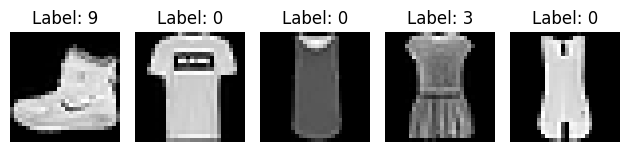
\includegraphics[width=.9\textwidth]{img/fmnist-vis.png}
    \caption[Five samples from the Fashion-MNIST dataset]{Five $28 \times 28$ samples from the Fashion-MNIST dataset with brightness levels from $0$ to $255$ before preprocessing. Correct labels are shown above.}
    \label{fig:fmnist-vis}
\end{figure}

\paragraph{Preprocessing and input format}
To prepare the data for the TM, we selected a subset consisting of the first $10000$ samples. The pixel values were normalized using the division by $16$ and cast to unsigned $8$-bit integers. The original resolution was down-sampled to $14 \times 14$ by selecting every second pixel in both dimensions. These images were then flattened into vectors of $196$ features. Since TMs require binary input, these features were transformed using Scikit-learn's \texttt{OneHotEncoder} with a maximum of $8$ categories. This process transformed the input dimensionality from $X$: $(10000, 784)$ with values in $[0,1,\dots,255]$ to $X$: $(10000, 1555)$ binary features. Finally, the data was divided into $80\%$ training and $20\%$ testing sets while maintaining the class proportions.

\paragraph{Model hyperparameters}
Due to the significant increase in training times with this dataset, we restricted the baseline models only to the Support Vector Classifier (\texttt{SVC}), which is a common method in image recognition tasks. As shown in Table~\ref{tab:f-mnist-params}, all the models evaluated were kept at their default parameter values.

\begin{table}[!htbp]
\centering
\caption[Fashion-MNIST hyperparameters]{Hyperparameters for the Fashion-MNIST dataset. The table lists only parameters that differ from model defaults\label{tab:f-mnist-params}.}
\begin{tabularx}{\textwidth}{@{}l L@{}} \toprule
    \textbf{Model} & \textbf{Modified Parameters} \\ \midrule \midrule
    \texttt{SVC} & \texttt{---} \\ \midrule \midrule
    \texttt{Green Tsetlin} & \texttt{---} \\ \midrule
    \texttt{Green Tsetlin Sparse} & \texttt{---} \\ \midrule
    \texttt{C Tsetlin} & \texttt{---} \\ \midrule
    \texttt{C Tsetlin Sparse} & \texttt{---} \\ \bottomrule
\end{tabularx}
\end{table}

\paragraph{Results and comparison}
The results in Table~\ref{tab:f-mnist-results} indicate that this dataset contains too many features for the current binary approach to TMs to remain efficient. This reveals a limitation in scaling, as all processing times increase significantly. Although both training and testing accuracy were lower than those of the \texttt{SVC}, prediction times for TM-based models remained faster. In particular, our implementation took significantly longer processing times than the \GreenTsetlinName library across all metrics. These findings suggest that the increase in dimensionality and the number of training samples creates performance bottlenecks that are more pronounced in our current implementation than in existing third-party libraries, likely because \LibraryName does not implement vectorization, as decided in the design (see Section~\ref{sec:design}).

\begin{table}[!htbp]
\centering
\setlength{\tabcolsep}{4pt}
\renewcommand{\arraystretch}{0.85}
\setlength{\aboverulesep}{2pt}
\setlength{\belowrulesep}{2pt}
\caption[Fashion-MNIST benchmark results]{Benchmark results for the Fashion-MNIST dataset (evaluated on the Host (PC) environment). Model sizes are estimated based on internal data structures for Tsetlin-based models and via \texttt{pickle} exports for standard models, requiring caution when comparing directly. The best results are indicated in \texttt{\textbf{\underline{bold}}}\label{tab:f-mnist-results}.}
\begin{tabularx}{\textwidth}{@{}l c c c c c r@{}} \toprule
    \textbf{\makecell[l]{Model}} & \textbf{\makecell[l]{Train\\Acc.}} & \textbf{\makecell[l]{Test\\Acc.}} & \textbf{\makecell[l]{Train\\Time (s)}} & \textbf{\makecell[l]{Train\\Pred.\\Time (s)}} & \textbf{\makecell[l]{Test\\Pred.\\Time (s)}} & \textbf{\makecell[l]{Model\\Size (B)}} \\ \midrule
    \texttt{\makecell[l]{SVC}} & \texttt{\textbf{\underline{0.9329}}} & \texttt{\textbf{\underline{0.8260}}} & \texttt{\textbf{\underline{8.3000}}} & \texttt{32.5356} & \texttt{8.2058} & \texttt{66,885,009} \\ \midrule
    \texttt{\makecell[l]{Green Tsetlin}} & \texttt{0.8053} & \texttt{0.7785} & \texttt{15.9906} & \texttt{\textbf{\underline{0.0475}}} & \texttt{\textbf{\underline{0.0136}}} & \texttt{3,124,040} \\
    \texttt{\makecell[l]{Green Tsetlin Sparse}} & \texttt{0.6094} & \texttt{0.5965} & \texttt{201.6389} & \texttt{0.0518} & \texttt{0.0151} & \texttt{\textbf{\underline{822,040}}} \\
    \texttt{\makecell[l]{C Tsetlin}} & \texttt{0.7600} & \texttt{0.7320} & \texttt{209.8398} & \texttt{6.5704} & \texttt{1.6151} & \texttt{3,161,040} \\
    \texttt{\makecell[l]{C Tsetlin Sparse}} & \texttt{0.5821} & \texttt{0.5810} & \texttt{633.4991} & \texttt{3.1626} & \texttt{0.7933} & \texttt{1,271,776} \\ \bottomrule
\end{tabularx}
\end{table}

\clearpage
\section{Incremental Noisy-XOR Learning}
The performance of Tsetlin Machines is highly sensitive to hyperparameter selection, which is often counter-intuitive. This marks the importance of performing an optimal configuration search using tools such as Grid Search. In this section, we evaluate the learning behavior of our model across sequential data batches to understand how specific impact incremental learning.

The training and testing accuracy curves per batch are illustrated in Figure~\ref{fig:noisy-xor-grid}. A comparison between models with different clause counts demonstrated that using $1000$ clauses allows the model to learn faster and achieve higher stability compared to using only $100$ clauses. This behavior shown in Figures~\ref{fig:noisy-xor-100-1}~and~\ref{fig:noisy-xor-1000-1} suggests that a larger pool of clauses may allow individual units to ``catch up'' to patterns more quickly.

The experimental results presented in Figures~\ref{fig:noisy-xor-1000-1}~and~\ref{fig:noisy-xor-1000-10} indicate that while increasing the number of epochs per batch improves accuracy on the current batch, it leads to the degradation of previously learned patterns, resulting in worse overall performance. This drop in accuracy is likely a consequence of the TM's internal forgetting mechanism during feedback processing. This presents a challenge for incremental learning, where maintaining a balance between retaining knowledge and memorizing new patterns is crucial.

\begin{figure}[!htbp]
    \centering
    % Row 1, Left
    \begin{subfigure}{0.49\textwidth}
        \centering
        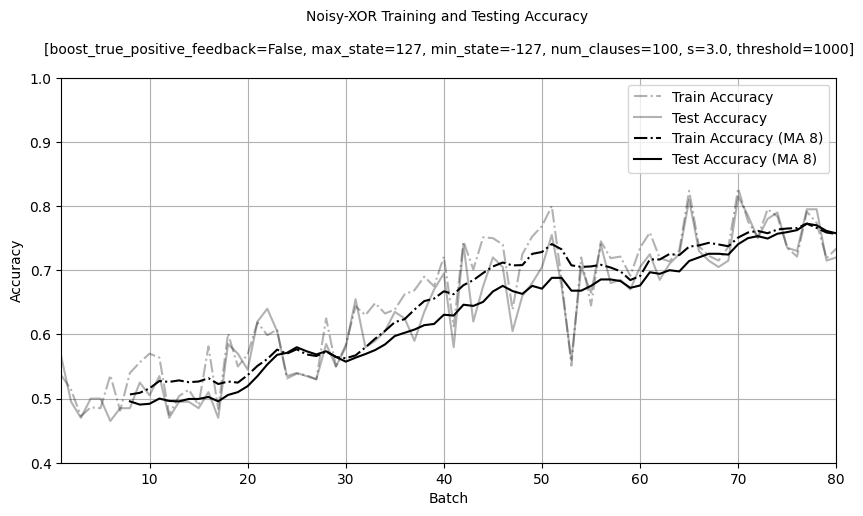
\includegraphics[width=\textwidth]{img/noisy-xor-100-clauses-1-epoch-per-batch.png}
        \caption{100 clauses, 1 epoch per batch}
        \label{fig:noisy-xor-100-1}
    \end{subfigure}
    \hfill
    % Row 1, Right
    \begin{subfigure}{0.49\textwidth}
        \centering
        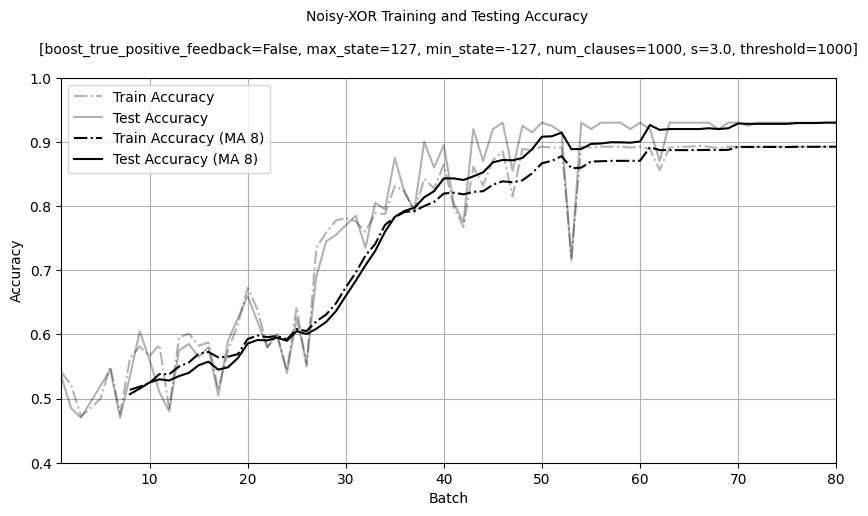
\includegraphics[width=\textwidth]{img/noisy-xor-1000-clauses-1-epoch-per-batch.png}
        \caption{1000 clauses, 1 epoch per batch}
        \label{fig:noisy-xor-1000-1}
    \end{subfigure}

    \vspace{1em}

    % Row 2, Left
    \begin{subfigure}{0.49\textwidth}
        \centering
        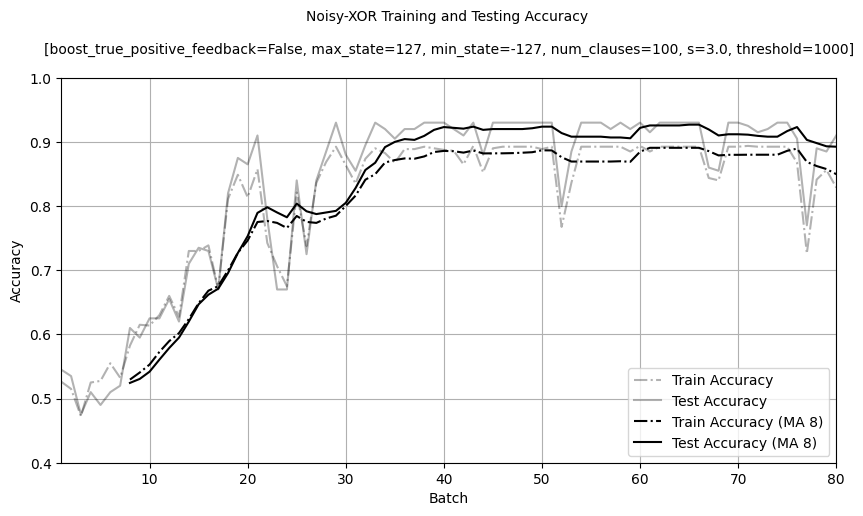
\includegraphics[width=\textwidth]{img/noisy-xor-100-clauses-10-epoch-per-batch.png}
        \caption{100 clauses, 10 epochs per batch}
        \label{fig:noisy-xor-100-10}
    \end{subfigure}
    \hfill
    % Row 2, Right
    \begin{subfigure}{0.49\textwidth}
        \centering
        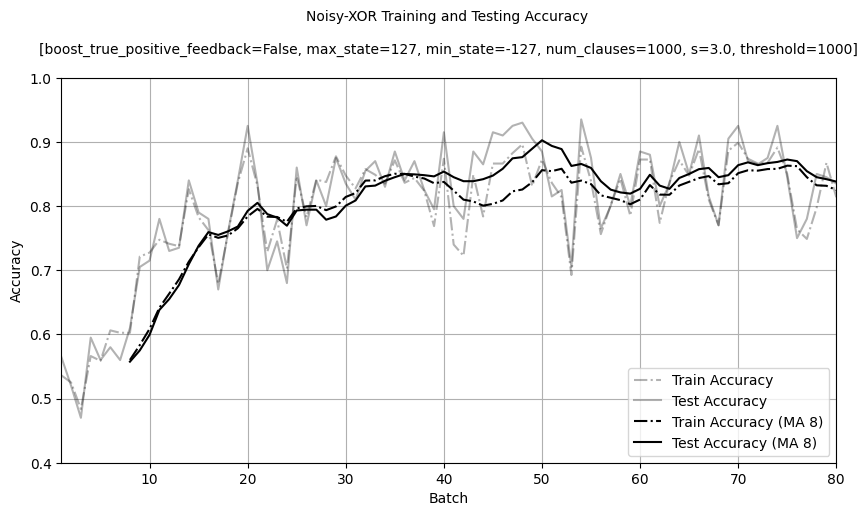
\includegraphics[width=\textwidth]{img/noisy-xor-1000-clauses-10-epoch-per-batch.png}
        \caption{1000 clauses, 10 epochs per batch}
        \label{fig:noisy-xor-1000-10}
    \end{subfigure}

    \caption[Train and test accuracy per batch on the Noisy-XOR]{Train accuracy (dash-dot line) and test accuracy (solid line) per batch for the Noisy-XOR dataset. The evaluation tracks progress over 80 batches of 10 samples each.}
    \label{fig:noisy-xor-grid}
\end{figure}

\clearpage
\section{Embedded Noisy-XOR Benchmarks}
We demonstrated the capability of our implementation by running the minimal version of the core C library on resource-constrained hardware. As a target platform, we chose the Raspberry Pi Pico development board due to its popularity and software support, specifically the Pico-SDK~\cite{pico-sdk}. The platform is powered by the RP2040 microcontroller chip, featuring a dual-core Arm Cortex-M0+ processor clocked at 133 MHz, 264 KB of SRAM and 2 MB of on-board flash memory.

We conducted benchmarks on the Noisy-XOR dataset similar to those performed in Python but using a wider range of configurations. Selected tests were performed on a desktop PC running Ubuntu OS in cases where the models exceeded the hardware performance limits of the Raspberry Pi Pico or where peak memory statistics were unavailable. The results are detailed in Table~\ref{tab:noisy-xor-pi-pico}, with values gathered from the Ubuntu environment marked with a \textbf{(U)} prefix.

The analysis reveals several important characteristics:
\begin{compactitem}
    \item Tsetlin Machine memory usage (\textbf{TMM}) is directly proportional only to the number of clauses.
    \item Training time (\textbf{TRT}) is proportional to the number of clauses, samples, and epochs.
    \item Evaluation time (\textbf{EVT}) is also proportional to the number of clauses, and samples.
    \item Other hyperparameters than mentioned above have a relatively small impact on performance when set to values close to established model defaults.
    \item Accurately measuring peak memory usage (\textbf{PMU}) proved difficult in the Ubuntu environment due to system overhead.
\end{compactitem}

As shown in Table~\ref{tab:noisy-xor-pi-pico}, our implementation remains highly usable on embedded hardware. For example, configurations \textbf{9} and \textbf{10} achieve accuracy levels close to the theoretical maximum (counting for the $10\%$ added noise). We can observe a clear trade-off: using more epochs and fewer clauses (Configuration \textbf{10}) results in a longer training time but a smaller memory footprint and faster prediction speeds, which is ideal for pretrained models. In contrast, using a single epoch with more clauses (Configuration \textbf{9}) allows faster on-device learning at the cost of increased model size and slower evaluation.

\begin{sidewaystable}[!htbp]
\centering
\scriptsize
\setlength{\tabcolsep}{2.5pt}
\caption[Noisy-XOR performance on Raspberry Pi Pico]{Noisy-XOR results on Raspberry Pi Pico and Ubuntu Desktop (the Host (PC) environment), testing how hyperparameters affect accuracy and execution time. Peak RAM usage was calculated on the Ubuntu Desktop and includes system overhead. Due to hardware performance limits, configurations exceeding the 1000 clauses were benchmarked only on Ubuntu (marked with \textbf{(U)} prefix)\label{tab:noisy-xor-pi-pico}.}
\begin{tabular}{@{}r r r r r r r r r r r r r r r r r r r r@{}} \toprule
    \textbf{N} & \textbf{SAM} & \textbf{CLS} & \textbf{THR} & \textbf{LIT} & \textbf{CLU} & \textbf{MXS} & \textbf{MNS} & \textbf{BST} & \textbf{SNS} & \textbf{EPC} & \textbf{TRT} & \textbf{EVT} & \textbf{COP} & \textbf{TOP} & \textbf{ACC} & \textbf{TMM} & \textbf{DSM} & \textbf{PMU} \\ \midrule
    1 & 1000 & 2 & 1000 & 16 & 1000 & 127 & -127 & 0 & 3.0 & 1 & 24.73 & 0.88 & 183 & 200 & 0.92 & 36.21 & 19.53 & \textbf{(U)}1728.0 \\
    2 & 1000 & 2 & 1000 & 16 & 1000 & 127 & -127 & 0 & 3.0 & 2 & 41.30 & 0.87 & 183 & 200 & 0.92 & 36.21 & 19.53 & \textbf{(U)}1728.0 \\
    3 & 1000 & 2 & 1000 & 16 & 1000 & 127 & -127 & 0 & 3.0 & 4 & 72.51 & 0.88 & 183 & 200 & 0.92 & 36.21 & 19.53 & \textbf{(U)}1728.0 \\
    4 & 1000 & 2 & 1000 & 16 & 1000 & 63 & -63 & 0 & 3.0 & 1 & 24.73 & 0.88 & 183 & 200 & 0.92 & 36.21 & 19.53 & \textbf{(U)}1728.0 \\
    5 & 1000 & 2 & 1000 & 16 & 1000 & 31 & -31 & 0 & 3.0 & 1 & 24.73 & 0.88 & 183 & 200 & 0.92 & 36.21 & 19.53 & \textbf{(U)}1728.0 \\
    6 & 1000 & 2 & 1000 & 16 & 1000 & 15 & -15 & 0 & 3.0 & 1 & 24.51 & 0.86 & 183 & 200 & 0.92 & 36.21 & 19.53 & \textbf{(U)}1728.0 \\
    7 & 1000 & 2 & 1000 & 16 & 500 & 127 & -127 & 0 & 3.0 & 1 & 12.92 & 0.40 & 183 & 200 & 0.92 & 18.15 & 19.53 & \textbf{(U)}1728.0 \\
    8 & 1000 & 2 & 1000 & 16 & 250 & 127 & -127 & 0 & 3.0 & 1 & 6.79 & 0.21 & 183 & 200 & 0.92 & 9.12 & 19.53 & \textbf{(U)}1728.0 \\
    \textbf{\underline{9}} & 1000 & 2 & 1000 & 16 & 125 & 127 & -127 & 0 & 3.0 & 1 & 3.54 & 0.10 & 183 & 200 & 0.92 & 4.6 & 19.53 & \textbf{(U)}1728.0 \\
    \textbf{\underline{10}} & 1000 & 2 & 1000 & 16 & 64 & 127 & -127 & 0 & 3.0 & 10 & 11.93 & 0.05 & 183 & 200 & 0.92 & 2.39 & 19.53 & \textbf{(U)}1728.0 \\
    11 & 1000 & 2 & 1000 & 16 & 1000 & 127 & -127 & 0 & 3.0 & 10 & 163.19 & 0.89 & 182 & 200 & 0.91 & 36.21 & 19.53 & \textbf{(U)}1728.0 \\
    12 & 1000 & 2 & 500 & 16 & 1000 & 127 & -127 & 0 & 3.0 & 1 & 22.98 & 0.87 & 182 & 200 & 0.91 & 36.21 & 19.53 & \textbf{(U)}1728.0 \\
    13 & 1000 & 2 & 1000 & 16 & 1000 & 127 & -127 & 1 & 3.0 & 1 & 24.53 & 0.82 & 181 & 200 & 0.91 & 36.21 & 19.53 & \textbf{(U)}1728.0 \\
    14 & 1000 & 2 & 250 & 16 & 1000 & 127 & -127 & 0 & 3.0 & 1 & 22.58 & 0.89 & 180 & 200 & 0.9 & 36.21 & 19.53 & \textbf{(U)}1728.0 \\
    15 & 1000 & 2 & 1000 & 16 & 1000 & 127 & -127 & 0 & 6.0 & 1 & 26.33 & 0.67 & 179 & 200 & 0.9 & 36.21 & 19.53 & \textbf{(U)}1728.0 \\
    16 & 1000 & 2 & 32 & 16 & 1000 & 127 & -127 & 0 & 3.0 & 1 & 21.30 & 0.87 & 179 & 200 & 0.9 & 36.21 & 19.53 & \textbf{(U)}1728.0 \\
    17 & 250 & 2 & 1000 & 16 & 1000 & 127 & -127 & 0 & 3.0 & 10 & 47.14 & 0.22 & 44 & 50 & 0.88 & 36.21 & 4.88 & \textbf{(U)}1728.0 \\
    18 & 1000 & 2 & 125 & 16 & 1000 & 127 & -127 & 0 & 3.0 & 1 & 21.54 & 0.88 & 173 & 200 & 0.87 & 36.21 & 19.53 & \textbf{(U)}1728.0 \\
    19 & 1000 & 2 & 64 & 16 & 1000 & 127 & -127 & 0 & 3.0 & 1 & 21.03 & 0.88 & 170 & 200 & 0.85 & 36.21 & 19.53 & \textbf{(U)}1728.0 \\
    20 & 1000 & 2 & 32 & 16 & 500 & 127 & -127 & 0 & 3.0 & 1 & 10.87 & 0.44 & 168 & 200 & 0.84 & 18.15 & 19.53 & \textbf{(U)}1728.0 \\
    21 & 1000 & 2 & 32 & 16 & 500 & 127 & -127 & 0 & 3.0 & 10 & 79.82 & 0.46 & 166 & 200 & 0.83 & 18.15 & 19.53 & \textbf{(U)}1728.0 \\
    22 & 1000 & 2 & 1000 & 16 & 1000 & 7 & -7 & 0 & 3.0 & 1 & 27.17 & 0.81 & 165 & 200 & 0.83 & 36.21 & 19.53 & \textbf{(U)}1728.0 \\
    23 & 1000 & 2 & 1000 & 16 & 64 & 127 & -127 & 0 & 3.0 & 1 & 1.85 & 0.05 & 162 & 200 & 0.81 & 2.39 & 19.53 & \textbf{(U)}1728.0 \\
    24 & 1000 & 2 & 16 & 16 & 1000 & 127 & -127 & 0 & 3.0 & 1 & 21.27 & 0.85 & 161 & 200 & 0.81 & 36.21 & 19.53 & \textbf{(U)}1728.0 \\
    25 & 500 & 2 & 1000 & 16 & 1000 & 127 & -127 & 0 & 3.0 & 1 & 36.21 & 0.44 & 80 & 100 & 0.8 & 36.21 & 9.77 & \textbf{(U)}1728.0 \\
    26 & 1000 & 2 & 32 & 16 & 500 & 127 & -127 & 1 & 3.0 & 1 & 10.74 & 0.42 & 150 & 200 & 0.75 & 18.15 & 19.53 & \textbf{(U)}1728.0 \\
    27 & 1000 & 2 & 1000 & 16 & 64 & 127 & -127 & 1 & 3.0 & 1 & 1.79 & 0.05 & 142 & 200 & 0.71 & 2.39 & 19.53 & \textbf{(U)}1728.0 \\
    28 & 1000 & 2 & 1000 & 16 & 1000 & 127 & -127 & 0 & 1.5 & 1 & 30.84 & 1.15 & 124 & 200 & 0.62 & 36.21 & 19.53 & \textbf{(U)}1728.0 \\
    29 & 250 & 2 & 1000 & 16 & 1000 & 127 & -127 & 0 & 3.0 & 1 & 7.21 & 0.22 & 27 & 50 & 0.54 & 36.21 & 4.88 & \textbf{(U)}1728.0 \\
    30 & 1000 & 2 & 1000 & 16 & 1000 & 3 & -3 & 0 & 3.0 & 1 & 28.43 & 0.73 & 100 & 200 & 0.5 & 36.21 & 19.53 & \textbf{(U)}1728.0 \\
    31 & 1000 & 2 & 1000 & 16 & 10000 & 127 & -127 & 0 & 3.0 & 1 & \textbf{(U)}1.16 & \textbf{(U)}0.11 & 172 & 200 & 0.86 & 361.45 & 19.53 & \textbf{(U)}2112.0 \\
    32 & 1000 & 2 & 1000 & 16 & 100000 & 127 & -127 & 0 & 3.0 & 1 & \textbf{(U)}11.61 & \textbf{(U)}1.17 & 167 & 200 & 0.84 & 3613.4 & 19.53 & \textbf{(U)}5376.0 \\
    33 & 1000 & 2 & 1000 & 16 & 200000 & 127 & -127 & 0 & 3.0 & 1 & \textbf{(U)}23.00 & \textbf{(U)}2.32 & 165 & 200 & 0.83 & 7226.68 & 19.53 & \textbf{(U)}8832.0 \\ \bottomrule
\end{tabular}
\vspace{1ex}
\begin{flushleft}
\textbf{Legend:} 
\textbf{N}:~Configuration Number,
\textbf{SAM}:~Number of Samples, 
\textbf{CLS}:~Number of Classes, 
\textbf{THR}:~Threshold, 
\textbf{LIT}:~Number of Literals, 
\textbf{CLU}:~Number of Clauses, 
\textbf{MXS}:~Maximum State,
\textbf{MNS}:~Minimum State,
\textbf{BST}:~Boost True Positive Feedback,
\textbf{SNS}:~Learning Sensitivity (s),
\textbf{EPC}:~Training Epochs,
\textbf{TRT}:~Training Time [s],
\textbf{EVT}:~Evaluation Time [s],
\textbf{COP}:~Correct Predictions,
\textbf{TOP}:~Total Predictions,
\textbf{ACC}:~Accuracy,
\textbf{TMM}:~TM Memory Usage [KB],
\textbf{DSM}:~Dataset Memory Usage (\texttt{static}) [KB],
\textbf{PMU}:~Peak Memory Usage on Ubuntu Desktop [KB]
\end{flushleft}
\end{sidewaystable}

\clearpage
\section{Summary}
The initial evaluation of our Tsetlin Machine implementations shows potential, especially for resource-limited environments dealing with not overly high-dimensional data. We observed the impact of hyperparameters, mainly number of clauses and training epochs, making it essential to tune them for each task. We observed the mechanism inside TM designed to prevent overfitting, creating a challenge in incremental learning, where the balance between retaining old knowledge and memorizing new patterns is crucial. Furthermore, benchmarking was complicated due to the \GreenTsetlinName library design, which includes some undocumented optimizations (e.g. \texttt{literal\_budget} parameter that is not properly described).
\chapter{Conclusions}
\label{chap:conclusions}

The previous chapters have described the goals of the project. This concluding chapter reflects on the objectives that were achieved successfully and identifies any areas of improvement. It also proposes further work, research and improvements to the project as well as TMs in general.

\section{Achieved Results}
The project work resulted in a functional, stable and optimized open-source product, pending only cosmetic or experiential refinements. All base requirements were fulfilled -- the Tsetlin Machine execution engine can be used to both infer and train in a limited resource environment, model data is stored in an efficient, easy to utilize format. The project further mitigates a gap in the ecosystem encountered during its development -- the lack of available knowledge sources and documentation on how to put the TM theory into practice. The product is suitable for production use, though compilation for non-standard or specialized architectures requires additional effort.

\section{Further Work}
During the development period of the project, numerous promising ideas emerged that warrant further investigation. These ideas merit further investigation and could meaningfully enhance both the research outcomes and the overall robustness of the project.

\subsection{Cross Compilation}
An immediate extension that would increase the utility and reach of this project is the introduction of a formal cross-compilation pipeline. Implementing cross-compilation would enable automated builds for multiple target architectures (e.g. ARM, RISC-V, x86\_64) and ABIs, improving portability and facilitating deployment on embedded and heterogeneous systems. Addressing this would broaden its applicable use cases.

\subsection{Coalesced TM and the Linear Layer}
Seeing the similarities between TM and a Perceptron~\cite{sharma2022equivalenceweightedtsetlinmachine}, further parallels could be drawn between a Coalesced TM and a whole Linear layer and activation function of a Neural Network. More research is necessary to find out whether they could be used interchangeably. Likely results would vary a lot based on task complexity and data structure. Another idea to explore is whether TMs could be combined sequentially with creating a larger model, with or without other layer types.

Due to how customizable \LibraryName is, a custom feedback function and output activation function can be written to facilitate a TM to be used as a layer of a larger model -- painlessly, without the need to rewrite the main logic of the execution engine.

\subsection{Integer Only Implementation of TM}
Some processors and compute units do not natively provide a floating-point unit, especially on embedded systems and similar hardware. TM design typically requires floating point operations, however authors believe it should not be difficult to implement.

All floating point operations in TM design originate from the parameter \textit{s} -- learning sensitivity -- which handles how often specific feedback types should apply. This is traditionally done using floating point, however rewriting this behavior to integer-only logic seems rather straightforward.
 %%%%%%%%%%%%%%%%%%%%%%%%%%%%%%%%%%%%%
 %%%%%%%%%%%%%%%%%%%%%%%%%%%%%%%%%%%%%
\appendix % Dodatek
 %%%%%%%%%%%%%%%%%%%%%%%%%%%%%%%%%%%%%
 % Rozdziały dodatku
% \chapter{Typowe elementy składowe pracy dyplomowej z informatyki}
\section{Tabele}
\begin{comment}
    \begin{itemize}
        \item Każda tabela powinna być opisana w treści pracy.
        \item Podpis ma być przed tabelą.
    \end{itemize}
\end{comment}
W tabeli \ref{tab:result} przedstawiono wyniki pomiarów.
\begin{table}[!h]
    \caption{Pomiary zużycia energii elektrycznej\label{tab:result}.}
    \centering
    \begin{tabular}{|l||r@{,}l|}
        \hline
        \textbf{L.p.} & \multicolumn{2}{|c|}{\textbf{Wartość}}          \\
        \hline
        \hline
        \cline{2-3}
        %\textbf{L.p.} & \multicolumn{1}{r@{\,\vline\,}}{Całkowita} & Ułamkowa \\
        \hline
        1             & 12345                                  & 6789   \\
        \cline{2-3}
                      & 45                                     & 89     \\
        \hline
        2             & 45                                     & 678901 \\
        \hline
    \end{tabular}
\end{table}

Jeżeli tabela zawiera dużą liczbę wierszy i może nie zmieścić się na stronie \pauza patrz tabela \ref{tab:longtable} \pauza skorzystaj z pakietu \emph{longtable} \cite{longtable}.
\begin{longtable}{|p{14ex}|p{1.5em}|p{1.5em}|p{1.5em}|p{1.5em}|p{1.5em}|p{1.5em}|p{1.5em}|p{1.5em}|p{1.5em}|}
    \caption{Tabela, która zawiera dużą liczbę wierszy\label{tab:longtable}.}
    \endfirsthead
    \hline
               & 1 & 2 & 3 & 4 & 5 & 6 & 7 & 8 & \\
    \cline{2-9}
               &   &   &   &   &   &   &   &   & \\
    \hline
    \endhead
    \endfoot
    \hline\hline
               & 1 & 2 & 3 & 4 & 5 & 6 & 7 & 8 & \\
    \cline{2-9}
               &   &   &   &   &   &   &   &   & \\
    \hline\hline
    Student 1  &   &   &   &   &   &   &   &   & \\
    \cline{2-9}
               &   &   &   &   &   &   &   &   & \\
    \hline\hline
    Student 2  &   &   &   &   &   &   &   &   & \\
    \cline{2-9}
               &   &   &   &   &   &   &   &   & \\
    \hline\hline
    Student 3  &   &   &   &   &   &   &   &   & \\
    \cline{2-9}
               &   &   &   &   &   &   &   &   & \\
    \hline\hline
    Student 4  &   &   &   &   &   &   &   &   & \\
    \cline{2-9}
               &   &   &   &   &   &   &   &   & \\
    \hline\hline
    Student 5  &   &   &   &   &   &   &   &   & \\
    \cline{2-9}
               &   &   &   &   &   &   &   &   & \\
    \hline\hline
    Student 6  &   &   &   &   &   &   &   &   & \\
    \cline{2-9}
               &   &   &   &   &   &   &   &   & \\
    \hline\hline
    Student 7  &   &   &   &   &   &   &   &   & \\
    \cline{2-9}
               &   &   &   &   &   &   &   &   & \\
    \hline\hline
     Student 8  &   &   &   &   &   &   &   &   & \\
     \cline{2-9}
                &   &   &   &   &   &   &   &   & \\
     \hline\hline
     Student 9  &   &   &   &   &   &   &   &   & \\
    \cline{2-9}
                &   &   &   &   &   &   &   &   & \\
    \hline\hline
    % Student 10 &   &   &   &   &   &   &   &   & \\
    % \cline{2-9}
    %            &   &   &   &   &   &   &   &   & \\
    % \hline\hline
    % Student 11 &   &   &   &   &   &   &   &   & \\
    % \cline{2-9}
    %            &   &   &   &   &   &   &   &   & \\
    % \hline\hline
    % Student 12 &   &   &   &   &   &   &   &   & \\
    % \cline{2-9}
    %            &   &   &   &   &   &   &   &   & \\
    % \hline\hline
    % Student 13 &   &   &   &   &   &   &   &   & \\
    % \cline{2-9}
    %            &   &   &   &   &   &   &   &   & \\
    % \hline\hline
\end{longtable}

Tabele, w których występuje długi tekst, a co za tym idzie może się on nie zmieścić \pauza musi zostać zawinięty, z pomocą przychodzi środowisko 'tabularx' \cite{tabularx} \pauza  patrz tabela \ref{tab:tabularx}.
\begin{table}[!ht]
    \caption{Tabela zawierająca długi tekst\label{tab:tabularx}.}
    \centering
    \begin{tabularx}{300pt}{|c|X|c|X|}
        \hline
        \multicolumn{2}{|c|}{Wpis wielokolumnowy!} &
        TRZY                                       &
        CZTERY                                       \\
        \hline
        jeden                                      &
        \raggedright\arraybackslash Szerokość tej kolumny zależy od
        szerokości tabeli.                         &
        trzy                                       &
        \raggedright\arraybackslash Kolumna czwarta będzie zachowywać się w taki sam sposób jak
        druga kolumna o tej samej szerokości.        \\
        \hline
    \end{tabularx}
\end{table}
 %%%%%%%%%%%%%%%%%%%%%%%%%%%%%%%%%%%%%
\section{Rysunki}
\begin{comment}  
    \begin{itemize}
        \item Rysunki powinny być przerysowane samodzielnie albo używane tylko te,
          których twórcy zezwolili na ich rozpowszechnianie oraz kopiowanie, czyli
          np. rysunki objęte licencją Creative Commons.
        \item Każdy rysunek powinien być opisany w treści pracy.
    \end{itemize}
\end{comment}
\subsection{Wewnętrzne}
Klasa \emph{agh-wi}, automatycznie, dołącza pakiet \emph{TikZ} \cite{tikz} \pauza dostarcza on komend pozwalających na tworzenie grafik. Przykładowe grafiki pokazano na rysunku \ref{fig:tikz1} oraz \ref{fig:tikz2}.
 %%%%%%%%%%%%%%%%%
\begin{figure}[!h]
    \begin{center}
        \tikz \draw[thick,rounded corners=8pt]
        (0,0) -- (0,2) -- (1,3.25) -- (2,2) -- (2,0) -- (0,2) -- (2,2) -- (0,0) -- (2,0);
    \end{center}
    \caption{Prosty rysunek \emph{TikZ}\label{fig:tikz1}.}
\end{figure}
 %%%%%%%%%%%%%%%%%
\begin{figure}[!ht]
    \begin{center}
        \begin{tikzpicture}
            \draw[step=.5cm,gray,very thin] (-1.4,-1.4) grid (1.4,1.4);
            \draw (-1.5,0) -- (1.5,0);
            \draw (0,-1.5) -- (0,1.5);
            \draw (0,0) circle [radius=1cm];
        \end{tikzpicture}
    \end{center}
    \caption{Bardziej złożony rysunek \emph{TikZ}\label{fig:tikz2}.}
\end{figure}
 %%%%%%%%%%%%%%%%%

Oprócz rysunków eksponowanych możliwe jest tworzenie grafik będących  \tikz{\fill[orange] (0ex,0ex) circle (1ex);  \fill[red] (1ex,1ex) circle (1ex);} częścią \tikz{\draw (0pt,0pt) -- (20pt,6pt);} zdania. 

\emph{TikZ} pozwala również na kreślenie po powierzchni strony, np. możemy narysować strzałki pomiędzy elementami strony.
\begin{shaded}
 %%%%%%%%%%%%%%%%%%%%%%%%%%%%%%%%%%%%%%%%%%%%%%%%%%%
 % Zmodyfikowana wersja przykładu ze strony  https://texample.net/tikz/examples/global-nodes/
 %%%%%%%%%%%%%%%%%%%%%%%%%%%%%%%%%%%%%%%%%%%%%%%%%%%
Ułamek \pauza patrz wzór \ref{eqn:tikz} \pauza składa się z: 
\begin{itemize}
    \item Licznika \tikz[na] \node (n1) {};
\end{itemize}
 %%%%%%%%%%%%%%%%%
\begin{equation}
    a =  \frac{\tikz[baseline] \node[fill=blue!20,rectangle] (t1){$x+y$};}{\tikz[baseline] \node[fill=red!20, ellipse] (t2){$y-z$}; }
    \label{eqn:tikz}
\end{equation}
 %%%%%%%%%%%%%%%%%
\begin{itemize}
    \item Mianownika \tikz\node[na] (n2) {};
\end{itemize}
 %%%%%%%%%%%%%%%%%
\begin{tikzpicture}[overlay]
    \path  (n1) edge [->,bend left] (t1);
    \path  (n2) edge [->,bend right] (t2);
\end{tikzpicture}
\end{shaded}
\subsection{Zewnętrzne}
Oczywiście możliwe jest również dołączanie rysunków zewnętrznych \pauza
pakiet \emph{graphicx} \cite{graphicx} pozwala na wstawianie grafik zapisanych w  plikach: '.png', '.jpg' oraz '.pdf'. Rysunek \ref{fig:logo} wstawiono przy użyciu tego pakietu.
\begin{figure}[!ht]
    \begin{center}
        \IfFileExists{img/logo_podstawowe.png}{
            
\includegraphics[width=0.7\linewidth]{img/logo_podstawowe}
        }
        {Nie znaleziono pliku 'img/logo\_podstawowe.png' \pauza pobierz go ze strony \url{https://www.informatyka.agh.edu.pl/media/uploads/Logo WI/PNG/logo_podstawowe.png}}
    \end{center}
    \caption{Logo Wydziału Informatyki.}
    \label{fig:logo}
\end{figure}
  %%%%%%%%%%%%%%%%%%%%%%%%%%%%%%%%%%%%%
\section{Kody źródłowe}
Najpopularniejszymi pakietami, które umożliwiają składanie kodów źródłowych programów, są:
\begin{description}
    \item[listings \cite{listings}] \pauza kod źródłowy jest formatowany bezpośrednio przez \LaTeX{}\dywiz{}a \pauza nie jest używany żaden, zewnętrzny, formater kodu.
        \begin{lstlisting}[language=C++, float=ht, label=lst:code1, caption={Przykładowy kod źródłowy sformatowany za pomocą pakietu 'listings'.}]
/* Pierwszy program w C++ */

#include <iostream>

int main() {
    std::cout << "Hello World!";
    return 0;
}
    \end{lstlisting}
    \item[minted \cite{minted}] \pauza formatuje kod źródłowy przy użyciu biblioteki języka Python  o nazwie \emph{Pygments} \cite{pygments}.
        \begin{listing}[!ht]
            \caption{Przykładowy listing sformatowany za pomocą pakietu 'minted'.\label{lst:code2}}
            \begin{minted}{c++}
/* Pierwszy program w C++ */

#include <iostream>

int main() {
    std::cout << "Hello World!";
    return 0;
}
    \end{minted}
        \end{listing}
\end{description}

\begin{comment}
    \begin{itemize}
        \item Podpis ma być przed kodem źródłowym.
        \item \alert{Proszę używać tylko jednego z tych pakietów}; w przeciwnym razie otrzymasz taki efekt, jak w przykładowej pracy \pauza obydwa listingi mają ten sam numer.
    \end{itemize}
\end{comment}

Kod źródłowy w C++ sformatowany przy użyciu pakietu \emph{listings}, pokazano na listingu \ref{lst:code1}; sformatowany przy użyciu pakietu \emph{minted}, pokazano na listingu \ref{lst:code2}.
%%%%%%%%%%%%%%%%%%%%%%%%%%%%%%%%%%%%%
\section{Algorytmy}
Pakiet \emph{algorithm2e} \cite{algorithm2e} to jeden z kilku, które pozwalają zapisywać algorytmy w formie pseudokodu \pauza patrz
algorytm \ref{alg:algo_disjdecomp}.
\begin{comment}
    Podpis ma być przed algorytmem.
\end{comment}
\begin{algorithm}[!htb]
    \caption{Disjoint decomposition.}\label{alg:algo_disjdecomp}
    %%%%%%%%%%%%%%%%%%%%%%%%%%     
    \SetKwData{Left}{left}\SetKwData{This}{this}\SetKwData{Up}{up}
    \SetKwFunction{Union}{Union}\SetKwFunction{FindCompress}{FindCompress}
    \SetKwInOut{Input}{input}\SetKwInOut{Output}{output}
    \Input{A bitmap $Im$ of size $w\times l$}
    \Output{A partition of the bitmap}
    \BlankLine
    \emph{special treatment of the first line}\;
    \For{$i\leftarrow 2$ \KwTo $l$}{
        \emph{special treatment of the first element of line $i$}\;
        \For{$j\leftarrow 2$ \KwTo $w$}{\label{forins}
            \Left$\leftarrow$ \FindCompress{$Im[i,j-1]$}\;
            \Up$\leftarrow$ \FindCompress{$Im[i-1,]$}\;
            \This$\leftarrow$ \FindCompress{$Im[i,j]$}\;
            \If(\tcp*[h]{O(\Left,\This)==1}){\Left compatible with \This}{\label{lt}
                \lIf{\Left $<$ \This}{\Union{\Left,\This}}
                \lElse{\Union{\This,\Left}}
            }
            \If(\tcp*[f]{O(\Up,\This)==1}){\Up compatible with \This}{\label{ut}
                \lIf{\Up $<$ \This}{\Union{\Up,\This}}
                \tcp{\This is put under \Up to keep tree as flat as possible}\label{cmt}
                \lElse{\Union{\This,\Up}}\tcp*[h]{\This linked to \Up}\label{lelse}
            }
        }
        \lForEach{element $e$ of the line $i$}{\FindCompress{p}}
    }
\end{algorithm}\DecMargin{1em}
 %%%%%%%%%%%%%%%%%%%%%%%%%%%%%%%%%%%%%
\section{Wzory}
\LaTeX{} bardzo dobrze sprawdza się w przypadku prac dyplomowych zawierających wzory matematyczne\footnote{ W przypadku złożonych wzorów warto zastosować pakiet \emph{amsmath} \cite{amsmath}.}.
\subsection{Przykłady}
Wzór $E = mc^{2}$\nomenclature{$c$}{Prędkość światła w próżni} jest częścią zdania.

\begin{equation}
    \left|\sum_{i=1}^n a_ib_i\right|
    \le
    \left(\sum_{i=1}^n a_i^2\right)^{1/2}
    \left(\sum_{i=1}^n b_i^2\right)^{1/2}
\end{equation}

 % Do wstawienia poniższych wzorów użyto środowisk (otoczeń) zdefiniowanych w pakiecie 'amsmath'
Wartości zmiennej opisano wzorem \ref{eq:r1}.
\begin{equation}
    \label{eq:r1}
    x=\begin{cases}
        y           & \text{dla } y > 0    \\
        \frac{z}{y} & \text{dla } y \leq 0
    \end{cases}
\end{equation}

Wzór \ref{eq:r2} to wzór wielowierszowy.
\begin{align}
    \label{eq:r2}
    2x^2 + 3(x-1)(x-2) & =2x^2 + 3(x^2-3x+2)             \\
                       & = 2x^2 + 3x^2 - 9x + 6\nonumber \\
                       & = 5x^2 - 9x + 6\nonumber
\end{align}
\begin{comment}
    Należy używać tylko dwóch rodzajów wzorów:
    \begin{enumerate}
        \item \enquote{W linii}.
        \item Eksponowane, numerowane.
    \end{enumerate}
\end{comment}
 %%%%%%%%%%%%%%%%%%%%%%%%%%%%%%%%%%%%%
\section{Twierdzenia i podobne struktury}
Twierdzenie nr \ref{tw} opublikował, w roku 1691, francuski matematyk Michel Rolle.
\begin{theorem}[Rolle'a]
    \label{tw}
    Jeśli dana funkcja f: $\mathbb R \to \mathbb R$ jest:
    \begin{enumerate}
        \item ciągła w przedziale $[a,b]$
        \item jest różniczkowalna w przedziale $(a,b)$
        \item na końcach przedziału $[a,b]$ przyjmuje równe wartości: $f(a) = f(b)$,
    \end{enumerate}
    to w przedziale $(a,b)$ istnieje co najmniej jeden punkt c taki, że $f'(c) = 0$.
\end{theorem}

Teraz coś z informatyki \ldots
\begin{definition}
    Bit to najmniejsza jednostka informacji w komputerze.
\end{definition}
\begin{definition}
    Bajtem nazywamy ciąg ośmiu bitów.
\end{definition}
 %%%%%%%%%%%%%%%%%%%%%%%%%%%%%%%%%%%%%
 %%%%%%%%%%%%%%%%%%%%%%%%%%%%%%%%%%%%%
\backmatter % Część końcowa
 %%%%%%%%%%%%%%%%%%%%%%%%%%%%%%%%%%%%%
 % Rozdziały części końcowej
% \chapter{Uwagi Autora}
\begin{itemize}
     \item Aktualna wersja klasy jest dostępna pod adresem \url{https://github.com/polaksta/LaTeX/tree/master/agh-wi}\footnote{W przypadku Overleaf-a jest ona pod adresem  \url{https://www.overleaf.com/read/fnvcvqjyrbyw\#5ac622}}.
    \item Skoro Twoja praca dyplomowa powstała w \LaTeX{}u, to zachęcam Cię również do przygotowania prezentacji (na obronę pracy magisterskiej) w tym języku. Najpopularniejszą klasą do tworzenia tego typu dokumentów jest \emph{beamer} \cite{beamer}.
    \item Pod adresem \url{https://github.com/polaksta/LaTeX/tree/master/beamerthemeAGH}\footnote{W przypadku Overleaf-a jest on pod adresem  \url{https://www.overleaf.com/read/fkjdthnbrfhj\#9c6184}} możesz znaleźć, stworzony przeze mnie,  nasz uczelniany szablon dla prezentacji \LaTeX{} Beamer.
    \item Jeżeli pewne elementy mają być wyróżniane w \alert{jednakowy} \alert{sposób}, to proponuję nie używać bezpośredniego stylowania, tzn.
          \mint{tex}{\colorbox{red!50}{jednakowy} \colorbox{red!50}{sposób}} ale zdefiniować własną komendę stylującą, np. \verb+\alert+,
          \mint{tex}{\newcommand{\alert}[1]{\colorbox{red!50}{#1}}}
          a następnie użyć jej w dokumencie.
          \mint{tex}{\alert{jednakowy} \alert{sposób}}

          Dzięki temu, jeżeli będziesz chciał / chciała zmienić sposób stylowania tych elementów, np. niebieskie tło zamiast czerwonego, to wystarczy zmodyfikować, tylko, definicję komendy, zamiast zastępować, w tekście pracy dyplomowej, wybrane (niekoniecznie wszystkie!) wystąpienia tekstu \texttt{red}, tekstem \texttt{blue}.
\end{itemize}
Stanisław Polak

 %%%%%%%%%%%%%%%%%%%%%%%%%%%%%%%%%%%%%
 %%%%%%%%%%%%%%%%%%%%%%%%%%%%%%%%%%%%%
 % UWAGA: Jeżeli będziesz tworzyć spis literatury ręcznie, tj. za pomocą otoczenia 
 %  'thebibliography', to pamiętaj — powinien zawierać tylko te publikacje, 
 %  do których odwołujesz się w pracy. 

\printbibliography  % Wyświetl spis literatury
 %%%%%%%%%%%%%%%%%%%%%%%%%%%%%%%%%%%%%
 %%%%%%%%%%%%%%%%%%%%%%%%%%%%%%%%%%%%%
\end{document}